 \setlength{\baselineskip}{20pt}
% chapters/chapter04.tex
\chapter{考虑家庭联合活动的家庭级活动计划生成}\label{chap.cohact}
 
%==================================================================
\section{本章引论}\label{sec.cohact.intro}

本章聚焦研究内容（2）：考虑家庭联合活动的城市级别家庭级别活动计划生成。活动计划以活动链的形式表征，记录每位居民一日之内于何时出行、前往何处、出于何种目的以及采用何种方式，描述了居民完整的活动-出行序列，是刻画居民日常生活与出行行为的核心。对于MaaS推广策略仿真而言，活动计划不仅定义了每位居民既有的出行模式，更界定了其向MaaS转移的具体情境，是智能体判断是否采用MaaS、以及如何采用MaaS的直接输入。因此，为智能体生成合理的活动计划是仿真可信度的关键所在。下面对活动计划生成问题的特性进行简要分析。

首先，居民活动计划的生成受到多种因素的共同影响，既包括年龄、职业、居住地与工作地位置等个体层面的属性，也包括家庭构成、车辆拥有与收入水平等家庭层面的属性。既有研究多以个体为基本生成单元，着重刻画个体属性对活动与出行选择的影响，而对家庭层面的协调因素考虑不足。然而，家庭层面的活动计划制定在现实中十分普遍。在亲子出行中，父母常陪同子女上学、参加课外活动或就医。此外，家庭持照人数通常多于其所拥有的车辆数，车辆的实际使用是家庭内部分配的结果，而非各成员相互独立的决策。因此，家庭成员的活动计划彼此并非独立，而是在联合活动、车辆共享与时序安排上相互协调的产物。若忽略这种协调、以个体为单位独立地生成各成员的活动链，所生成的计划在联合出行、接送与车辆分配等家庭级统计上则会产生偏差。因此，本章进一步以第\ref{chap.popsyn}章获得的家庭级虚拟人口为输入，获取家庭级别的协调式活动计划，以便生成的人口根据自身活动计划做出MaaS采纳决策。
 
然而，将活动计划的生成单元由个体提升至家庭对生成方法本身提出了更高的要求。如第\ref{chap.review}章所述，基于优化的方法虽能以显式约束较为完整地刻画车辆分配、接送与联合参与等家庭协调，但其效用函数依赖人工设定、参数由极大似然估计，且计算代价高昂、难以扩展至大规模人口。基于深度生成模型的方法虽能端到端地学习活动计划属性的联合分布，但既有研究始终将居民视作彼此独立的样本，缺乏对家庭内部协调的显式建模，难以生成家庭级的多成员协调的活动计划。具体而言，面向家庭的协调式活动计划生成面临的难点主要体现在以下三个方面。
 
\cp{1}家庭与成员多层级信息的统一感知。每位成员的活动计划由家庭层面的共享特征（如家庭构成、车辆拥有与收入水平）与成员层面的个体属性（如年龄、职业与持照状态）共同塑造，二者粒度不同、视角互补，须在生成之前整合为统一的成员表征。同时，家庭中的成员构成的集合具有无序且规模不定的特点，这要求生成方法需具有处理无序集合的能力、对成员顺序保持置换等变、并能适应不同规模的家庭。
 
\cp{2}多成员活动计划的协调生成。在家庭层面，成员的活动计划经由联合活动、接送义务与车辆共享相互耦合，其中部分耦合是不可违反的硬约束，例如同时驾驶私家车的成员数不能超过家庭拥有的车辆数，联合出行的成员须共享一致的出发到达时间与出行方式。因此，生成过程须对全体成员同时推理、并保证家庭内部协调，而非逐一独立生成。
 
\cp{3}城市级目的地选择建模。目的地选择是活动计划生成中最具挑战的环节。一方面，城市尺度下候选目的地集合规模庞大；另一方面，目的地受个人偏好、活动目的、出行阻抗与目的地吸引力等多重因素共同支配，呈现情境依赖、空间异质的特征。如何在城市尺度下的大候选集上刻画居民对目的地的选择机制，并保证所生成目的地的空间精度，是活动计划生成需攻克的难点。
 
针对上述问题，本章提出协调式家庭活动链生成框架（Coordinated Household ACTivity-chain generator, CoHACT），其总体框架如图~\ref{fig.cohact.framework}所示。该框架由四个相互关联的模块构成：针对\cp{1}，构建融合家庭-成员特征的多任务编码器，以渐进分层提取结构与集合注意力专家整合家庭共享特征与成员专属属性，并将其融合为协调成员特征。同时，推断家庭与个人层级的活动模式先验，以缓解由家庭属性到活动链的``一对多''映射；针对\cp{2}，设计家庭协调式活动计划解码器与基于纳什议价的家庭活动计划协调层——前者经跨角色注意力使各成员在生成活动计划时相互感知，后者将家庭活动计划生成建模为合作博弈问题，确保解码器输出的活动计划严格满足家庭资源等硬约束的同时最大化家庭效用；针对\cp{3}，设计考虑空间异质性的目的地注意力层，利用地理阻抗、目的地吸引力与用地语义对候选目的地打分，刻画目的地选择的空间异质性，提升生成目的地的空间精度。
 
\begin{figure}[H]
  \centering
  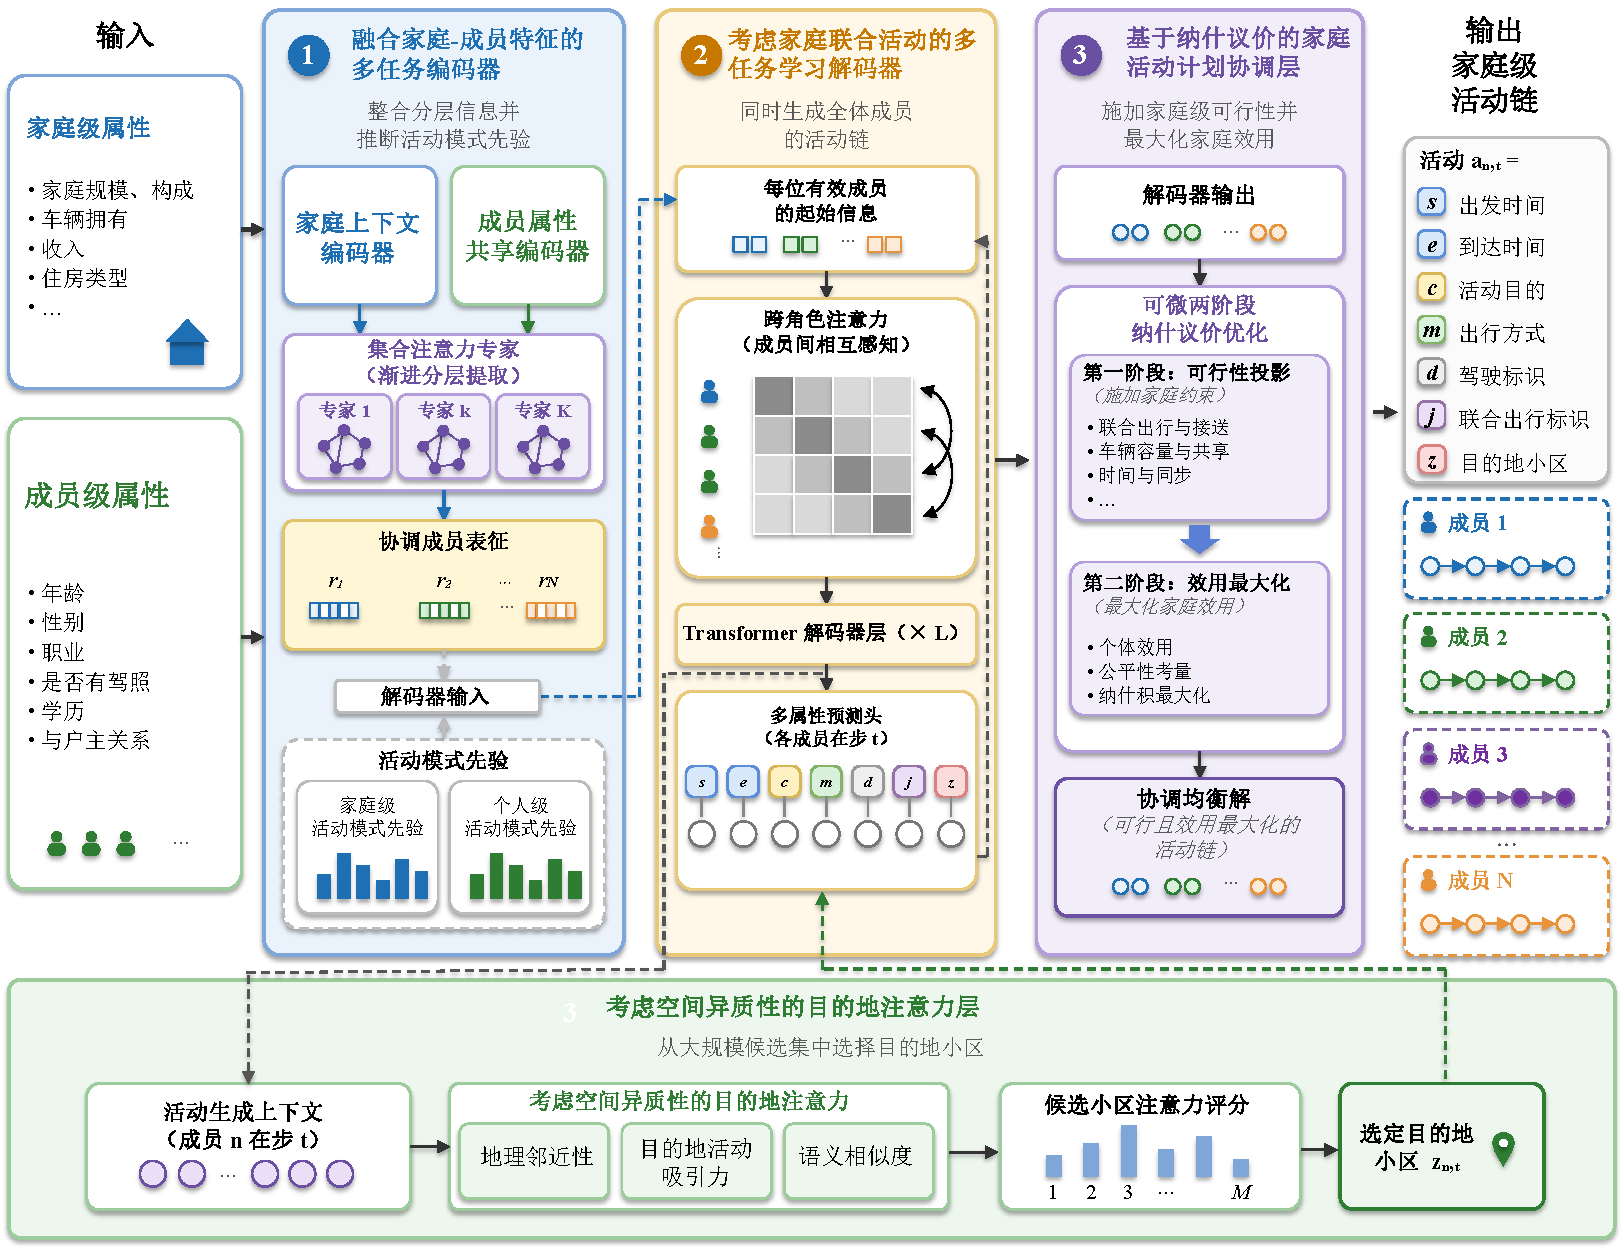
\includegraphics[width=\textwidth]{figures/ch4/model_framework_cn.pdf}
  \bicaption{考虑家庭联合活动的家庭级活动计划生成方法总体框架}{Overall framework of the household-level activity chain generation method with intra-household joint activities.}
  \label{fig.cohact.framework}
\end{figure}
 
%==================================================================
\section{融合家庭-成员特征的多任务编码器}\label{sec.cohact.encoder}

承接\ref{sec.cohact.intro}节的问题描述，本章将家庭级活动计划生成构建为一个条件生成任务：以家庭级属性向量 $\mathbf{h}\in\mathbb{R}^{d_h}$ 与各成员的属性向量 $\{\mathbf{P}_i\in\mathbb{R}^{d_p}\}_{i=1}^{N}$ 为条件，为家庭中每位有效成员生成完整的活动链，其中 $N$ 为家庭成员数。家庭级属性刻画家庭的共享特征，如家庭规模与构成、车辆拥有与收入水平；成员级属性刻画成员的个体特征，如年龄、性别、职业与持照状态；二者共同构成生成所依赖的条件信息。本节聚焦模型的输入侧，即如何将上述异质条件信息编码为指导后续家庭及活动计划生成的融合表征。编码器的整体结构如图~\ref{fig.cohact.encoder}所示。

\begin{figure}[H]
  \centering
  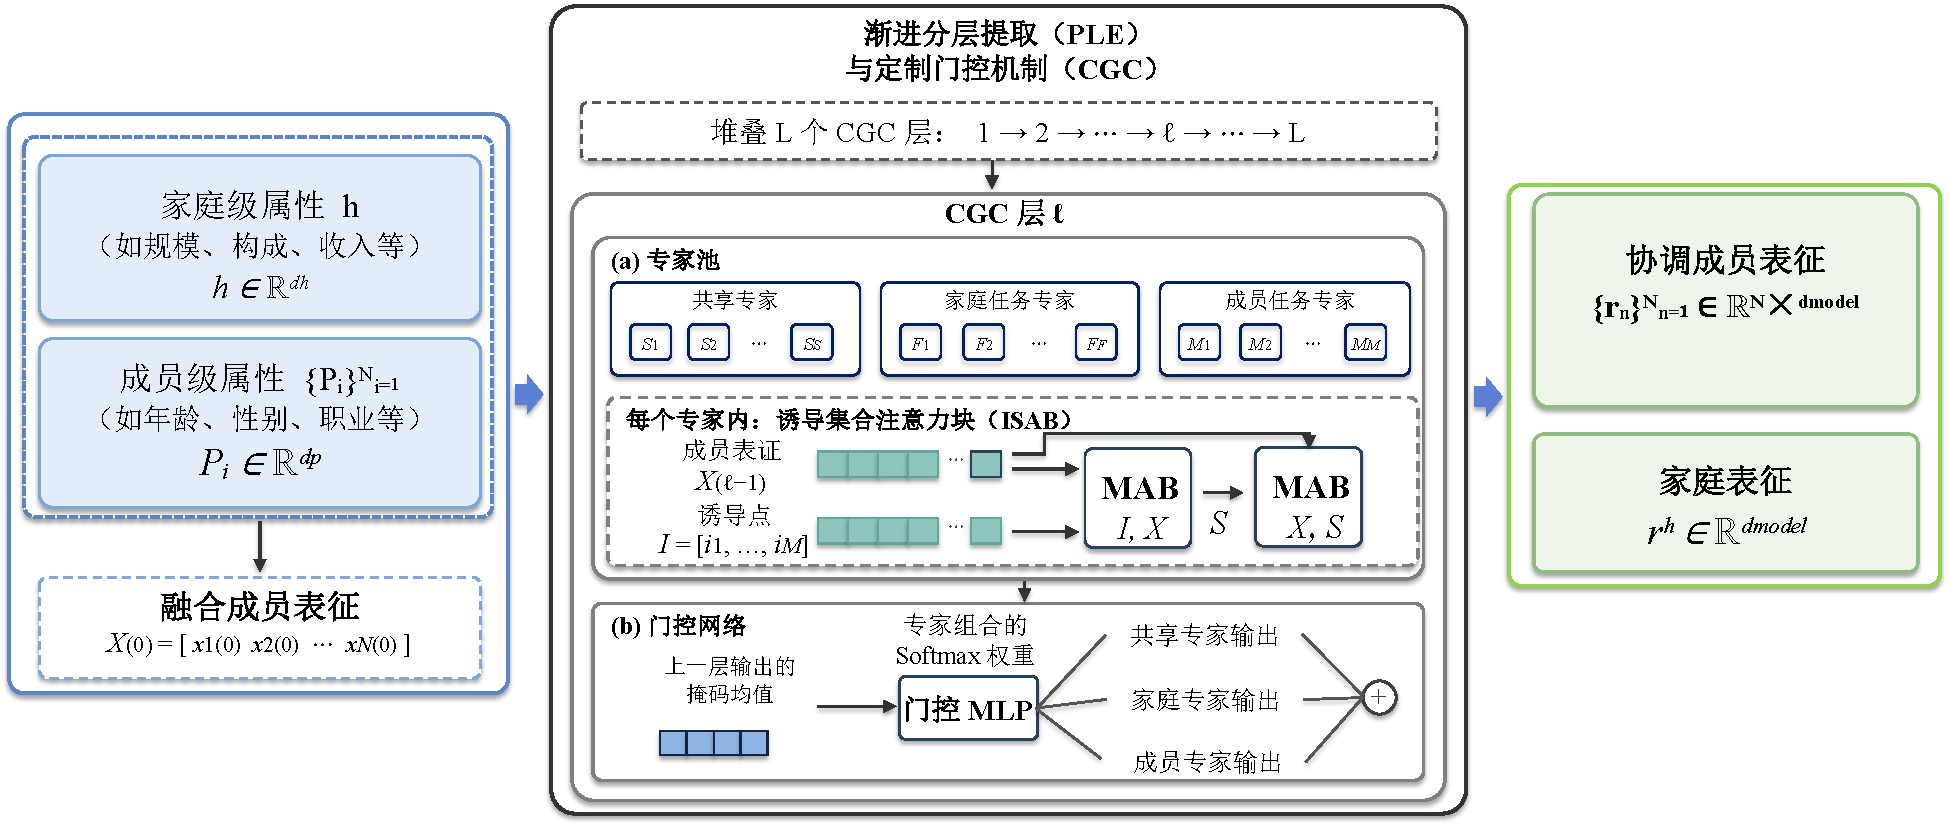
\includegraphics[width=\textwidth]{figures/ch4/encoder_framework_cn.pdf}
  \bicaption{融合家庭-成员特征的多任务编码器示意图}{Schematic diagram of the multi-task encoder integrating household and member features.}
  \label{fig.cohact.encoder}
\end{figure}

由\ref{sec.cohact.intro}所述，每位家庭成员的活动链同时受到家庭共享特征与成员个体属性的影响，二者粒度不同、视角互补，须在生成之前整合为统一的成员表征。为此，本节设计融合家庭-成员特征的多任务编码器，将家庭级与成员级属性映射为一组相互协调的成员表征以及一个家庭级表征，作为后续解码器的条件信息。编码器的设计出于两点考虑。一方面，家庭中的成员天然构成无序且规模可变的集合，编码器须对成员顺序保持置换等变、并能处理不同规模的家庭，同时应有效融合每位成员的特征与成员间共享的家庭级特征。另一方面，条件信息中家庭层面与成员层面的属性粒度不同：家庭规模、车辆拥有与收入水平等家庭属性对全体成员取值相同，刻画家庭的共享背景；年龄、职业与持照状态等成员属性则因人而异，刻画成员的个体差异。二者视角互补，编码器须在一定程度上将其解耦，方能在提取家庭共享特征的同时保留成员专属特征。基于上述两点考虑，本节首先设计融合家庭-成员特征的编码层，将家庭属性与成员属性融合为统一的成员表征；随后设计渐进分层提取（Progressive Layered Extraction, PLE）\citep{tangProgressiveLayeredExtraction2020}编码器，将家庭-成员特征融合问题建模为一个包含家庭表征与成员表征两项主任务的多任务学习问题，显式分离共享参数与任务专属参数，从而协调地学习家庭表征与成员表征；此外，为处理由属性到活动链的``一对多''问题，本节还构建家庭与个人级的活动模式先验，为后续生成提供模式层面的引导。设计的融合家庭-成员特征的多任务编码器的结构示意图如图~\ref{fig.cohact.encoder}所示。

\subsection{家庭-成员特征融合}

首先，构建家庭-成员特征融合层，将家庭级属性向量 $\mathbf{h}$ 与成员级属性矩阵 $\mathbf{P}=[\mathbf{P}_1,\dots,\mathbf{P}_N]^{\top}$ 整合为统一的成员表征。为使每位成员的信息向量有效融合成员共享的家庭属性与自身属性，首先将家庭属性向量广播至全体成员，并与各成员属性拼接，再经一个共享的线性层映射为维度为 $d_{\text{model}}$ 的融合表征：
\begin{equation}
\mathbf{x}_n^{(0)}=\mathrm{Linear}\!\left(\mathbf{h}\,\|\,\mathbf{P}_n\right)\in\mathbb{R}^{d_{\text{model}}},\quad n=1,\dots,N,
\label{eq.cohact.fuse}
\end{equation}
式中，$\|$ 表示向量拼接。将各成员的线性变换结果按行堆叠，即得融合表征矩阵 $\mathbf{X}^{(0)}=[\mathbf{x}_1^{(0)},\dots,\mathbf{x}_N^{(0)}]^{\top}\in\mathbb{R}^{N\times d_{\text{model}}}$，作为后续PLE编码器的输入。

\subsection{活动模式先验构建}

除式\refeq{eq.cohact.fuse}获取的融合表征外，编码器还须为后续生成提供活动模式先验，以缓解由属性到活动链的``一对多''映射，压缩解码器生成家庭级活动计划的生成空间。为此，本章在 $C_h$ 个家庭级与 $C_p$ 个个人级活动模式簇上分别构建家庭级活动模式分布 $\boldsymbol{\pi}^h\in\Delta^{C_h}$ 与各成员的个人级活动模式分布 $\{\boldsymbol{\pi}_n^{\text{ind}}\in\Delta^{C_p}\}_{n=1}^{N}$，其中 $\Delta^{C}$ 表示 $C$ 维概率单纯形。活动模式簇通过对训练集中的活动链施加高斯混合模型聚类离线获得，簇数由贝叶斯信息准则确定。活动模式分布并非由编码器主干预测，而是由一个独立训练、并经蒸馏得到的活动模式识别模型 $g_\phi$ 根据家庭与成员属性给出，且在 CoHACT 训练过程中冻结权重，以获取稳定的活动模式输出。以上模式条件生成与CoHACT相对分离的设计的优势在于：在训练早期编码器表征尚不稳定时，冻结的 $g_\phi$ 仍能提供稳定且具有信息量的模式先验，从而更可靠地引导生成。所得家庭与个人级活动模式分布将在\ref{sec.cohact.decoder}节经自适应层归一化注入解码过程。

\subsection{渐进分层提取编码器}

经式\refeq{eq.cohact.fuse}的特征融合，家庭属性与家庭成员属性被整合为融合表征矩阵 $\mathbf{X}^{(0)}$，其每一行对应一名成员，表示该成员的个体信息及其所属家庭的共享信息。在此基础上，编码器须进一步处理该表征矩阵以获取供解码器使用的两类特征：逐成员刻画的成员特征 $\mathbf{R}$，与刻画家庭整体的家庭特征 $\mathbf{r}^h$。须强调的是，家庭特征与成员特征与原始输入数据不同，应涵盖蕴含家庭层面的完整信息。具体而言，成员的活动计划制定受家庭情境制约——其他成员的属性、家庭共享的资源以及联合开展的活动均会影响单个成员的活动安排；家庭特征 $\mathbf{r}^h$ 则在此之上对全体成员作进一步汇聚，用以给解码器统筹家庭层面的整体安排。

正因两类特征高度共享信息而又各有侧重，若以单一共享网络学习，家庭特征与成员特征提取两项任务在训练过程中的梯度易相互干扰，引发模型输出效果在两类特征间此消彼长的``跷跷板''效应（多任务学习中经典的负迁移问题）。为此，本节将编码过程建模为一个包含成员特征提取与家庭特征提取两项主任务的多任务学习问题，并采用渐进分层提取（Progressive Layered Extraction, PLE）\citep{tangProgressiveLayeredExtraction2020}结构作为编码器主体，显式分离两项任务的共享参数与专属参数，从而在充分共享公共信息的同时协调地提取两类特征。

PLE结构堆叠 $L$ 个定制门控（Customized Gate Control, CGC）层。每个 CGC 层为两项特征提取任务设置 $m_s$ 个对全体任务可见的共享专家，并为每项任务各配置 $m_k$ 个任务专属专家：共享专家提取家庭与成员中的融合信息，任务专属专家保留各自任务的特性，使每项任务既能利用共享专家提取的融合信息、又能借助专属专家维持自身特性，从而缓解任务间的负迁移现象。

每个专家的输入为按成员排布的特征矩阵，首层取融合表征矩阵 $\mathbf{X}^{(0)}$。由于家庭内成员本无固定次序、且家庭规模随家庭而异，专家须对成员的排列保持置换等变，并适应可变的成员数目。为此，本章将每个专家建模为诱导集合注意力块（Induced Set-Attention Block, ISAB）\citep{leeSetTransformerFramework2019}，使各成员的提取后的特征均由全体成员的特征聚合而来，既不依赖成员次序与家庭规模，又使各成员的提取后特征蕴含家庭层面的信息。ISAB 的基本组件为多头注意力块（Multi-head Attention Block, MAB）。给定查询矩阵 $\mathbf{Q}$ 与键矩阵 $\mathbf{K}$，MAB 定义为
\begin{equation}
\mathrm{MAB}(\mathbf{Q},\mathbf{K})=\mathrm{LN}\!\left(\mathbf{A}+\mathrm{FFN}(\mathbf{A})\right),\quad \mathbf{A}=\mathrm{LN}\!\left(\mathbf{Q}+\mathrm{MHA}(\mathbf{Q},\mathbf{K},\mathbf{K})\right),
\label{eq.cohact.mab}
\end{equation}
式中，$\mathrm{MHA}(\cdot)$ 为多头注意力，$\mathrm{FFN}(\cdot)$ 为逐位置前馈网络，$\mathrm{LN}(\cdot)$ 为层归一化。直接对 $N$ 个成员的特征施加自注意力的复杂度为 $O(N^{2}d_{\text{model}})$，且不显式产生家庭层面的聚合特征，不利于每个成员获取家庭层面的信息。为此，ISAB 引入一组数量为 $n_I$ 的可学习诱导点 $\mathbf{I}\in\mathbb{R}^{n_I\times d_{\text{model}}}$，经两个堆叠的 MAB 计算各成员的提取后特征：
\begin{equation}
\mathbf{S}=\mathrm{MAB}(\mathbf{I},\mathbf{X})\in\mathbb{R}^{n_I\times d_{\text{model}}},\qquad \mathrm{ISAB}(\mathbf{X})=\mathrm{MAB}(\mathbf{X},\mathbf{S})\in\mathbb{R}^{N\times d_{\text{model}}},
\label{eq.cohact.isab}
\end{equation}
即诱导点先对成员集合施加注意力，形成紧凑的家庭级聚合特征 $\mathbf{S}$；各成员再以自身为查询对象、对该家庭级聚合特征施加注意力，得到各自的提取后特征。如此，计算复杂度由 $O(N^{2}d_{\text{model}})$ 降至 $O(N n_I\,d_{\text{model}})$，且各成员的提取后特征均经由对家庭级聚合特征的注意力计算得到，故蕴含家庭层面的信息。

基于 ISAB 专家，CGC 层以门控机制耦合两项特征提取任务，使每项任务按各自的组合权重读取其专属专家与全部共享专家的提取后特征。对第 $\ell$ 层的任务 $k$，记其自上一层得到的提取后特征矩阵为 $\mathbf{U}_k^{(\ell-1)}\in\mathbb{R}^{N\times d_{\text{model}}}$，并以 $\mathbf{U}_k^{(0)}=\mathbf{X}^{(0)}$ 初始化。门控网络依据掩码均值 $\bar{\mathbf{u}}_k^{(\ell-1)}$ 计算任务 $k$ 在其候选专家集上的组合权重，其中有效成员掩码 $\mu_n^{\text{mem}}$ 用于屏蔽为对齐最大家庭规模而填充的无效成员位：
\begin{equation}
\mathbf{w}_k^{(\ell)}=\mathrm{Softmax}\!\left(\mathbf{W}_k^{(\ell)}\,\bar{\mathbf{u}}_k^{(\ell-1)}\right),\qquad \bar{\mathbf{u}}_k^{(\ell-1)}=\frac{\sum_{n=1}^{N}\mu_n^{\text{mem}}\,\mathbf{u}_{k,n}^{(\ell-1)}}{\sum_{n=1}^{N}\mu_n^{\text{mem}}},
\label{eq.cohact.gate}
\end{equation}
式中，$\mathbf{u}_{k,n}^{(\ell-1)}$ 为矩阵 $\mathbf{U}_k^{(\ell-1)}$ 的第 $n$ 行，即成员 $n$ 的提取后特征向量，$\mathrm{Softmax}(\cdot)$ 沿候选专家维度归一化，$\mathbf{W}_k^{(\ell)}$ 为任务 $k$ 在第 $\ell$ 层的可学习门控矩阵。任务 $k$ 在第 $\ell$ 层的提取后特征为其全部候选专家输出的加权组合：
\begin{equation}
\mathbf{U}_k^{(\ell)}=\sum_{e=1}^{m_s+m_k} w_{k,e}^{(\ell)}\,\mathrm{E}_{k,e}^{(\ell)}\!\left(\mathbf{U}_k^{(\ell-1)}\right),
\label{eq.cohact.cgc}
\end{equation}
式中，$\mathrm{E}_{k,e}^{(\ell)}(\cdot)$ 为任务 $k$ 可用的第 $e$ 个专家的特征提取函数，即式\refeq{eq.cohact.isab}的 ISAB 计算流程，专家候选集涵盖 $m_s$ 个共享专家与 $m_k$ 个任务专属专家，$w_{k,e}^{(\ell)}$ 为式\refeq{eq.cohact.gate}所得的相应门控权重。如此，两项主任务依据各自门控权重对共享专家与专属专家作加权计算，并随 CGC 层的堆叠逐层细化各自的提取后特征。

经 $L$ 个 CGC 层后，成员特征提取任务以其末层提取后特征作为成员特征矩阵 $\mathbf{R}=[\mathbf{r}_1,\dots,\mathbf{r}_N]^{\top}\in\mathbb{R}^{N\times d_{\text{model}}}$，家庭特征提取任务则对其末层提取后特征在各有效成员位置上施加掩码均值池化，得到家庭表征 $\mathbf{r}^h\in\mathbb{R}^{d_{\text{model}}}$。所得成员表征与家庭表征连同前文构建的活动模式先验一并传输给解码器，用于生成家庭中各成员的活动链。
 
\section{考虑家庭联合活动的多任务学习解码器}\label{sec.cohact.decoder}

承接\ref{sec.cohact.encoder}节的编码器，本节设计考虑家庭联合活动的活动计划解码器，以编码器输出的成员表征 $\{\mathbf{r}_n\}_{n=1}^{N}$、家庭表征 $\mathbf{r}^h$ 与家庭、个人级活动模式先验为条件，为家庭中每位有效成员生成完整的活动计划。记成员 $n$ 的活动计划为按时序排列的活动序列 $\{a_{n,t}\}_{t=1}^{T}$，$T$ 为最大链长；每个活动 $a_{n,t}$ 由刻画其时间、空间与行为特征的七个属性构成：
\begin{equation}
a_{n,t}=\left(s_{n,t},\ e_{n,t},\ c_{n,t},\ m_{n,t},\ d_{n,t},\ j_{n,t},\ z_{n,t}\right),
\label{eq.cohact.tuple}
\end{equation}
式中，$s_{n,t},e_{n,t}\in\mathbb{R}$ 为归一化的出发与到达时间；$c_{n,t}$ 为活动目的；$m_{n,t}$ 为出行方式；$d_{n,t}$ 与 $j_{n,t}$ 为驾驶与联合出行的二元标识；$z_{n,t}$ 为目的地小区。值得注意的是，生成的目标是家庭而非个体，即同时生成全体成员的活动计划，并显式建模与满足家庭的联合出行需求。

现实中，居民的活动决策同时受自身属性与家庭情境的约束，且须确定活动的多个属性——参与何种活动、于何时何地开展、以及如何在活动间出行。因此，家庭级活动计划生成既须同时考虑全体成员、又须兼顾活动的全部属性，可自然地建模为一个多任务序列生成问题。为此，本节将解码器设计为以每个活动属性为一项任务的多任务注意力网络，即由一个任务特定注意力与一组专属预测头共同构成 MTAN 式解码器\citep{liuEndtoEndMultiTaskLearning2019}。生成过程分两个阶段组织：第一阶段，由成员表征与家庭表征构建家庭级特征，并经跨角色注意力使成员间相互交互，获得家庭成员的协调特征，表示家庭成员在认知家庭情境与其他成员的基础上形成的协调表征；第二阶段，以该成员特征、成员表征与活动模式先验为条件，由共享的 Transformer 解码器自回归地生成各成员的活动序列，再由专属预测头给出各活动属性。

上述设计针对\ref{sec.cohact.intro}节的难点\cp{2}与\cp{3}。其中，难点\cp{2}的协调生成由解码器经跨角色注意力使各成员相互感知、并同时生成全体成员的活动计划解决，而车辆可用性等不可违反的硬约束则由后续基于纳什议价的家庭活动计划协调层控制；难点\cp{3}的目的地选择由考虑空间异质性的目的地与出行方式联合预测方法处理，在城市尺度的大候选集上联合预测目的地与出行方式。

据此，本节分两部分展开：首先，构建家庭成员特征协调层以获取相互作用的家庭成员特征（\ref{subsec.cohact.coord}小节）；随后，设计自回归活动计划生成器（\ref{subsec.cohact.autoreg}小节。家庭协调式活动链解码器的总体结构如图~\ref{fig.cohact.decoder}所示。

\begin{figure}[H]
  \centering
  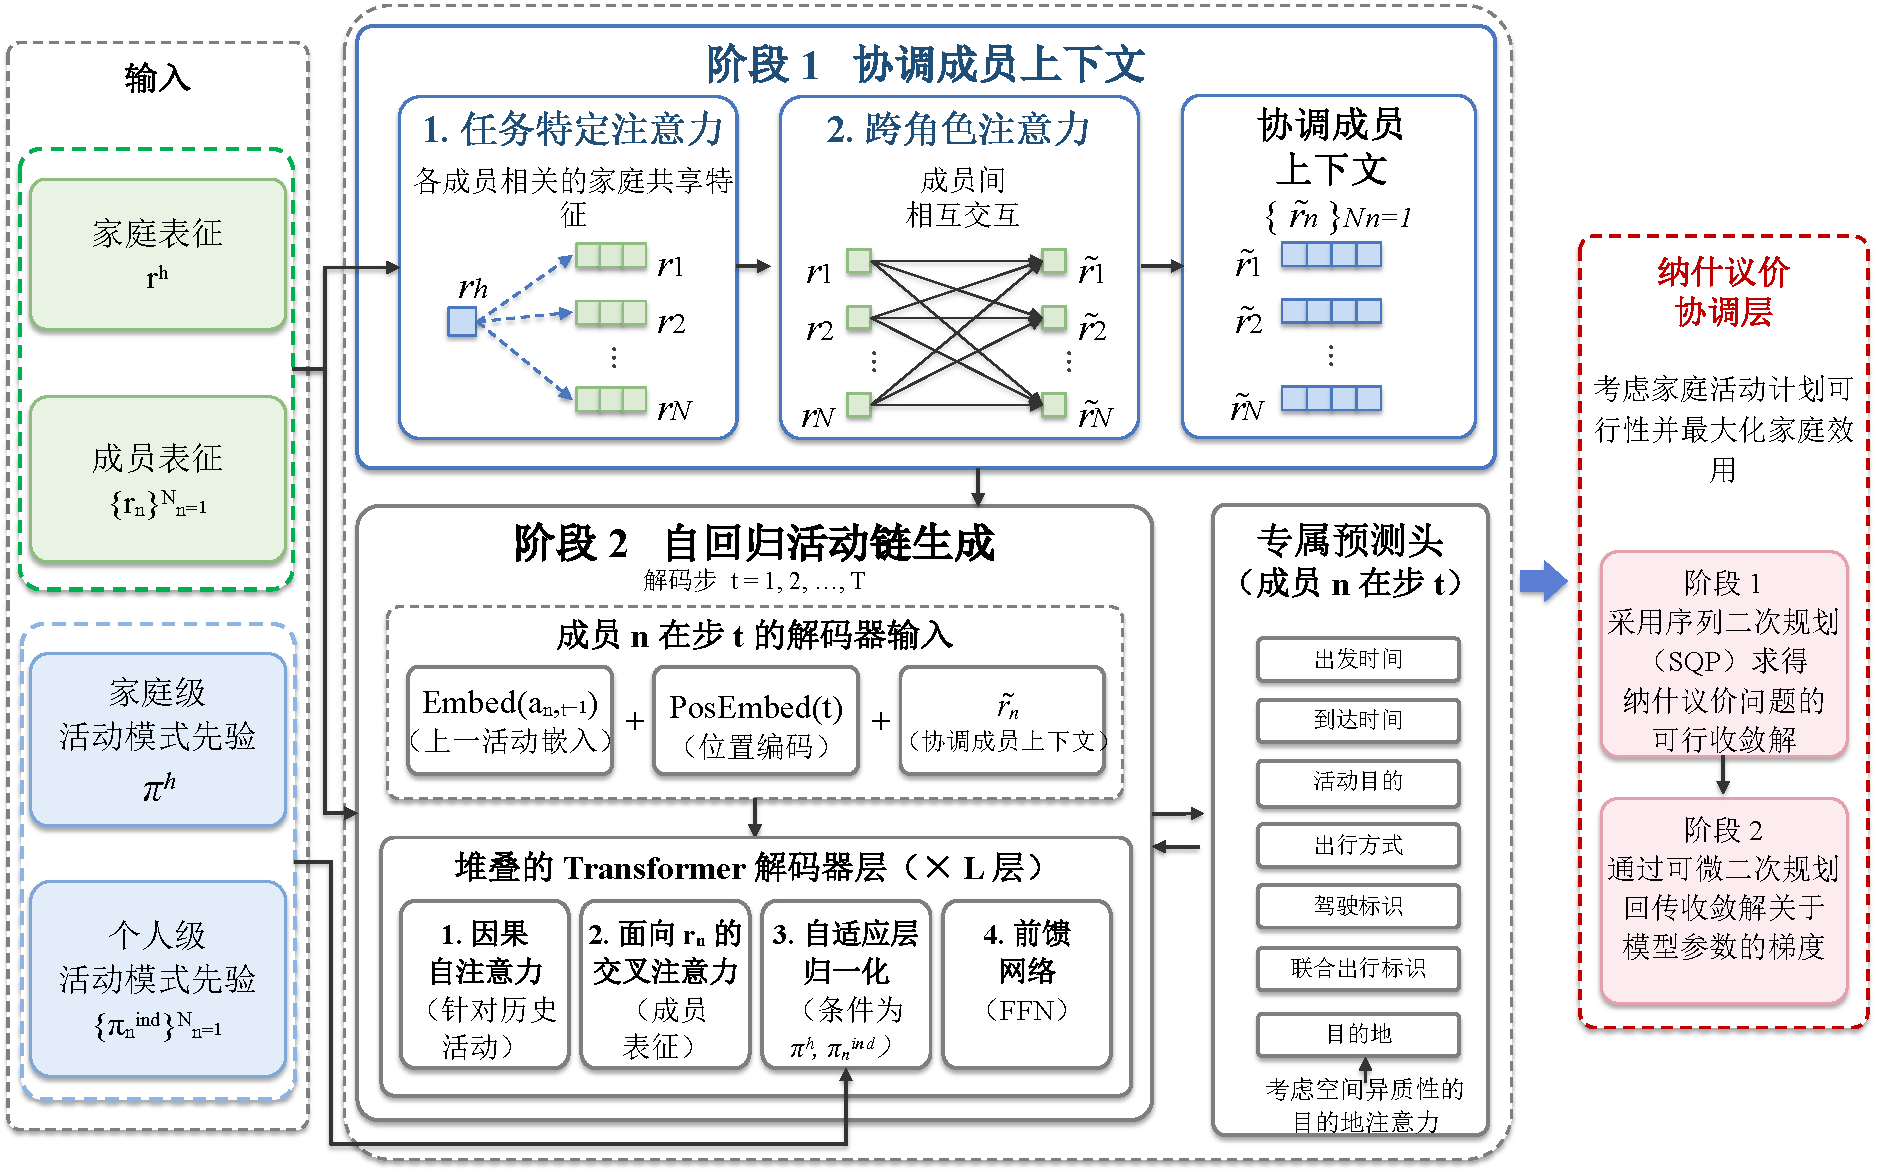
\includegraphics[width=\textwidth]{figures/ch4/decoder_framework_cn.pdf}
  \bicaption{家庭协调式活动链解码器示意图}{Schematic diagram of the household-coordinated activity-chain decoder.}
  \label{fig.cohact.decoder}
\end{figure}

\subsection{家庭成员特征协调层}\label{subsec.cohact.coord}

经编码器得到的成员特征 $\mathbf{R}=[\mathbf{r}_1,\dots,\mathbf{r}_N]^{\top}$ 已由编码器中的共享专家与任务专属专家输出的特征聚合得到，每位成员的特征均隐含家庭整体与其余成员的信息；家庭特征 $\mathbf{r}^h$ 则是面向家庭特征任务的整体概括。为使各成员在自回归生成活动计划时据考虑到车辆共享与接送时序等联合活动，本节在自回归生成前设置特征协调层，依次使用任务特定注意力与跨角色注意力对成员特征作两步增强：前者将家庭特征 $\mathbf{r}^h$ 显式注入各成员特征，后者在成员间显式交互，二者共同输出供解码器使用的协调成员特征 $\{\tilde{\mathbf{r}}_n\}$，表示家庭成员在认知家庭情境与其他成员的基础上形成的协调表征。

首先，任务特定注意力使每位成员从编码器输出的家庭特征中提取与自身相关的家庭共享特征。该注意力以成员特征 $\mathbf{r}_n$ 为查询向量、以家庭表征 $\mathbf{r}^h$ 为键向量与值向量，二者分别取自编码器的成员表征任务与家庭表征任务，故称任务特定：
\begin{equation}
\bar{\mathbf{r}}_n=\mathrm{LN}\!\left(\mathbf{r}_n+\mathrm{MHA}\!\left(\mathbf{r}_n,\,\mathbf{r}^h,\,\mathbf{r}^h\right)\right),
\label{eq.cohact.famattn}
\end{equation}
式中，$\mathrm{MHA}(\cdot)$ 为多头注意力；$\mathrm{LN}(\cdot)$ 为层归一化；$\bar{\mathbf{r}}_n$ 为提取家庭共享特征后的成员表征。

随后，跨角色注意力在有效成员集合上采用多头自注意力，使各成员相互交互，以捕捉家庭内部的活动计划协调关系：
\begin{equation}
\tilde{\mathbf{r}}_n=\mathrm{LN}\!\left(\bar{\mathbf{r}}_n+\mathrm{MHA}\!\left(\bar{\mathbf{r}}_n,\,\bar{\mathbf{R}},\,\bar{\mathbf{R}}\right)\right),
\label{eq.cohact.roleattn}
\end{equation}
式中，$\bar{\mathbf{R}}=[\bar{\mathbf{r}}_1,\dots,\bar{\mathbf{r}}_N]^{\top}$ 为全体成员提取家庭共享特征后的成员表征，注意力由有效成员掩码 $\mu_n^{\text{mem}}$ 屏蔽，使填充的无效成员不参与计算；$\tilde{\mathbf{r}}_n$ 为最终得到的每个成员的协调成员特征。

经上述两步，协调成员特征 $\{\tilde{\mathbf{r}}_n\}_{n=1}^{N}$ 中的每位成员同时感知家庭信息与其余成员的信息，蕴含家庭层面的整体情境与成员间的协调关系，是后续自回归生成活动计划的输入。

\subsection{自回归活动计划生成器}\label{subsec.cohact.autoreg}

活动计划中的各活动相互关联，后一活动以先前已生成的活动为条件，天然契合自回归生成范式。为此，解码器以 $L_d$ 层堆叠的Transformer解码器逐步生成每位成员的活动序列。在步 $t$，对每个位置 $\tau\le t$，输入由上一次活动的嵌入、位置编码与协调成员特征，获取每位成员的活动表征 $\mathbf{u}_n^{(\tau)}$：
\begin{equation}
\mathbf{u}_n^{(\tau)}=\mathrm{Embed}\!\left(a_{n,\tau-1}\right)+\mathrm{PosEmbed}(\tau)+\tilde{\mathbf{r}}_n,
\label{eq.cohact.decin}
\end{equation}
式中，$\mathrm{Embed}(\cdot)$ 将上一次活动的属性嵌入，其中类别属性经嵌入表映射、连续属性经线性投影；$\mathrm{PosEmbed}(\tau)$ 为位置编码；$a_{n,0}$ 为可学习的起始向量；$\tilde{\mathbf{r}}_n$ 为成员 $n$ 的协调成员特征。

记输入序列 $\mathbf{H}^{(0)}=[\mathbf{u}_n^{(1)},\dots,\mathbf{u}_n^{(t)}]$（为简洁略去成员下标），第 $\ell$ 层Transformer解码器依次执行四个模块：

\textbf{其一，因果自注意力沿活动序列捕捉时序依赖}，并以下三角因果掩码 $\mathbf{M}$ 使每个位置的活动生成仅注意其之前的活动，保持自回归性：
\begin{equation}
\mathbf{H}'=\mathrm{LN}\!\left(\mathbf{H}^{(\ell-1)}+\mathrm{MHA}\!\left(\mathbf{H}^{(\ell-1)},\mathbf{H}^{(\ell-1)},\mathbf{H}^{(\ell-1)};\,\mathbf{M}\right)\right),
\label{eq.cohact.decself}
\end{equation}
式中，$\mathbf{M}$ 为下三角因果掩码，阻止该位置的活动生成受到未来活动的影响，$\mathbf{H}'$ 为因果自注意力后的活动表征。

\textbf{其二，面向成员特征的交叉注意力}以活动表征$\mathbf{H}'$为查询向量、以编码器输出的成员特征 $\mathbf{r}_n$ 为键向量与值向量，使生成在每一步均锚定于该成员的静态画像、避免长序列上发生漂移；家庭特征与其余成员的信息已由式\refeq{eq.cohact.decin}中的协调成员特征 $\tilde{\mathbf{r}}_n$ 注入输入：
\begin{equation}
\mathbf{H}''=\mathrm{LN}\!\left(\mathbf{H}'+\mathrm{MHA}\!\left(\mathbf{H}',\mathbf{r}_n,\mathbf{r}_n\right)\right).
\label{eq.cohact.deccross}
\end{equation}
式中，$\mathbf{H}''$ 为交叉注意力后的活动表征。

\textbf{其三，自适应层归一化}以家庭级与个人级活动模式分布为条件，对生成过程进行调制。两分布分别经投影、拼接后作为条件向量，再由一个轻量网络据此预测缩放与平移参数，用于调制层归一化：
\begin{equation}
(\boldsymbol{\gamma}_n,\boldsymbol{\beta}_n)=\mathrm{MLP}_{\text{ada}}\!\left(\mathrm{SiLU}\!\left(\left[\mathbf{W}^{h}\boldsymbol{\pi}^{h}\,\|\,\mathbf{W}^{\text{ind}}\boldsymbol{\pi}_n^{\text{ind}}\right]\right)\right),
\label{eq.cohact.adaln1}
\end{equation}
\begin{equation}
\mathbf{H}'''=(1+\boldsymbol{\gamma}_n)\odot\mathrm{LN}(\mathbf{H}'')+\boldsymbol{\beta}_n,
\label{eq.cohact.adaln2}
\end{equation}
式中，$\mathbf{W}^{h}$ 与 $\mathbf{W}^{\text{ind}}$ 将家庭级与个人级活动模式分布 $\boldsymbol{\pi}^{h},\boldsymbol{\pi}_n^{\text{ind}}$ 投影至隐藏层维度；$\odot$ 为逐元素相乘；$\mathrm{MLP}_{\text{ada}}$ 的末层参数初始化为零，使训练初期 $\boldsymbol{\gamma}_n$ 与 $\boldsymbol{\beta}_n$ 均为零、调制退化为恒等映射（此时 $\mathbf{H}'''=\mathrm{LN}(\mathbf{H}'')$），其后随训练逐步学到有效的调制，从而稳定训练。借助这一条件调制，同一套解码器即可依据活动模式条件适配不同类型的家庭（如通勤主导与接送主导的家庭），而无需为每类家庭单独设置子网络。最终，$\mathbf{H}'''$ 为自适应层归一化后的活动表征。

\textbf{其四，逐位置前馈网络}精炼各活动表征：
\begin{equation}
\mathbf{H}^{(\ell)}=\mathrm{LN}\!\left(\mathbf{H}'''+\mathrm{FFN}(\mathbf{H}''')\right).
\label{eq.cohact.decffn}
\end{equation}
式中，$\mathbf{H}^{(\ell)}$ 为第 $\ell$ 层的活动表征。

经 $L_d$ 层后，末位置的隐状态 $\mathbf{g}_n^{(t)}=\mathbf{H}^{(L_d)}[t]$ 送入一组专属预测头，预测得到步 $t$ 活动的各属性：
\begin{equation}
\begin{aligned}
(\hat{s}_{n,t},\,\hat{e}_{n,t}) &= \mathrm{MLP}_{\text{time}}\!\left(\mathbf{g}_n^{(t)}\right), \\
\hat{\mathbf{c}}_{n,t} &= \mathrm{Softmax}\!\left(\mathbf{W}_c\mathbf{g}_n^{(t)}\right), \\
\hat{\mathbf{d}}_{n,t} &= \mathrm{Softmax}\!\left(\mathbf{W}_d\mathbf{g}_n^{(t)}\right), \\
\hat{\mathbf{j}}_{n,t} &= \mathrm{Softmax}\!\left(\mathbf{W}_j\mathbf{g}_n^{(t)}\right).
\end{aligned}
\label{eq.cohact.heads}
\end{equation}
式中，$\mathrm{MLP}_{\text{time}}(\cdot)$ 为预测出发与到达时间 $(\hat{s}_{n,t},\hat{e}_{n,t})$ 的连续时间头；$\mathbf{W}_c$、$\mathbf{W}_d$、$\mathbf{W}_j$ 分别为活动目的、驾驶与联合出行分类头的投影矩阵，$\hat{\mathbf{c}}_{n,t}$ 为活动目的的类别分布，$\hat{\mathbf{d}}_{n,t}$、$\hat{\mathbf{j}}_{n,t}$ 为驾驶与联合出行二元标识的分布。目的地 $z_{n,t}$ 与出行方式 $m_{n,t}$预测，均以解码隐状态 $\mathbf{g}_n^{(t)}$ 为输入，二者在空间维度上高度相关，即活动目的地的选择直接影响出行方式的选择，反之亦然。

为此，将目的地与出行方式的预测耦合建模，进一步设计考虑空间异质性的目的地与出行方式联合预测方法，以在城市尺度的大候选集上联合预测目的地与出行方式。

首先，为异质地表征候选目的地，每个候选目的地 $z\in\mathcal{Z}$ 由三组特征刻画：可学习的目的地嵌入 $\mathbf{e}_z$，以数据驱动方式捕捉每个目的地的潜在特性；预计算的 LDA 主题向量 $\boldsymbol{\ell}_z$，由目的地内兴趣点（Point Of Interest，POI）分布概括其用地构成；预计算的吸引力向量 $\mathbf{a}_z\in\mathbb{R}^{P}$，其各分量为各候选目的地内与各活动目的相关的设施数量。三组特征拼接后投影至隐藏层维度，得到各候选目的地的键向量：
\begin{equation}
\mathbf{k}_z=\mathbf{W}_k\,\mathrm{LN}\!\left(\mathrm{MLP}\!\left(\left[\mathbf{e}_z\,\|\,\boldsymbol{\ell}_z\,\|\,\mathbf{a}_z\right]\right)\right)\in\mathbb{R}^{d_{\text{model}}},
\label{eq.cohact.zonekey}
\end{equation}
式中，$\mathrm{MLP}(\cdot)$ 为带层归一化的两层网络；$\mathbf{W}_k$ 为键投影矩阵；$\|$ 表示拼接；$P$ 为活动目的数。全部候选目的地键 $\mathbf{K}=[\mathbf{k}_1,\dots,\mathbf{k}_{|\mathcal{Z}|}]^{\top}$ 每次前向只计算一次，并在全体成员与活动步间共享。

随后，以当前活动的生成隐状态$\mathbf{g}_n^{(t)}$与目的意图为查询向量，对候选目的地评分。对成员 $n$ 的第 $t$ 次活动，查询由解码隐状态、出发地嵌入与所预测的活动目的融合而成：
\begin{equation}
\mathbf{q}_{n,t}=\mathrm{MLP}_q\!\left(\left[\mathbf{g}_n^{(t)}\,\|\,\mathbf{o}_{n,t}\,\|\,\hat{\mathbf{c}}_{n,t}\right]\right)\in\mathbb{R}^{d_{\text{model}}},
\label{eq.cohact.destquery}
\end{equation}
式中，$\mathbf{o}_{n,t}$ 为出发地小区的嵌入，即上一活动的目的地（首个活动则为当前位置）；$\hat{\mathbf{c}}_{n,t}$ 为所预测的活动目的分布。继而对每个候选目的地评分，并以地理阻抗惩罚与目的吸引力加成增强注意力：
\begin{equation}
\mathrm{logit}_{n,t,z}=\frac{\mathbf{q}_{n,t}^{\top}\mathbf{k}_z}{\sqrt{d_{\text{model}}}}-\lambda_{\text{imp}}\,\delta_{o_{n,t},z}+\lambda_{\text{aff}}\,\mathbf{a}_z^{\top}\hat{\mathbf{c}}_{n,t},
\label{eq.cohact.destlogit}
\end{equation}
式中，$\frac{\mathbf{q}_{n,t}^{\top}\mathbf{k}_z}{\sqrt{d_{\text{model}}}}$为查询向量与候选目的地键向量的相似度；$\delta_{o_{n,t},z}$ 为由出发地 $o_{n,t}$ 至候选目的地 $z$ 的预计算阻抗，惩罚项 $-\lambda_{\text{imp}}\delta_{o_{n,t},z}$ 实现类似引力模型的距离衰减；$\mathbf{a}_z^{\top}\hat{\mathbf{c}}_{n,t}$ 为候选目的地 $z$ 在所预测目的下的期望的吸引力，奖励对该目的更具吸引力的小区；权衡系数 $\lambda_{\text{imp}},\lambda_{\text{aff}}>0$ 均可学习。最终对全候选目的地上的评分 $\mathrm{logit}_{n,t,z}$进行 Softmax 运算得到目的地预测的概率分布：
\begin{equation}
P\!\left(z_{n,t}=z\right)=\frac{\exp\!\left(\mathrm{logit}_{n,t,z}\right)}{\sum_{z'\in\mathcal{Z}}\exp\!\left(\mathrm{logit}_{n,t,z'}\right)}.
\label{eq.cohact.destsoftmax}
\end{equation}

考虑到出行方式与出行距离密切相关，而出行距离取决于所选目的地。为此，以距离感知的出行方式预测头显式耦合方式预测与目的地选择。先由目的地分布与阻抗矩阵计算活动的期望出行距离：
\begin{equation}
\bar{\delta}_{n,t}=\sum_{z\in\mathcal{Z}}P\!\left(z_{n,t}=z\right)\,\delta_{o_{n,t},z},
\label{eq.cohact.expdist}
\end{equation}
随后，以解码隐状态 $\mathbf{g}_n^{(t)}$ 与期望距离为输入给出对出行方式的基础预测，再叠加距离-方式先验偏置 $\mathbf{b}(\bar{\delta}_{n,t})$，得到出行方式分布：
\begin{equation}
\hat{\mathbf{m}}_{n,t}=\mathrm{Softmax}\!\left(\mathrm{MLP}_m\!\left(\left[\mathbf{g}_n^{(t)}\,\|\,\bar{\delta}_{n,t}\right]\right)+\mathbf{b}\!\left(\bar{\delta}_{n,t}\right)\right).
\label{eq.cohact.mode}
\end{equation}
式中，$\bar{\delta}_{n,t}$ 为按目的地分布加权的期望出行距离；$\mathrm{MLP}_m(\cdot)$ 为出行方式分类头；$\mathbf{b}(\bar{\delta}_{n,t})$ 为由训练集距离-方式经验分布初始化的先验偏置。
 
%==================================================================
%==================================================================
\section{基于纳什议价的家庭活动计划协调层}\label{sec.cohact.nash}
% 对应英文稿 §3.4；解决难点\cp{2}·可行性

\ref{sec.cohact.decoder}节的解码器虽借助跨角色注意力等机制使各成员生成的活动计划相互呼应，但其输出仍为概率分布与连续值等“软”形式，并未在成员之间显式施加家庭层面的硬约束，易导致生成的活动计划在家庭层面不可行，对应生成任务中的“结构零”问题。实际上，家庭的一日活动计划本质上是家庭成员共享有限资源、并在部分冲突的活动计划间相互妥协的集体决策：一方面，成员日程受不可违反的硬约束限制，如同时驾车的成员数不能超过家庭车辆数、联合出行的成员须共享一致的出发到达时间与出行方式；另一方面，满足这些耦合还需在成员间权衡，如谁占用有限车辆、谁接送孩子等受抚养成员、谁的活动时间被调整，故协调后的日程是协商折中而非任一成员的最优。因此，解码器的输出至多在统计上促成协调，却既不能严格保证上述家庭层面硬性约束成立，也难以化解成员间的资源冲突（难点\cp{2}的可行性）。

为此，在解码器生成家庭级别的活动计划后，本节将家庭活动计划协调任务建模为一个纳什议价（Nash Bargaining）问题，提出基于纳什议价的家庭活动计划协调层，将解码器输出的活动计划投影到家庭层面可行的均衡解。具体而言，以解码器输出的各家庭成员的活动计划为参考活动计划，求解一个帕累托有效、个体理性（任一成员协商后的效用不劣于其单独行动获得的效用）且在成员间均衡分配效用增益的可行解，使家庭活动计划协调结果在严格满足家庭资源约束与联合活动约束的同时，能够最大程度地提升家庭整体效用。为保证提出的纳什议价协调层可与编码器与解码器端到端联合训练，本节进一步设计两阶段的可微优化算法，即先求解纳什议价问题以获得协调解、再经优化过程反向传播梯度，从而既施加家庭级可行性、又将协调信号回传以引导编码器与解码器的学习。

\subsection{问题构建}\label{subsec.cohact.nash.problem}

\textbf{（1）纳什议价模型}

纳什议价模型源于合作博弈论\citep{nashBargainingProblem1950}，刻画多个参与者就一组可行结果进行协商、并在无法达成一致时各自退守至某一分歧点（disagreement point）的情形。设有 $N$ 个参与者，其可达成的效用向量构成可行集 $\mathcal{S}\subseteq\mathbb{R}^{N}$，分歧点 $\mathbf{u}^{0}=(u_1^{0},\dots,u_N^{0})$ 为协商破裂时各参与者所得的效用。纳什证明，在帕累托有效、对称、仿射变换不变与无关方案独立四条公理下，存在唯一的议价解，其最大化各参与者相对分歧点的效用增益之积：
\begin{equation}
\mathbf{u}^{\star}=\arg\max_{\mathbf{u}\in\mathcal{S},\,\mathbf{u}\ge\mathbf{u}^{0}}\;\prod_{n=1}^{N}\bigl(u_n-u_n^{0}\bigr).
\label{eq.cohact.nashclassic}
\end{equation}
式中，$\mathbf{u}^{\star}$ 为纳什议价解，兼具个体理性（任一参与者协商后的效用不劣于其单独行动获得的效用））与帕累托有效性，并在参与者间均衡分配增益、而非简单最大化效用之和，因而广泛用于刻画资源分配与利益协调问题。

\textbf{（2）家庭活动计划协调问题建模}

本节将家庭活动计划的协调建模为一个纳什议价问题：家庭成员即参与者，各成员未经协调的解码器生成的活动计划构成其分歧点，可行集为满足家庭资源约束与联合活动约束的协调活动计划。具体而言，设有 $N$ 个家庭成员，其可达成的效用向量构成可行集 $\mathcal{F}\subseteq\mathbb{R}^{N}$，分歧点 $\mathbf{U}^{0}=(U_1^{0},\dots,U_N^{0})$ 为各成员从解码器生成的活动计划中获得的效用。基于纳什议价的家庭活动计划协调模型的目标是求解一个帕累托有效、个体理性且在成员间均衡分配效用增益的可行解，使家庭活动计划协调结果在严格满足家庭资源约束与联合活动约束的同时，能够最大程度地提升家庭整体效用。

若将活动的全部属性若均作为决策变量，家庭活动计划协调问题的解空间将极为庞大，因此，本节聚焦直接决定活动链可行性与协调性的关键属性，即时间、出行方式、联合出行与驾驶（接送）决策；活动目的固定，目的地已由\ref{subsec.cohact.autoreg}小节确定，二者不参与本节的协调优化。记决策向量 $\mathbf{x}$ 汇集每位成员 $n$ 每个活动 $t$ 的出发与到达时间 $(s_{n,t},e_{n,t})$、出行方式分布 $\mathbf{m}_{n,t}=(m_{n,t,1},\dots,m_{n,t,K})$、联合出行概率 $j_{n,t}$ 与驾驶概率 $d_{n,t}$，并记 $\mathbf{x}^{\mathrm{d}}$ 为相应的解码器生成结果。参照已有的基于优化的家庭活动计划生成研究\citep{rezvanySimulatingIntrahouseholdInteractions2023}，定义成员 $n$ 在候选解 $\mathbf{x}$ 下的效用为：
\begin{equation}
\begin{aligned}
U_n(\mathbf{x})=\sum_{t}\mu_{n,t}^{\mathrm{act}}\Bigl[\,&\alpha_{n,t}^{\mathrm{soc}}\,q_{n,t}^{\mathrm{out}}
+\alpha_{n,t}^{\mathrm{joint}}\,j_{n,t}
+\theta_{n,t}^{\mathrm{esc}}\,\mathbb{I}_{n}^{\mathrm{adult}}\,d_{n,t}\,(e_{n,t}-s_{n,t})\\
&+q_{n,t}^{\mathrm{out}}\sum_{k}m_{n,t,k}\,\theta_k^{\mathrm{tr}}\,\tau_{n,t,k}
-\theta^{\mathrm{jc}}\,j_{n,t}^{2}\,\Bigr],
\end{aligned}
\label{eq.cohact.utility}
\end{equation}
式中，$q_{n,t}^{\mathrm{out}}$ 为外出活动的概率（由固定的活动目的决定）；$\mathbb{I}_{n}^{\mathrm{adult}}$ 为成年指示；$\tau_{n,t,k}$ 为方式 $k$ 的期望出行时间（由\ref{subsec.cohact.autoreg}小节所选目的地决定）；$\mu_{n,t}^{\mathrm{act}}$ 为活动有效性掩码。方括号内五项依次表示外出的社会效用、联合出行效用、成年人驾车接送他人的接送效用、所选方式的出行负效用，以及产生内点最优的二次联合出行成本。参数中，方式出行系数 $\theta_k^{\mathrm{tr}}$ 与联合出行成本 $\theta^{\mathrm{jc}}$ 为可学习标量，用于捕捉不同方式的出行负效用与联合出行的内点最优；与家庭内部决策更为相关的社会、联合与接送系数 $\alpha_{n,t}^{\mathrm{soc}},\alpha_{n,t}^{\mathrm{joint}},\theta_{n,t}^{\mathrm{esc}}$ 则由一个可学习网络根据家庭属性、成员属性与所预测的活动目的给出，以捕捉家庭内部的个体差异与成员间的相互影响。最终，家庭活动计划协调问题可建模为一个带约束的纳什议价问题。

依纳什议价原则，协调解（Bargaining Solution）最大化各成员相对其分歧点的效用增益之积：
\begin{equation}
\mathbf{x}^{\star}=\arg\max_{\mathbf{x}\in\mathcal{F}}\;\prod_{n=1}^{N}\bigl(U_n(\mathbf{x})-U_n^{0}\bigr)^{\mu_n^{\mathrm{mem}}}
=\arg\max_{\mathbf{x}\in\mathcal{F}}\;\sum_{n=1}^{N}\mu_n^{\mathrm{mem}}\,\log\bigl(U_n(\mathbf{x})-U_n^{0}\bigr),
\label{eq.cohact.nashobj}
\end{equation}
式中，$\mu_n^{\mathrm{mem}}$ 为成员有效性掩码；$U_n^{0}=U_n(\mathbf{x}^{\mathrm{d}})$ 为分歧点，即成员 $n$ 从解码器生成的活动计划 $\mathbf{x}^{\mathrm{d}}$ 中获得的效用，代表未达成家庭协调时的结果。最大化该纳什积保证协调解的个体理性——任一成员在协商后获得的最终效用一定高于其协商前获得的初始效用，并在成员间均衡分配效用增益。记 $k_{\mathrm{car}}$ 为私家车方式的索引，$\mathcal{P}$ 汇集解码器识别的联合出行成员对，即 $\mathcal{P}=\{(n_1,n_2,t)\mid n_1<n_2,\ j^{\mathrm{d}}_{n_1,t}j^{\mathrm{d}}_{n_2,t}>\kappa\}$，其中 $j^{\mathrm{d}}_{n,t}$ 为解码器输出 $\mathbf{x}^{\mathrm{d}}$ 中的联合出行概率，$\kappa$ 为激活阈值。汇集家庭级车辆资源约束与联合出行约束等的可行集 $\mathcal{F}$ 为：
\begin{equation}
\mathcal{F}=\left\{\,\mathbf{x}\ \middle|\
\begin{aligned}
&e_{n,t}\ge s_{n,t},\quad s_{n,t+1}\ge e_{n,t}, && \forall\,(n,t);\\
&\textstyle\sum_{k}m_{n,t,k}=1,\ m_{n,t,k}\ge 0,\ j_{n,t},d_{n,t}\in[0,1], && \forall\,(n,t);\\
&s_{n,t},e_{n,t}\in[\tau_{\min},\tau_{\max}], && \forall\,(n,t);\\
&\textstyle\sum_{n}\sum_{t}\mu_{n,t}^{\mathrm{act}}\,\mathbb{I}_{n}^{\mathrm{adult}}\,m_{n,t,k_{\mathrm{car}}}\,d_{n,t}\le V; & \\
&s_{n_1,t}=s_{n_2,t},\ e_{n_1,t}=e_{n_2,t},\ \mathbf{m}_{n_1,t}=\mathbf{m}_{n_2,t},\ j_{n_1,t}=j_{n_2,t}, && \forall\,(n_1,n_2,t)\in\mathcal{P},
\end{aligned}
\,\right\},
\label{eq.cohact.feasible}
\end{equation}
该可行集包含刻画家庭内时间、方式与资源耦合的四组约束。

第一组约束强制每位成员活动计划的时序排序，即到达事件不早于出发时间、下一次活动的出发时间不早于本次活动的到达时间；

第二组约束使各活动的各项属性均落于可行域，即方式分布位于概率单纯形、联合出行与驾驶概率位于 $[0,1]$、出发与到达时间位于标准化的每日时间窗的上下界 $[\tau_{\min},\tau_{\max}]$；

第三组约束为家庭内车辆可用性约束，即，所有成年成员在某活动中使用私家车且充当驾驶员的求和总数不得超过家庭车辆数 $V$。

第四组约束强制联合出行一致性，即对解码器生成的联合出行的每对成员，其出发时间、到达时间、方式分布与联合出行概率被绑定为相同值。

上述约束中，时序排序、属性可行与联合一致性为线性约束，车辆可用性则在方式与驾驶变量上为双线性，使得可行集 $\mathcal{F}$ 一般非凸，且难以直接求解。为此，本节设计一个两阶段的启发式求解流程，将可行性求解与梯度计算解耦，以提升求解的可处理性与稳定性。

\subsection{两阶段优化算法}\label{subsec.cohact.nash.twophase}

式\refeq{eq.cohact.nashobj}所表达的优化问题为带约束且一般非凸的优化问题，难以通过闭式求解。然而，为使家庭活动计划协调层能够与编码器与解码器端到端联合训练，进而以家庭活动计划协调的结果指导编码器与解码器的学习，又须将其作为可微优化层、使梯度能穿过该基于纳什议价的家庭活动计划协调层进行反向传播。为此，本节设计一个两阶段的启发式求解流程，将该纳什议价问题的求解与梯度计算解耦，在保障家庭活动协调可行性的同时，使梯度计算可微且稳定。

\textbf{第一阶段}，采用序列二次规划（Sequential Quadratic Programming, SQP）\citep{bSimplicialAlgorithmConcave1963}算法在该非凸问题中求一个可行解，但不追踪求解过程中的梯度。每次迭代以拟牛顿法（Broyden-Fletcher-Goldfarb-Shanno，BFGS）近似的海森矩阵与线性化约束构造二次规划子问题、给出步进方向，再经 Armijo 线搜索与对 $\mathcal{F}$ 的投影加以修正。该阶段可稳健地给出可行收敛点 $\mathbf{x}^{\mathrm{conv}}$，但因在无梯度下运行而不可微。

\textbf{第二阶段}，将第一阶段的收敛点$\mathbf{x}^{\mathrm{conv}}$包裹于一个小型凸二次规划（Quadratic Programming，QP），作为可微优化层\citep{amosOptNetDifferentiableOptimization2021}求解，即在 $\mathbf{x}^{\mathrm{conv}}$ 附近求一个调整量 $\mathbf{y}$：
\begin{equation}
\mathbf{y}^{\star}=\arg\min_{\mathbf{y}}\;\tfrac{1}{2}\mathbf{y}^{\top}\mathbf{Q}\,\mathbf{y}+\mathbf{p}^{\top}\mathbf{y}
\quad\mathrm{s.t.}\;\;\mathbf{G}\mathbf{y}\le\mathbf{h},\;\;\mathbf{A}\mathbf{y}=\mathbf{b},
\label{eq.cohact.qp}
\end{equation}
式中，$\mathbf{y}\in\mathbb{R}^{D}$ 为相对收敛点 $\mathbf{x}^{\mathrm{conv}}$ 的调整量，$D$ 为决策向量 $\mathbf{x}$ 的维数。该二次规划是对“负纳什目标与∂一个近端正则项之和”在 $\mathbf{x}^{\mathrm{conv}}$ 处的局部二次近似：近端正则项 $\tfrac{\rho}{2}\lVert\mathbf{x}-\mathbf{x}^{\mathrm{d}}\rVert^{2}$ 以系数 $\rho>0$ 惩罚解偏离解码器输出 $\mathbf{x}^{\mathrm{d}}$，使协调解在改善纳什目标的同时不过度偏离解码器生成的原始的活动计划；$\rho$ 即近端权重，其值越大，协调解越贴近 $\mathbf{x}^{\mathrm{d}}$、所作调整越保守。将$\frac{\rho}{2}\|\mathbf{x}-\mathbf{x}^{\mathrm d}\|^2$代入$\mathbf{x}=\mathbf{x}^{\mathrm{conv}}+\mathbf{y}$并展开后，将与$\mathbf{y}$有关的线性部分和二次部分分别并入$\mathbf{p}$和$\mathbf{Q}$，线性项 $\mathbf{p}=\rho(\mathbf{x}^{\mathrm{conv}}-\mathbf{x}^{\mathrm{d}})$ 为该近端项在 $\mathbf{x}^{\mathrm{conv}}$ 处的梯度，将修正量系于 $\mathbf{x}^{\mathrm{d}}$。曲率 $\mathbf{Q}$ 为负纳什目标的局部海森与近端项之和，并构造为对角阵 $\mathbf{Q}=\mathrm{diag}(q_1,\dots,q_D)$，其第 $i$ 项元素 $q_i=1/(U_{n(i)}-U_{n(i)}^{0})^{2}+\rho$ 将对数效用的二阶曲率 $\partial^2[-\log(U_n-U_n^{0})]/\partial U_n^{2}=1/(U_n-U_n^{0})^{2}$ 与近端权重相加，其中 $n(i)$ 将第 $i$ 个决策变量映射到其所属成员。该曲率含义有二：成员的效用增益 $U_n-U_n^{0}$ 越小（越接近分歧点），其曲率越大、对应变量的调整越被收紧，从而优先保护增益微薄的成员，契合纳什议价均衡分配增益的本意；而 $+\rho$ 项确保 $\mathbf{Q}\succ\mathbf{0}$，使二次规划严格凸、求解稳定。矩阵 $\mathbf{G},\mathbf{h},\mathbf{A},\mathbf{b}$ 则为可行集 $\mathcal{F}$ 在 $\mathbf{x}^{\mathrm{conv}}$ 处对激活（取等）约束的线性化，分别给出不等式约束 $\mathbf{G}\mathbf{y}\le\mathbf{h}$ 与等式约束 $\mathbf{A}\mathbf{y}=\mathbf{b}$。

为使协调解 $\mathbf{x}^{\star}=\mathbf{x}^{\mathrm{conv}}+\mathbf{y}^{\star}$ 的梯度能回传至编码器与解码器，本节进而对式\refeq{eq.cohact.qp}的卡罗需-库恩-塔克（Karush-Kuhn-Tucker, KKT）条件求微分。在最优点 $(\mathbf{y}^{\star},\boldsymbol{\lambda}^{\star},\boldsymbol{\nu}^{\star})$（$\boldsymbol{\lambda}^{\star},\boldsymbol{\nu}^{\star}$ 分别为不等式与等式约束的乘子），KKT 系统为：
\begin{equation}
\begin{aligned}
&\mathbf{Q}\mathbf{y}^{\star}+\mathbf{p}+\mathbf{G}^{\top}\boldsymbol{\lambda}^{\star}+\mathbf{A}^{\top}\boldsymbol{\nu}^{\star}=\mathbf{0},\\
&\mathrm{diag}(\boldsymbol{\lambda}^{\star})\,(\mathbf{G}\mathbf{y}^{\star}-\mathbf{h})=\mathbf{0},\qquad \mathbf{A}\mathbf{y}^{\star}=\mathbf{b}.
\end{aligned}
\label{eq.cohact.kkt}
\end{equation}
下述命题在一般情形下确立 QP 解关于数据 $(\mathbf{Q},\mathbf{p})$ 的可微性，并给出雅可比的求解式。

\begin{Theorem}[QP 解的可微性]\label{prop.cohact.kktdiff}
设 $\mathbf{Q}\succ\mathbf{0}$，$\mathbf{A}$ 的行与激活不等式约束的梯度线性无关，且在 $(\mathbf{y}^{\star},\boldsymbol{\lambda}^{\star},\boldsymbol{\nu}^{\star})$ 处严格互补成立。则解映射 $(\mathbf{Q},\mathbf{p})\mapsto\mathbf{y}^{\star}$ 在当前数据邻域内连续可微，其微分满足线性系统
\begin{equation}
\begin{bmatrix}
\mathbf{Q} & \mathbf{G}^{\top} & \mathbf{A}^{\top}\\
\mathrm{diag}(\boldsymbol{\lambda}^{\star})\,\mathbf{G} & \mathrm{diag}(\mathbf{G}\mathbf{y}^{\star}-\mathbf{h}) & \mathbf{0}\\
\mathbf{A} & \mathbf{0} & \mathbf{0}
\end{bmatrix}
\begin{bmatrix}
\mathrm{d}\mathbf{y}^{\star}\\ \mathrm{d}\boldsymbol{\lambda}^{\star}\\ \mathrm{d}\boldsymbol{\nu}^{\star}
\end{bmatrix}
=
\begin{bmatrix}
-\,\mathrm{d}\mathbf{Q}\,\mathbf{y}^{\star}-\mathrm{d}\mathbf{p}\\ \mathbf{0}\\ \mathbf{0}
\end{bmatrix},
\label{eq.cohact.kktdiff}
\end{equation}
从而 $\mathbf{y}^{\star}$ 关于 $\mathbf{p}$ 与 $\mathbf{Q}$ 的雅可比可由以相应右端项求解式\refeq{eq.cohact.kktdiff}得到。
\end{Theorem}

\begin{proof}
对式\refeq{eq.cohact.kkt}三个 KKT 等式关于数据 $(\mathbf{Q},\mathbf{p})$ 与解 $(\mathbf{y}^{\star},\boldsymbol{\lambda}^{\star},\boldsymbol{\nu}^{\star})$ 取全微分、并固定 $(\mathbf{G},\mathbf{h},\mathbf{A},\mathbf{b})$：平稳性条件给出 $\mathrm{d}\mathbf{Q}\,\mathbf{y}^{\star}+\mathbf{Q}\,\mathrm{d}\mathbf{y}^{\star}+\mathrm{d}\mathbf{p}+\mathbf{G}^{\top}\mathrm{d}\boldsymbol{\lambda}^{\star}+\mathbf{A}^{\top}\mathrm{d}\boldsymbol{\nu}^{\star}=\mathbf{0}$，互补松弛给出 $\mathrm{diag}(\boldsymbol{\lambda}^{\star})\mathbf{G}\,\mathrm{d}\mathbf{y}^{\star}+\mathrm{diag}(\mathbf{G}\mathbf{y}^{\star}-\mathbf{h})\,\mathrm{d}\boldsymbol{\lambda}^{\star}=\mathbf{0}$，原始可行性给出 $\mathbf{A}\,\mathrm{d}\mathbf{y}^{\star}=\mathbf{0}$，恰为式\refeq{eq.cohact.kktdiff}。在所设约束规范与严格互补下，左端 KKT 矩阵非奇异\citep{fiaccoIntroductionSensitivityStability1983}，由隐函数定理即得结论。
\end{proof}

求解式\refeq{eq.cohact.kktdiff}需对完整 KKT 矩阵作因式分解，其运算过程涉及激活约束的所有决策变量。本文构造的对角形式的$\mathbf{Q}$ 允许一个更简单的特例，也是本文用于计算反向传播梯度的方法，具体如下：

\begin{Theorem}[对角特例]\label{prop.cohact.diag}
进一步设 $\mathbf{Q}=\mathrm{diag}(q_1,\dots,q_D)$ 且 $q_i>0$，并设最优点无激活约束，即 $\boldsymbol{\lambda}^{\star}=\mathbf{0}$ 且局部模型中不含等式约束。则解具有闭式 $\mathbf{y}^{\star}=-\mathbf{Q}^{-1}\mathbf{p}$，即 $y_i^{\star}=-p_i/q_i$，且雅可比化简为
\begin{equation}
\frac{\partial\mathbf{y}^{\star}}{\partial\mathbf{p}}=-\,\mathbf{Q}^{-1},
\qquad
\frac{\partial y_i^{\star}}{\partial q_j}=-\,\delta_{ij}\,\frac{y_i^{\star}}{q_i},
\label{eq.cohact.grad}
\end{equation}
式中，$\delta_{ij}$ 为克罗内克记号。
\end{Theorem}

\begin{proof}
当 $\boldsymbol{\lambda}^{\star}=\mathbf{0}$ 且无等式约束时，式\refeq{eq.cohact.kkt}的 KKT 系统化为平稳性条件 $\mathbf{Q}\mathbf{y}^{\star}+\mathbf{p}=\mathbf{0}$，按坐标解耦为 $q_i y_i^{\star}+p_i=0$，即 $y_i^{\star}=-p_i/q_i$。直接求导得 $\partial y_i^{\star}/\partial p_j=-\delta_{ij}/q_i$，即 $\partial\mathbf{y}^{\star}/\partial\mathbf{p}=-\mathbf{Q}^{-1}$；又 $\partial y_i^{\star}/\partial q_j=\delta_{ij}p_i/q_i^2=-\delta_{ij}y_i^{\star}/q_i$。
\end{proof}

本文反向传播以命题\ref{prop.cohact.diag}作为命题\ref{prop.cohact.kktdiff}的对角近似：忽略式\refeq{eq.cohact.kktdiff}中由激活约束导致的变量耦合。前向解不受该近似影响，其可行性由 SQP 阶段与带约束 QP 求解确定。给定来自损失的梯度 $\partial\mathcal{L}/\partial\mathbf{y}^{\star}$，式\refeq{eq.cohact.grad}的闭式经链式法则将其传播至 QP 数据：
\begin{equation}
\frac{\partial\mathcal{L}}{\partial\mathbf{p}}=-\,\mathbf{Q}^{-1}\,\frac{\partial\mathcal{L}}{\partial\mathbf{y}^{\star}},
\qquad
\frac{\partial\mathcal{L}}{\partial q_i}=-\,\frac{y_i^{\star}}{q_i}\,\frac{\partial\mathcal{L}}{\partial y_i^{\star}}.
\label{eq.cohact.chain}
\end{equation}
由于线性项 $\mathbf{p}=\rho(\mathbf{x}^{\mathrm{conv}}-\mathbf{x}^{\mathrm{d}})$ 依赖解码器输出 $\mathbf{x}^{\mathrm{d}}$（$\partial\mathbf{p}/\partial\mathbf{x}^{\mathrm{d}}=-\rho\mathbf{I}$），对角曲率 $q_i$ 经成员效用增益 $U_n-U_n^{0}$ 依赖可学习的效用参数，故第一式将梯度回传至解码器（进而编码器），第二式更新效用参数。如此既避免展开求解的不稳定，又免去对完整 KKT 系统的因式分解。

综上，基于纳什议价的家庭活动计划协调层的最终输出如下：
\begin{equation}
\mathbf{x}^{\star}=\mathbf{x}^{\mathrm{d}}+\bigl(\mathbf{x}^{\mathrm{conv}}-\mathbf{x}^{\mathrm{d}}\bigr)_{\mathrm{detach}}+\mathbf{y}^{\star}(\mathbf{x}^{\mathrm{d}}),
\label{eq.cohact.straightthrough}
\end{equation}
式中，$(\cdot)_{\mathrm{detach}}$ 表示在反向传播时截断该项的梯度，即前向保留其数值、反向将其视为常数。该式以直通（straight-through）方式结合两个阶段的结果。

前向时，三项相加为 $\mathbf{x}^{\mathrm{d}}+(\mathbf{x}^{\mathrm{conv}}-\mathbf{x}^{\mathrm{d}})+\mathbf{y}^{\star}=\mathbf{x}^{\mathrm{conv}}+\mathbf{y}^{\star}$，即该层的输出恰为第一阶段的可行解 $\mathbf{x}^{\mathrm{conv}}$ 经第二阶段调整 $\mathbf{y}^{\star}$ 修正后的结果，从而严格保持可行性。

反向时，因 $(\mathbf{x}^{\mathrm{conv}}-\mathbf{x}^{\mathrm{d}})_{\mathrm{detach}}$ 不传梯度，对解码器输出求导得 $\partial\mathbf{x}^{\star}/\partial\mathbf{x}^{\mathrm{d}}=\mathbf{I}+\partial\mathbf{y}^{\star}/\partial\mathbf{x}^{\mathrm{d}}$。其中，单位阵 $\mathbf{I}$ 来自直通项 $\mathbf{x}^{\mathrm{d}}$，将上游梯度直接回传至解码器、绕开不可微的收敛点 $\mathbf{x}^{\mathrm{conv}}$；$\partial\mathbf{y}^{\star}/\partial\mathbf{x}^{\mathrm{d}}$ 则由式\refeq{eq.cohact.chain}经线性项 $\mathbf{p}=\rho(\mathbf{x}^{\mathrm{conv}}-\mathbf{x}^{\mathrm{d}})$ 给出。此外，$\mathbf{y}^{\star}$ 还经对角曲率 $q_i$ 依赖可学习的效用参数，故梯度同时回传至效用参数。

该设计的关键在于：第一阶段为求可行性而在无梯度下运行，$\mathbf{x}^{\mathrm{conv}}$ 本身不可微；直通构造使前向输出仍取该可行解，又借 $\mathbf{x}^{\mathrm{d}}$ 与 $\mathbf{y}^{\star}$ 两条可微路径将可行性与协调信号回传。由此，纳什议价层整体保持可微，可与编码器、解码器端到端联合训练。
 
%==================================================================
%==================================================================
\section{损失函数与模型训练策略}\label{sec.cohact.loss}
% 对应英文稿 §3 训练目标 + 训练策略

综合以上，本文提出的 CoHACT 模型由编码器、解码器与家庭活动计划协调层组成。编码器与解码器负责生成每位成员的活动链，家庭活动计划协调层则在家庭内部施加约束、协调成员间的活动计划。本节设计损失函数以监督各成员的活动计划预测，并给出训练策略。

记 $\mu_{n,t}=\mu_n^{\mathrm{mem}}\cdot\mu_{n,t}^{\mathrm{act}}$ 标识成员 $n$ 的第 $t$ 个活动是否有效，$N_{\mathrm{v}}=\sum_{n,t}\mu_{n,t}$ 为一个家庭内有效的成员-活动位置数。下述各属性损失均按 $\mu_{n,t}$ 掩码、并对 $N_{\mathrm{v}}$ 归一，使填充的无效活动不参与损失计算。

针对出发时间与到达时间两个连续属性，采用 Smooth $L_1$ 损失—其在误差较小时为平方误差、较大时退化为线性，以降低大偏差样本的影响：
\begin{equation}
\mathcal{L}_{\mathrm{time}}=\frac{1}{N_{\mathrm{v}}}\sum_{n,t}\mu_{n,t}\bigl[\mathrm{SL}_1(\hat{s}_{n,t}-s_{n,t})+\mathrm{SL}_1(\hat{e}_{n,t}-e_{n,t})\bigr],
\label{eq.cohact.losstime}
\end{equation}
其中逐元素的 Smooth $L_1$ 函数定义为
\begin{equation}
\mathrm{SL}_1(x)=
\begin{cases}
\dfrac{1}{2}x^2, & |x|<1,\\[4pt]
|x|-\dfrac{1}{2}, & |x|\ge 1.
\end{cases}
\label{eq.cohact.sl1}
\end{equation}
式中，$\hat{s}_{n,t},\hat{e}_{n,t}$ 与 $s_{n,t},e_{n,t}$ 分别为预测与真实的出发、到达时间，均在标准化空间中度量；$x$ 表示预测误差。Smooth $L_1$ 对预测误差分段取值：当误差较小（$|x|<1$）时取平方形式 $\tfrac{1}{2}x^2$，在零点附近平滑可导、且梯度与误差成正比，利于对小误差的精细拟合；当误差较大（$|x|\ge 1$）时退化为线性形式 $|x|-\tfrac{1}{2}$，使其梯度有界（恒为 $\pm1$），从而抑制少数大偏差样本对训练的过度主导。

针对活动目的、出行方式、驾驶与联合出行四个离散属性，考虑到其类别高度不平衡（如多数活动非联合、多数出行者非驾驶员），故采用焦点损失（Focal Loss）\citep{linFocalLossDense2017}，以降低易分类多数类的权重、聚焦于难分类的少数类：
\begin{equation}
\mathrm{FL}(p)=-\,\alpha\,(1-p)^{\gamma}\,\log p,
\label{eq.cohact.focal}
\end{equation}
式中，$p$ 为模型赋予真实类别的预测概率，$\alpha$ 与 $\gamma$ 分别为焦点损失的平衡参数与聚焦参数。记 $\hat{\mathbf{x}}_{n,t}[x_{n,t}]$ 为真实类别 $x_{n,t}$ 的预测概率，四个离散属性共享如下形式，分别得到 $\mathcal{L}_{\mathrm{purpose}}$、$\mathcal{L}_{\mathrm{mode}}$、$\mathcal{L}_{\mathrm{driver}}$ 与 $\mathcal{L}_{\mathrm{joint}}$：
\begin{equation}
\mathcal{L}_{x}=\frac{1}{N_{\mathrm{v}}}\sum_{n,t}\mu_{n,t}\,\mathrm{FL}\bigl(\hat{\mathbf{x}}_{n,t}[x_{n,t}]\bigr),\qquad x\in\{c,m,d,j\}.
\label{eq.cohact.losscat}
\end{equation}

针对目的地预测，考虑到其为在大规模候选小区集上的分类，采用预测目的地分布（式\refeq{eq.cohact.destsoftmax}）与真实小区之间的交叉熵损失监督：
\begin{equation}
\mathcal{L}_{\mathrm{dest}}=-\frac{1}{N_{\mathrm{v}}}\sum_{n,t}\mu_{n,t}\,\log P(z_{n,t}),
\label{eq.cohact.lossdest}
\end{equation}
式中，$z_{n,t}$ 为真实目的地小区。

总训练目标为上述各项损失的加权和：
\begin{equation}
\mathcal{L}=\omega_{\mathrm{time}}\mathcal{L}_{\mathrm{time}}+\omega_c\mathcal{L}_{\mathrm{purpose}}+\omega_m\mathcal{L}_{\mathrm{mode}}+\omega_d\mathcal{L}_{\mathrm{driver}}+\omega_j\mathcal{L}_{\mathrm{joint}}+\omega_z\mathcal{L}_{\mathrm{dest}},
\label{eq.cohact.losstotal}
\end{equation}
式中，$\omega_{\mathrm{time}},\omega_c,\omega_m,\omega_d,\omega_j,\omega_z$ 为权衡各任务重要度的权重。

在训练策略方面，本节采用以下两项训练措施。

其一，自回归生成中，每个活动以其先前活动为条件；若训练时一律以真实的历史活动作为条件、而推断时只能以模型自身的预测作为条件，二者分布不一致，会导致推理阶段一旦出现偏差便沿活动计划逐步累积、放大的情况。为此，解码器采用计划采样与自回归滚动预测：随训练进程逐步以模型自身的预测替换真实历史活动，使模型在训练中接触并适应自身（含误差）的预测，从而缩小训练与推理的差距、提升在较长活动计划上的生成质量。

其二，纳什议价协调层以解码器输出为分歧点，并经两阶段优化求解与梯度回传；在训练初期解码器输出尚不合理，此时若启用该层，协调求解将建立在无意义的预测之上、徒增计算开销，其回传的梯度也会扰动编码器与解码器的早期学习。为此，纳什议价层仅在前若干个编码器与解码器的迭代训练之后才启用，以在较为合理的预测基础上进行家庭活动计划协调，并将协调信号回传至编码器与解码器。

此外，CoHACT 模型的编码框架及训练与生成流程的伪代码见附录 B 中的算法~\ref{alg.cohact.training}与算法~\ref{alg.cohact.generation}。
 
%==================================================================
%==================================================================
\section{小规模算例实验}\label{sec.cohact.experiment}

为系统评价本章提出的 CoHACT 框架的有效性，本节以北京市为研究区域、基于 2023 年北京市居民出行调查数据设计小规模算例实验，在测试集上对模型作全面检验。与第\ref{chap.popsyn}章以静态社会经济属性为输出的人口合成不同，活动计划生成的效果评价须同时回答三个问题：

其一，生成的活动活动计划在个体层面是否真实，即每位成员的出发与到达时间、活动目的、出行方式与目的地等属性的分布能否还原真实的活动计划；

其二，考虑到本文旨在解决家庭级活动计划生成问题，因此，生成的活动计划在家庭层面是否协调，即在不违反车辆可用性等家庭层面的约束的前提下，车辆共享、联合出行与接送等家庭内部耦合关系能否被正确再现；

其三，为验证本文提出的空间感知目的地注意力层的有效性，生成的目的地在城市尺度上是否具有足够的空间精度，即能否在数千个候选小区构成的大候选集上还原真实的目的地选择分布。

上述三个问题中，后两个问题对应\ref{sec.cohact.intro}节所述难点\cp{2}的家庭协调生成与难点\cp{3}的城市级目的地选择，也是本章方法区别于既有个体级活动生成方法的核心所在；因此，本节的评价不仅考察生成分布的整体保真度，也需要检验家庭协调与空间精度这两项本章方法相比既有方法的改进。

为此，本节依次从以下方面展开评估。首先，描述算例所需的家庭出行调查数据与小区级空间数据（\ref{subsec.cohact.experiment.data}小节），并给出数据划分、基准模型、评价指标与消融设计等实验设置（\ref{subsec.cohact.experiment.setting}小节）。随后，通过多维度 SRMSE 指标与代表性基线的性能对比评估 CoHACT 的总体生成性能（\ref{subsec.cohact.experiment.baseline}小节），并通过逐步消融实验评估提出的纳什议价协调层与空间感知目的地注意力层的贡献（\ref{subsec.cohact.experiment.ablation}小节）。在此基础上，进一步从家庭级活动计划内部协调性（\ref{subsec.cohact.experiment.coord}小节）、个体级活动计划属性分布（\ref{subsec.cohact.experiment.dist}小节）以及目的地空间分布（\ref{subsec.cohact.experiment.spatial}小节）三个角度，对生成活动计划的真实性、协调性与空间精度展开分析。

\subsection{算例数据描述}\label{subsec.cohact.experiment.data}

本章算例所需数据包括家庭出行调查数据与交通小区（Traffic Analysis Zone，TAZ）级空间数据两类。前者提供家庭与成员的社会经济属性及其完整的活动-出行序列，是学习家庭级活动计划联合分布、训练与评价生成模型的基础；后者提供候选目的地集合及其用地构成、吸引力与地理阻抗等空间信息，支撑城市尺度上的目的地选择。下面分别说明两类数据及其预处理。

\textbf{（1）家庭出行调查数据}

家庭出行调查数据采用 2023 年北京市居民出行调查，调查期为 2023 年 4 月 7 日至 6 月 30 日，覆盖北京市全域，抽样率约 0.4\%，共含 33169 户家庭与 79695 名个体。该调查与第\ref{chap.popsyn}章人口合成所用数据相同，但本章关注的不再是家庭与成员的静态社会经济属性，而是家庭内每个成员的的活动-出行记录。具体而言，调查数据可组织为家庭级、成员级与活动级三个层次：家庭级记录家庭规模、成员构成、收入水平与车辆拥有，刻画家庭的共享背景与资源约束；成员级记录年龄、性别、职业、持照状态、受教育程度与与户主关系，刻画成员的个体特征（家庭与成员的社会经济属性与第\ref{chap.popsyn}章共用数据，此处不再赘述）；活动级则将每位成员活动链中的每个活动描述为出发时间、到达时间、活动目的（10 类）、出行方式（11 类）、驾驶标识、联合出行标识与目的地小区共七个属性，对应\ref{sec.cohact.decoder}节式\refeq{eq.cohact.tuple}所定义的活动元组。其中，驾驶标识与联合出行标识直接记录了家庭内部的车辆使用与联合活动，为评价家庭协调性提供了真实参照。预处理时，连续变量（出发与到达时间）经 z-score标准化，类别变量通过one-hot编码处理，以适配模型输入。

\textbf{（2）交通小区级空间数据}

为支撑城市尺度的目的地选择建模与评价，本章采用划分北京市域的 2006 个交通分析小区（Traffic Analysis Zone, TAZ）作为活动计划生成的候选目的地集。以上交通小区依行政边界与用地特征划定，在中心城区更密更小、在郊区更疏更大，其疏密本身也侧面反映了活动与出行需求的空间分布。在此基础上，进一步采集两类空间特征以异质地刻画各交通小区的特征：（1）通过高德地图 API 采集的全市兴趣点（Point of Interest, POI）数据，共 1116297 个、归为 23 个大类，据以计算各小区的用地构成，支撑式\refeq{eq.cohact.zonekey}中的用地主题向量与目的吸引力向量；（2）交通小区两两间的出行阻抗（本章选取交通小区质心间的出行距离）构成的阻抗矩阵，为式\refeq{eq.cohact.destlogit}的地理阻抗惩罚提供数据支撑。上述空间数据使提出的CoHACT模型能够在在数千个候选交通小区上区分各目的地的地理临近性与活动吸引力，是目的地注意力层的数据基础。北京市交通小区与兴趣点的空间分布如图~\ref{fig.cohact.zonepoi}所示。

\begin{figure}[H]
  \centering
  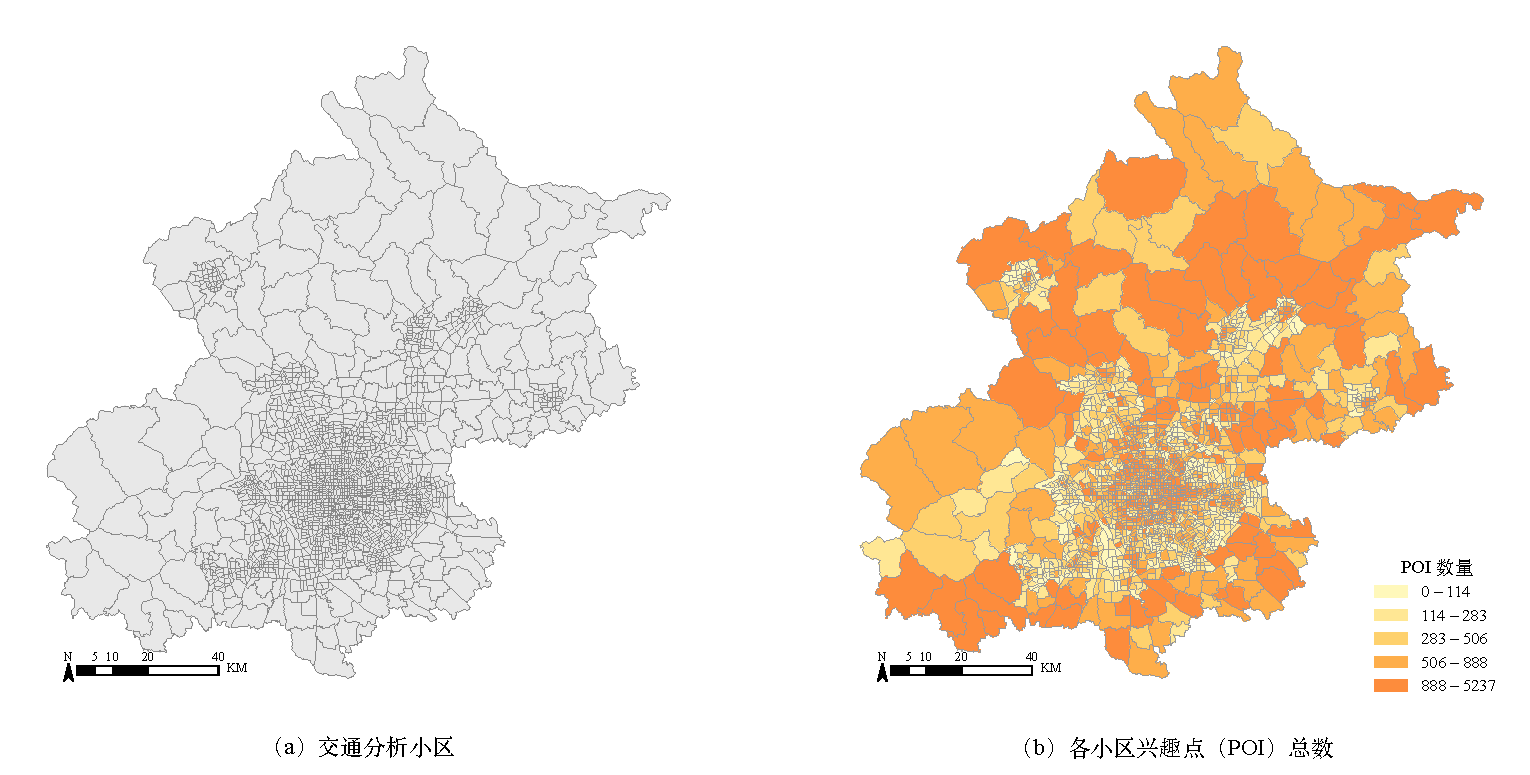
\includegraphics[width=\textwidth]{figures/ch4/zone_poi_cn.pdf}
  \bicaption{北京市交通分析小区与兴趣点空间分布}{Spatial distribution of traffic analysis zones and points of interest in Beijing.}
  \label{fig.cohact.zonepoi}
\end{figure}

\subsection{实验设置与评价指标}\label{subsec.cohact.experiment.setting}

数据划分方面，对预处理后的 32174 户合格家庭，在各行政区内按 9:1 的比例随机划分为训练集与测试集。按行政区分层划分是为使训练集与测试集在空间分布上保持一致，避免因区域人口与出行特征的不均衡而高估或低估模型性能。最终测试集含 3219 户家庭，其 16288 条有效出行作为评价CoHACT模型以及基线模型的测试集。为避免信息泄漏，\ref{sec.cohact.encoder}节中由高斯混合模型聚类得到的活动模式簇以及经蒸馏得到的活动模式预测模型 $g_\phi$均仅在训练集上拟合，随后在训练与推理过程中冻结模型权重，从而确保活动模式先验不携带测试集的信息。

实验环境方面，全部实验基于 PyTorch 实现，运行于配备 13th Gen Intel Xeon i9-13950HX CPU、64\,GB 内存与 24\,GB 显存 NVIDIA RTX 4090 GPU 的个人电脑。CoHACT 的超参数由训练集上的五折交叉验证选取，主要取值见表~\ref{tab.cohact.hyperparam}。训练过程通过模型在验证集上的表现确定最优迭代轮数，并保存对应的模型权重，以避免过拟合。为保证提出的CoHACT模型与其他模型的可比性，后续各基准模型与消融变体均在同一训练集上、以相同的数据预处理与评价指标训练和测试。

{
\small
\begin{longtable}{@{}L{2.7cm}L{8.0cm}C{2.3cm}@{}}
\bicaption{CoHACT 模型超参数设置}{Hyperparameter settings of the CoHACT model.}\label{tab.cohact.hyperparam} \\
\toprule
超参数类型 & 超参数 & 取值 \\
\midrule
\endfirsthead
\multicolumn{3}{l}{\small（续表~\ref{tab.cohact.hyperparam}）}\\
\toprule
超参数类型 & 超参数 & 取值 \\
\midrule
\endhead
\midrule
\multicolumn{3}{r}{\small 续下页}\\
\endfoot
\bottomrule
\endlastfoot

\multicolumn{3}{l}{\textbf{模型结构}} \\*
  & 模型维度 $d_{\mathrm{model}}$        & 256 \\
  & 属性嵌入维度                         & 256 \\
  & 注意力头数                           & 16 \\
  & 编码器 CGC 层数 $L$                  & 2 \\
  & 共享专家数 $m_s$                     & 2 \\
  & 任务专属专家数 $m_k$                 & 2 \\
  & 诱导点数 $n_I$                       & 16 \\
  & 解码器 Transformer 层数 $L_d$        & 16 \\
  & dropout 比率                         & 0.3 \\
\midrule
\multicolumn{3}{l}{\textbf{活动模式与目的地}} \\*
  & 家庭级簇数 $C_h$                     & 20 \\
  & 个人级簇数 $C_p$                     & 40 \\
  & LDA 主题数                           & 12 \\
\midrule
\multicolumn{3}{l}{\textbf{损失函数}} \\*
  & 焦点损失平衡参数 $\alpha$            & 0.25 \\
  & 焦点损失聚焦参数 $\gamma$            & 2.0 \\
\midrule
\multicolumn{3}{l}{\textbf{训练参数}} \\*
  & 优化器                               & AdamW \\
  & 权重衰减                             & $1\times10^{-4}$ \\
  & 初始学习率                           & $5\times10^{-5}$ \\
  & 学习率调度                           & 余弦退火 \\
  & 训练轮数                             & 500 \\
  & 批规模                               & 100 \\
  & 梯度裁剪范数                         & 1.0 \\
\end{longtable}
}

评价指标方面，采用合成人口与活动生成研究中广泛使用的标准化均方根误差（Standardized Root Mean Square Error, SRMSE）度量生成分布与真实分布的差异。SRMSE 通过对真实频率作归一，使不同维度、不同稀疏程度的属性组合上的误差具有可比性，其定义为：
\begin{equation}
\mathrm{SRMSE}=\frac{\sqrt{\dfrac{1}{B}\sum_{b=1}^{B}\bigl(f_b^{\mathrm{gen}}-f_b^{\mathrm{real}}\bigr)^2}}{\dfrac{1}{B}\sum_{b=1}^{B}f_b^{\mathrm{real}}},
\label{eq.cohact.srmse}
\end{equation}
式中，$f_b^{\mathrm{gen}}$ 与 $f_b^{\mathrm{real}}$ 分别为生成活动计划与真实活动计划落入交叉分类属性空间第 $b$ 个区间的相对频率，$B$ 为区间总数；SRMSE 越小，表示生成分布与真实分布越接近，取零时说明生成分布与真实分布完全一致。

由于本章关注的是家庭级活动计划生成，单一维度的 SRMSE 不足以全面刻画家庭级活动计划的生成质量，故从个体与家庭两个层面，由简到繁地计算多维度的 SRMSE。在个体层面，构造四个逐步纳入更多属性的维度子集：4D 子集涵盖出发时间、到达时间、出发地与目的地四项时空属性，刻画活动的时空属性；5D-purpose 与 5D-mode 子集在 4D 子集的基础上分别加入活动目的与出行方式，考察模型对行为属性的还原能力；8D-full 子集进一步纳入联合出行与驾驶标识，构成包含全部属性的最严格联合分布。随属性维度增加，交叉分类下的属性组合数迅速膨胀、对联合分布还原能力的要求也随之提高，因而由 4D 至 8D-full 的 SRMSE 变化可反映模型在高维联合分布上的稳健性。此外，单独计算剔除出发地与目的地的 6D 子集（即 8D-full 去除出发地与目的地属性），以评估非空间属性的拟合质量，从而间接评估目的地注意力层对空间维度的生成质量。

在家庭层面，为检验模型是否真正再现了家庭内部活动计划的协调结构，将活动计划按家庭聚合为五项家庭活动计划统计量，即家庭总出行数、联合出行比例、主导出行方式、主导活动目的与不同目的地数，并计算其交叉分布的 Household-SRMSE。该指标从家庭整体视角度量生成结果与真实调查的差异，与个体级 SRMSE 互补，共同构成对家庭级活动计划生成质量的多维度评价体系。

\subsection{基准模型对比分析}\label{subsec.cohact.experiment.baseline}

由于目前尚无专为家庭级活动计划生成而设计的深度生成模型，本小节选取合成人口与活动生成研究中广泛采用的六个代表性深度生成模型作为基准。其中，生成对抗网络（Generative Adversarial Network, GAN）、Wasserstein GAN（WGAN）与变分自编码器（Variational Autoencoder, VAE）为非条件生成模型，直接学习活动-出行属性的联合分布；在此基础上，进一步引入它们以家庭与成员属性为条件输入的条件版本（CGAN、CWGAN、CVAE），以考察显式条件信息对生成质量的影响。

上述基准模型涵盖对抗式与变分式两大类主流生成范式及其条件化变体，能够较为全面地代表既有方法在该任务上的水平。为使性能差异归因于模型设计而非模型参数规模，所有基准模型均在同一训练集上以相同的优化器设置与学习率训练，并配置与 CoHACT 相近的参数量。需要指出的是，这些基准均沿用既有研究将居民视作彼此独立样本的建模方式，缺乏对家庭内部活动计划协调的显式刻画，因而与本章方法的对比可直接反映家庭级活动计划协调建模所带来的价值。

表~\ref{tab.cohact.baseline} 给出 CoHACT 与六个基准模型在五个SRMSE子集及家庭层面SRMSE的多维度对比。总体来看，CoHACT 在全部子集、个体与家庭两个层面均显著优于全部六个基准模型，且其性能优势远超基准模型之间的性能差异，表明该性能提升来自模型本身的改进而非参数微调。

{
\small
\setlength{\tabcolsep}{3pt}
\begin{longtable}{@{}L{2.0cm}*{5}{C{1.7cm}}C{2.0cm}@{}}
\bicaption{CoHACT 与基准模型的多维度 SRMSE 对比（值越小越优，最优模型以加粗标出）}{Comparison of multidimensional SRMSE values between CoHACT and the baseline models (lower values indicate better performance; the best-performing model is shown in bold).}\label{tab.cohact.baseline} \\
\toprule
模型 & \makecell{SRMSE\\(4D)} & \makecell{SRMSE\\(5D-\\purpose)} & \makecell{SRMSE\\(5D-mode)} & \makecell{SRMSE\\(8D)} & \makecell{SRMSE\\(6D)} & \makecell{Household-\\SRMSE} \\
\midrule
\endfirsthead
\multicolumn{7}{l}{\small（续表~\ref{tab.cohact.baseline}）}\\
\toprule
模型 & \makecell{SRMSE\\(4D)} & \makecell{SRMSE\\(5D-\\purpose)} & \makecell{SRMSE\\(5D-mode)} & \makecell{SRMSE\\(8D)} & \makecell{SRMSE\\(6D)} & \makecell{Household-\\SRMSE} \\
\midrule
\endhead
\midrule
\multicolumn{7}{r}{\small 续下页}\\
\endfoot
\bottomrule
\endlastfoot

GAN   & 52.21 & 53.54 & 53.19 & 54.52 & 15.46 & 3.71 \\
WGAN  & 55.08 & 56.57 & 56.18 & 57.67 & 17.40 & 3.88 \\
VAE   & 52.80 & 54.17 & 53.80 & 55.17 & 13.95 & 4.30 \\
CGAN  & 28.91 & 29.57 & 29.41 & 30.06 &  8.27 & 4.63 \\
CWGAN & 31.55 & 32.27 & 32.11 & 32.83 &  9.46 & 4.32 \\
CVAE  & 31.66 & 32.41 & 32.22 & 32.95 &  8.31 & 4.17 \\
\midrule
CoHACT & \textbf{1.69} & \textbf{1.82} & \textbf{1.86} & \textbf{1.95} & \textbf{4.31} & \textbf{1.48} \\
\end{longtable}
}

具体到个体层面，CoHACT 将最严格的 8D-full 子集的 SRMSE 降至 1.95，约为最优基准模型（CGAN，30.06）的 $1/15$、最差基准模型（WGAN，57.67）的近 $1/30$；在 4D、5D-purpose 与 5D-mode 子集上同样保持 1.69\,\textasciitilde\,1.86 的较好性能，超越各基准模型一个数量级以上。值得关注的是，生成误差随属性维度呈现出逐渐增长的趋势，即，各基准模型的 SRMSE 由 4D 到 8D-full 持续上升（如 WGAN 由 55.08 升至 57.67、CGAN 由 28.91 升至 30.06），反映出在逐步纳入活动目的、出行方式、联合与驾驶标识后，问题的复杂度增加导致模型联合分布还原能力的下降；相比之下，CoHACT 由 4D 到 8D-full 仅由 1.69 微增至 1.95，几乎不随维度恶化。这一稳健性源于本章解码器以多任务注意力网络逐属性建模、并以自回归方式沿活动计划联合生成全部属性，使高维属性间的依赖得以保持。

进一步讨论个体层面CoHACT模型的优势，在移除出发地与目的地预测的 6D 子集上，CoHACT（4.31）虽仍最优，但其相对基准模型（8.27\,\textasciitilde\,17.40）的差距明显小于含空间预测的子集。与之相对，一旦将出发地与目的地纳入评价维度，基准模型的误差便急剧上升——以 GAN 为例，其 SRMSE 由 6D 子集的 15.46 陡增至 8D-full 的 54.52，VAE、WGAN 等模型也呈现出相同的模式。这一模式说明，城市尺度下的目的地选择是基准模型误差的主要来源，也正是 CoHACT 优势最为显著的环节。在数千个候选交通小区构成的大规模候选集上，基准模型因缺乏有效的空间建模机制而损失大量精度，CoHACT 则凭借目的地注意力层将空间预测误差控制在较低水平，从而间接验证了该层的有效性（其贡献将在\ref{subsec.cohact.experiment.ablation}小节的消融实验中进一步讨论）。

在家庭层面，CoHACT 的 Household-SRMSE 为 1.48，仍全面优于基准模型，约为最优基准（GAN，3.71）的 40\%、最差基准（CGAN，4.63）的 $1/3$。值得注意的是，家庭层面CoHACT性能优势小于个体层面，其原因在于 Household-SRMSE 所聚合的五项家庭统计量（总出行数、联合出行比例、主导出行方式、主导活动目的与不同目的地数）中，多数特征可由个体级别边际分布近似还原，基准模型在这些维度上本已能取得尚可的匹配，故 CoHACT 的提升空间相对受限。即便如此，1.48 的 Household-SRMSE 仍较各基准降低逾一半，说明本章的家庭协调式解码器与纳什议价协调层不仅保证了个体属性的真实，也使家庭整体统计更贴近真实的家庭级活动计划。

此外，条件生成模型和非条件生成模型在个人和家庭层面上表现出的性能差异也值得关注。在个体层面的性能评估中，三个条件基准模型（CGAN、CWGAN、CVAE）的 SRMSE 显著优于其对应的非条件版本（如 8D-full 子集上 CGAN 的 30.06 远低于 GAN 的 54.52），说明以家庭与成员属性为条件输入确实能压缩生成空间、改善个体边际分布的匹配。然而，这一性能改善并未出现在家庭层面的评估中。三个条件模型的 Household-SRMSE 介于 4.17\,\textasciitilde\,4.63，略差于非条件模型的 3.71\,\textasciitilde\,4.30。上述个人层面与家庭层面性能的差异表明，仅将家庭属性作为条件输入，本身并不足以诱导生成合理的家庭级活动计划。究其原因，条件基准模型虽共享了家庭背景信息，但仍在各成员之间相互独立地采样，缺乏对成员间车辆共享、联合出行与接送等耦合关系的显式建模，故条件信息带来的改善仅停留在个体边际层面，甚至可能因强化独立采样下的个体最优而加剧家庭层面的不一致。这恰从反面印证了本章在解码器中引入跨角色注意力、并以纳什议价协调层显式建模家庭内部耦合的必要性。

\subsection{消融实验分析}\label{subsec.cohact.experiment.ablation}

为进一步识别 CoHACT 中关键组件的贡献，考虑到编码器与解码器是活动链生成的主干，移除任一者都将使模型无法产出完整的活动计划，故本小节仅对基于纳什议价的家庭活动计划协调层与考虑空间异质性的目的地注意力层进行消融实验分析。考虑到计算开销与消融的可解释性，每次消融实验从完整模型中移除一个组件，共计形成三种模型结构：CoHACT（完整模型）、CoHACT w/o Nash（移除基于纳什议价的家庭活动计划协调层）与 CoHACT w/o spatial（移除考虑空间异质性的目的地注意力层）。

表~\ref{tab.cohact.ablation} 给出三种模型配置在五个个人级属性子集上的 SRMSE 与 Household-SRMSE。总体而言，完整 CoHACT 在多数子集与家庭层面均取得最优，而两个组件的移除分别在不同维度上引起性能退化。

{
\small
\setlength{\tabcolsep}{3pt}
\begin{longtable}{@{}L{2.8cm}*{5}{C{1.7cm}}C{2.0cm}@{}}
\bicaption{消融实验结果（最优模型以加粗标出）}{Results of ablation experiments (the best-performing model is shown in bold).}\label{tab.cohact.ablation} \\
\toprule
配置 & \makecell{SRMSE\\(4D)} & \makecell{SRMSE\\(5D-\\purpose)} & \makecell{SRMSE\\(5D-mode)} & \makecell{SRMSE\\(8D)} & \makecell{SRMSE\\(6D)} & \makecell{Household-\\SRMSE} \\
\midrule
\endfirsthead
\multicolumn{7}{l}{\small（续表~\ref{tab.cohact.ablation}）}\\
\toprule
配置 & \makecell{SRMSE\\(4D)} & \makecell{SRMSE\\(5D-\\purpose)} & \makecell{SRMSE\\(5D-mode)} & \makecell{SRMSE\\(8D)} & \makecell{SRMSE\\(6D)} & \makecell{Household-\\SRMSE} \\
\midrule
\endhead
\midrule
\multicolumn{7}{r}{\small 续下页}\\
\endfoot
\bottomrule
\endlastfoot

CoHACT      & 1.69 & \textbf{1.82} & \textbf{1.86} & \textbf{1.95} & 4.31 & \textbf{1.48} \\
CoHACT w/o Nash     & \textbf{1.67} & 2.02 & 2.00 & 2.14 & 5.62 & 2.18 \\
CoHACT w/o spatial  & 1.98 & 2.10 & 2.12 & 2.22 & \textbf{3.81} & 1.70 \\
\end{longtable}
}

首先，移除基于纳什议价的家庭活动计划协调层后，模型在4D 子集上的性能基本不变（1.67 对 1.69），甚至性能表现略有提升，但在其余子集上的性能均明显变差，尤其是不预测出发地与目的地的 6D 子集（由 4.31 升至 5.62）与家庭层面的 Household-SRMSE（由 1.48 升至 2.18）。移除基于纳什议价的家庭活动计划协调层后的性能变化与该层的作用机理高度吻合。针对4D 子集，纳什议价层经近端正则项使协调解整体贴近解码器输出，且纳什议价协调层要求的联合活动的时间与空间异质性仅针对小部分联合出行成员，对 4D 整体分布的净扰动较小。正因纳什议价协调层以极小的边际拟合代价换取成员间的时间一致，移除该层后时间的边际拟合反而回到解码器的最优，使 4D 略有改善。与之相对，性能退化集中于 6D 子集与 Household-SRMSE，原因分析如下：6D 子集相较 4D 子集额外纳入出行方式、联合出行与驾驶等行为属性，正是纳什议价层经车辆可用性约束与联合一致性约束（耦合成员间的方式与联合出行）最直接重塑的对象，而Household-SRMSE所聚合的指标也是家庭层面的协调结果，是纳什议价层主要施加约束的对象。因此，去掉纳什议价协调层后，家庭内部的行为协调与可行性显著下降，导致 6D 子集与 Household-SRMSE 的性能恶化。换句话说，纳什议价层以个体边际拟合的微小让步，换取了家庭内部行为协调与可行性的显著改善。

另外，移除考虑空间异质性的目的地注意力层后，模型的性能变化呈现出与移除纳什议价层近乎相反的模式：所有含出发地和目的地预测的子集均显著变差（如 4D 由 1.69 升至 1.98、8D-full 由 1.95 升至 2.22、Household-SRMSE 由 1.48 升至 1.70），而无出发地和目的地预测的 6D 子集反而略有改善（由 4.31 降至 3.81）。这一``跷跷板''的现象源于多任务学习中任务间的梯度竞争。当解码器须同时承担目的地选择与其余属性预测时，规模庞大的目的地任务会主导模型的梯度更新，使模型在空间属性上拟合更优；一旦移除该任务，模型得以将训练重点集中于非空间属性，故 6D 子集的拟合反而更优，但损失了对城市尺度目的地预测的能力，使所有含出发地与目的地预测的空间精度明显下降。

综合来看，上述消融结果一方面验证了两个组件的贡献，另一方面也解释了CoHACT能在各维度上取得良好表现的原因。纳什议价层与目的地注意力层分别补足了基准模型在家庭活动计划协调与空间精度这两方面的短板，且二者作用维度近乎正交、互不干扰，故同时保留时，模型既能维持较好的空间预测精度、又能保证家庭级活动计划的协调与可行性。需要补充的是，本小节以 SRMSE 度量的是分布层面的模型性能，而纳什议价层对车辆可用性等硬约束的严格保障难以由分布指标完全体现，这一点将在\ref{subsec.cohact.experiment.coord}小节通过家庭级活动计划内部协调性的分析进一步检验。

\subsection{家庭级活动计划内部协调性}\label{subsec.cohact.experiment.coord}

与基准模型的多维度 SRMSE 对比实验已表明 CoHACT 在个体活动计划与家庭活动计划两个层面均取得远优于基准模型的性能，但 SRMSE 主要刻画生成的属性分布与实际分布的吻合程度，不能直接回答``生成的家庭级活动计划是否真正合理''这一问题。为此，本小节从车辆共享、联合出行、接送行为等角度选取六项刻画生成的家庭级活动出行计划特征的指标，主要分为两类：一类关注家庭活动计划的可行性，即驾驶人数与家庭车辆数的匹配；另一类关注家庭成员在活动安排上的相互配合程度，包括联合出行与接送等协调行为以及亲子在外时间的重叠。将 CoHACT 生成的家庭级活动计划与实际的家庭级活动计划逐一比较，对比结果如图~\ref{fig.cohact.coord} 所示。

\begin{figure}[H]
  \centering
  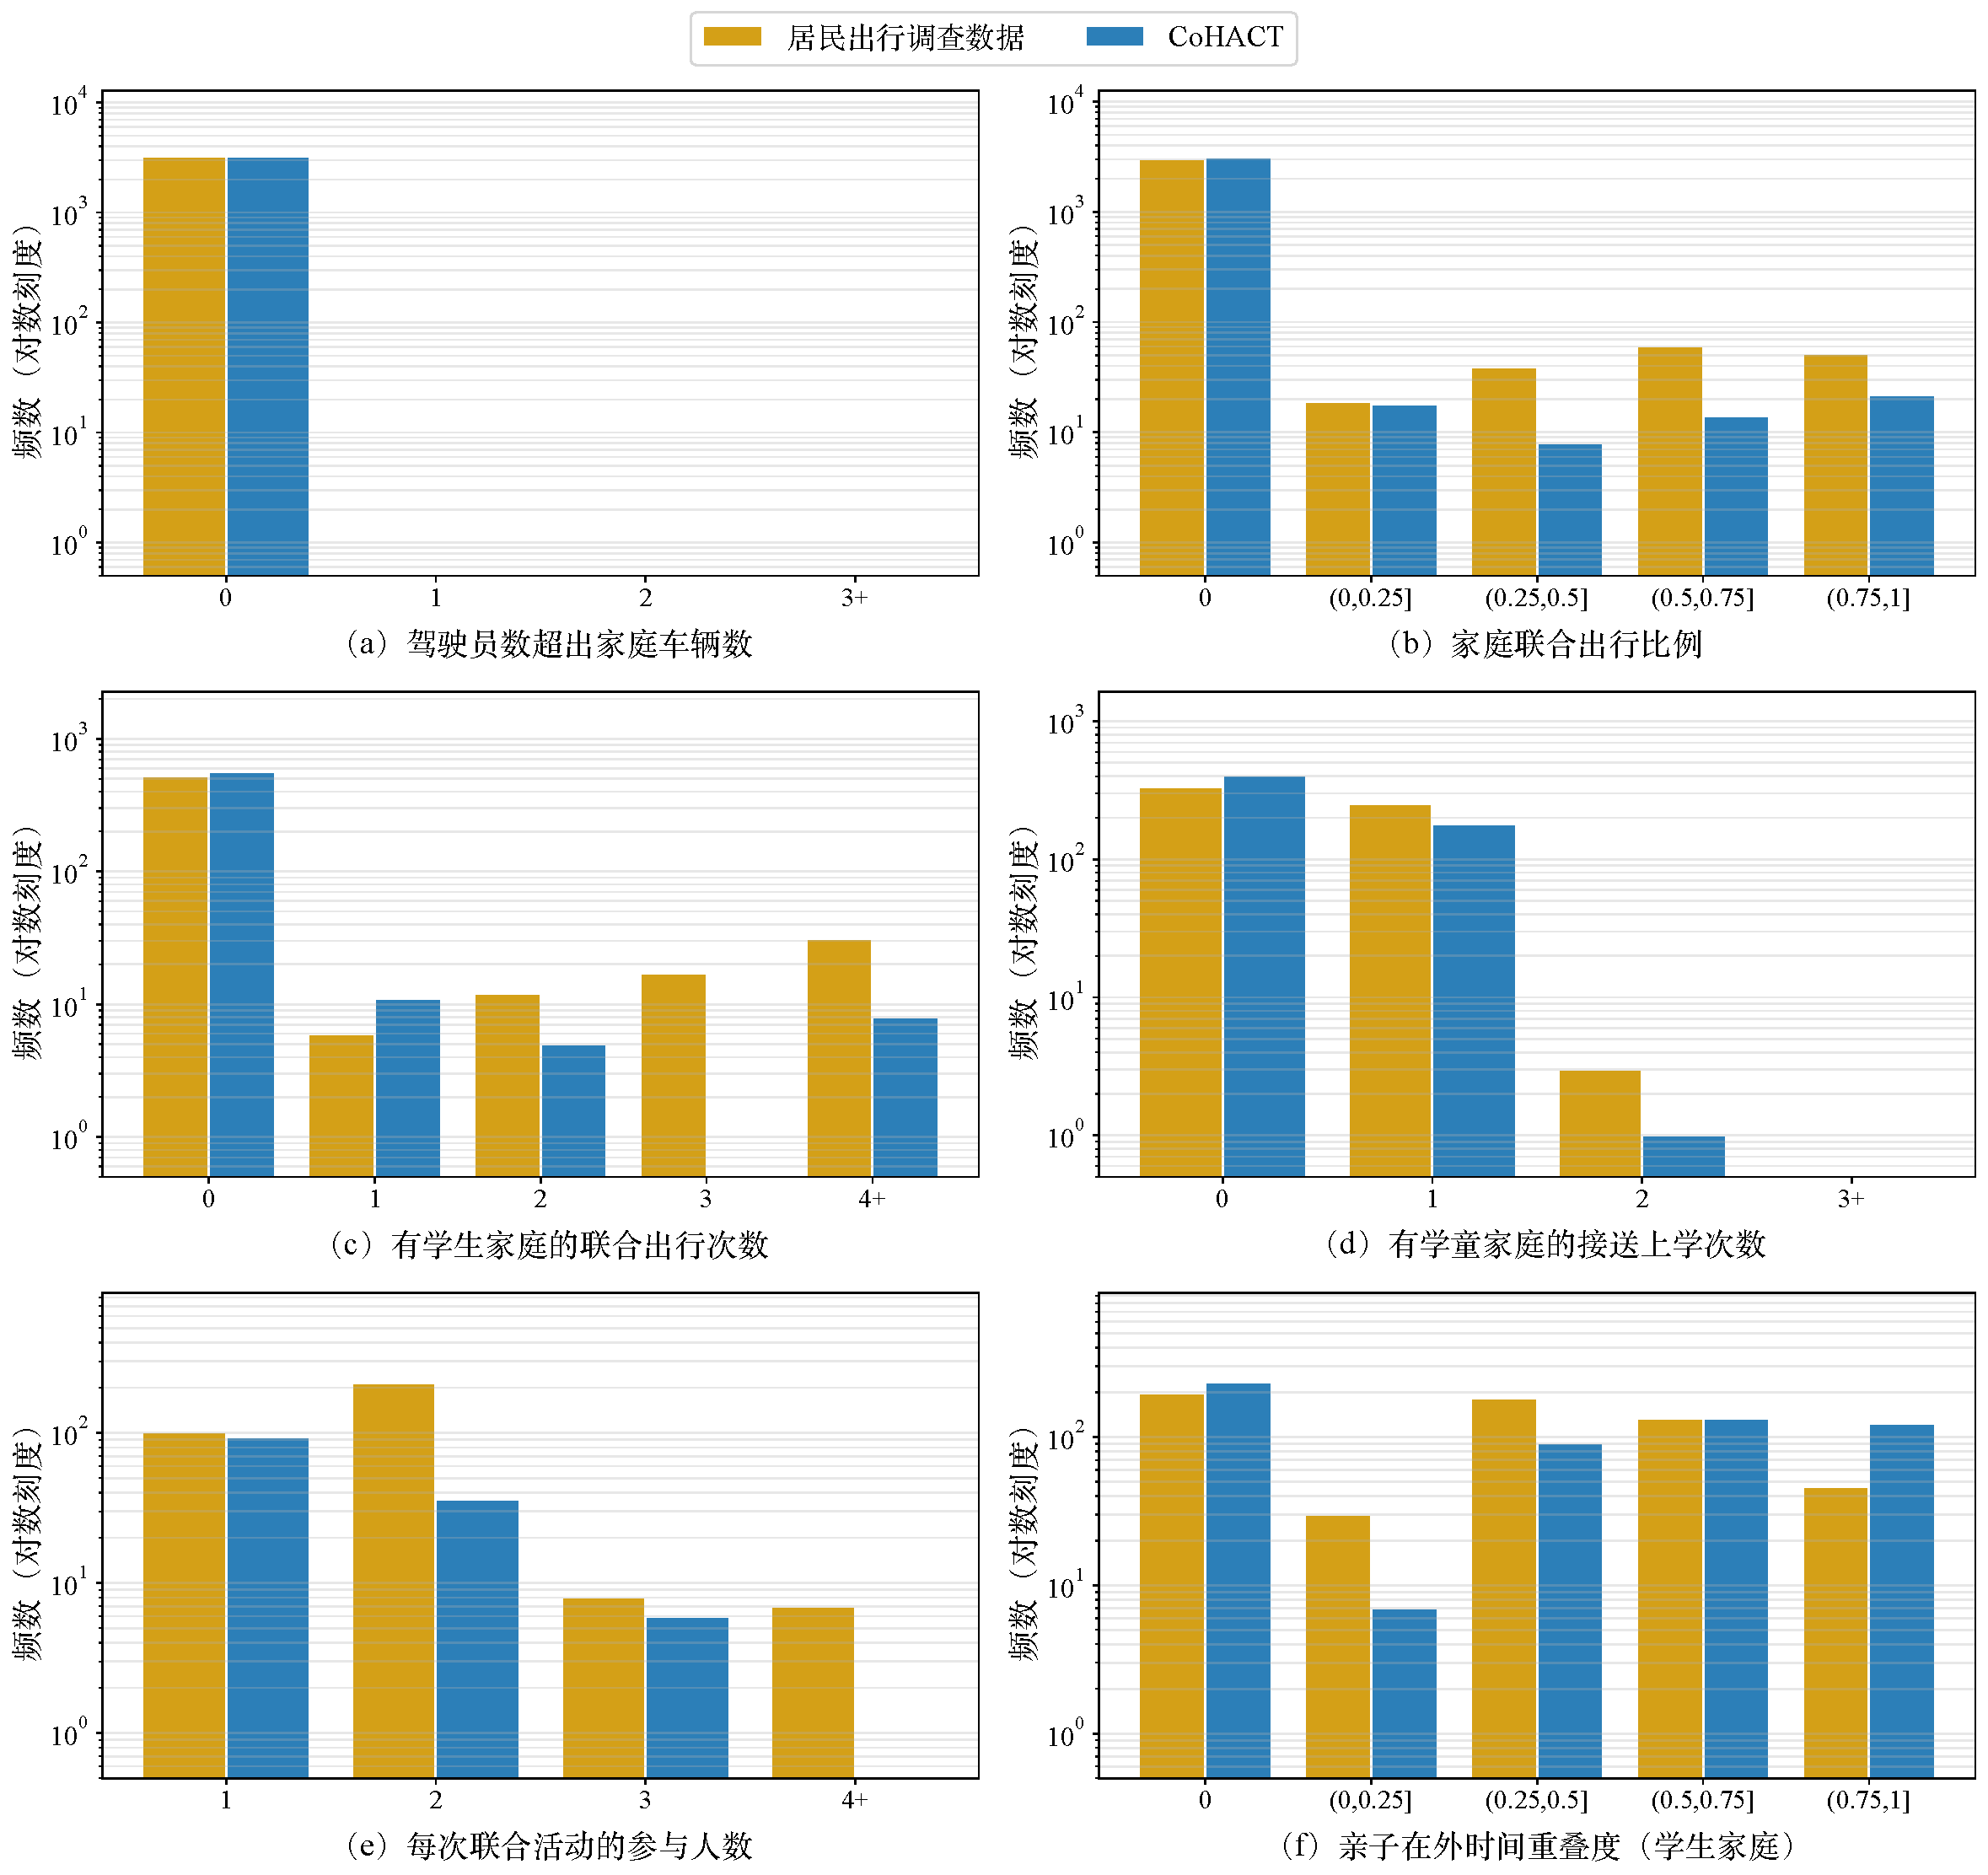
\includegraphics[width=\textwidth]{figures/ch4/family_coord_distributions_log_cn.pdf}
  \bicaption{CoHACT 生成家庭级活动计划与实际分布对比}{Comparison of household-level activity chain between CoHACT-generated and observed data.}
  \label{fig.cohact.coord}
\end{figure}

在家庭级活动计划的可行性方面，选取统一家庭中同时驾车出行的成员数是否超过家庭车辆数作为指标（即是否存在车辆超配），刻画家庭车辆资源分配的可行性。如图~\ref{fig.cohact.coord}(a) 所示，全部 3219 户生成的家庭活动计划均不存在车辆超配情况，与实际的家庭级活动计划完全一致，符合家庭车辆资源约束的硬性要求。上述生成的家庭级活动计划并无车辆超配的结果证明了基于纳什议价的家庭活动计划协调层的有效性。具体而言，作为对照，CoHACT模型在移除纳什议价层后，存在车辆超配的家庭活动计划的占比升高至 17.3\%。因此，基于纳什议价的家庭活动计划协调层是 CoHACT 保证家庭级活动计划可行性的关键所在，其通过满足家庭级的资源约束，确保了生成的家庭级活动计划的合理性。

在联合出行与接送行为方面，相应指标整体拟合情况良好，但存在一定程度的不匹配。如图~\ref{fig.cohact.coord}(b)\,\textasciitilde\,(e) 所示，相较于实际的家庭活动计划，CoHACT 模型生成了较多的具有少量联合出行与接送的家庭，低估了联合出行与接送较频繁的家庭数量。与之相反，图~\ref{fig.cohact.coord}(f) 中，CoHACT生成了较多的亲子在外时间重叠度较高的家庭。以上指标的不匹配的成因与联合出行行为本身的稀疏性有关。在实际的居民出行调查中，频繁开展联合出行与接送的家庭本属少数，\ref{sec.cohact.loss}节的焦点损失虽已在一定程度上缓解了类别不平衡，但自回归生成与纳什议价协调层仍倾向于产生较为保守的联合出行与接送水平，从而在生成的家庭级活动计划中略低估了联合出行与接送行为的强度。尽管如此，模型再现了各项指标分布的整体形态，说明 CoHACT 已能以合理精度刻画家庭的联合出行与接送行为。

综上，家庭级活动计划内部协调性的分析从具体的家庭联合活动层面印证了 SRMSE 所反映的家庭级优势：一方面，CoHACT生成的家庭级活动计划严格遵守车辆共享这一家庭资源约束，与实际的家庭活动出行计划完全一致，凸显了纳什议价协调层在保证可行性上的有效性；另一方面，虽略有保守，但CoHACT模型可以较好地再现联合出行与接送等行为。这表明 CoHACT 生成的家庭活动计划不仅在分布统计上贴近真实调查的结果，也在家庭联合活动协调的行为机制上具备一定的可信度。

\subsection{个体级活动计划属性分布}\label{subsec.cohact.experiment.dist}

在确认CoHACT模型能够生成较为可信的家庭级活动计划的基础上，进一步考察生成的样本是否同时保持了个体级活动计划的属性分布。为此，将生成的个体活动计划与实际的个体活动计划在六个属性（出发地与目的地除外）的一维边际分布上逐一比较（图~\ref{fig.cohact.marginals}），并进一步比较以上属性衍生的出行距离分布（图~\ref{fig.cohact.triplength}）和活动时长分布（图~\ref{fig.cohact.duration}），以检验生成样本在个体级活动计划属性分布上的真实性。

\begin{figure}[H]
  \centering
  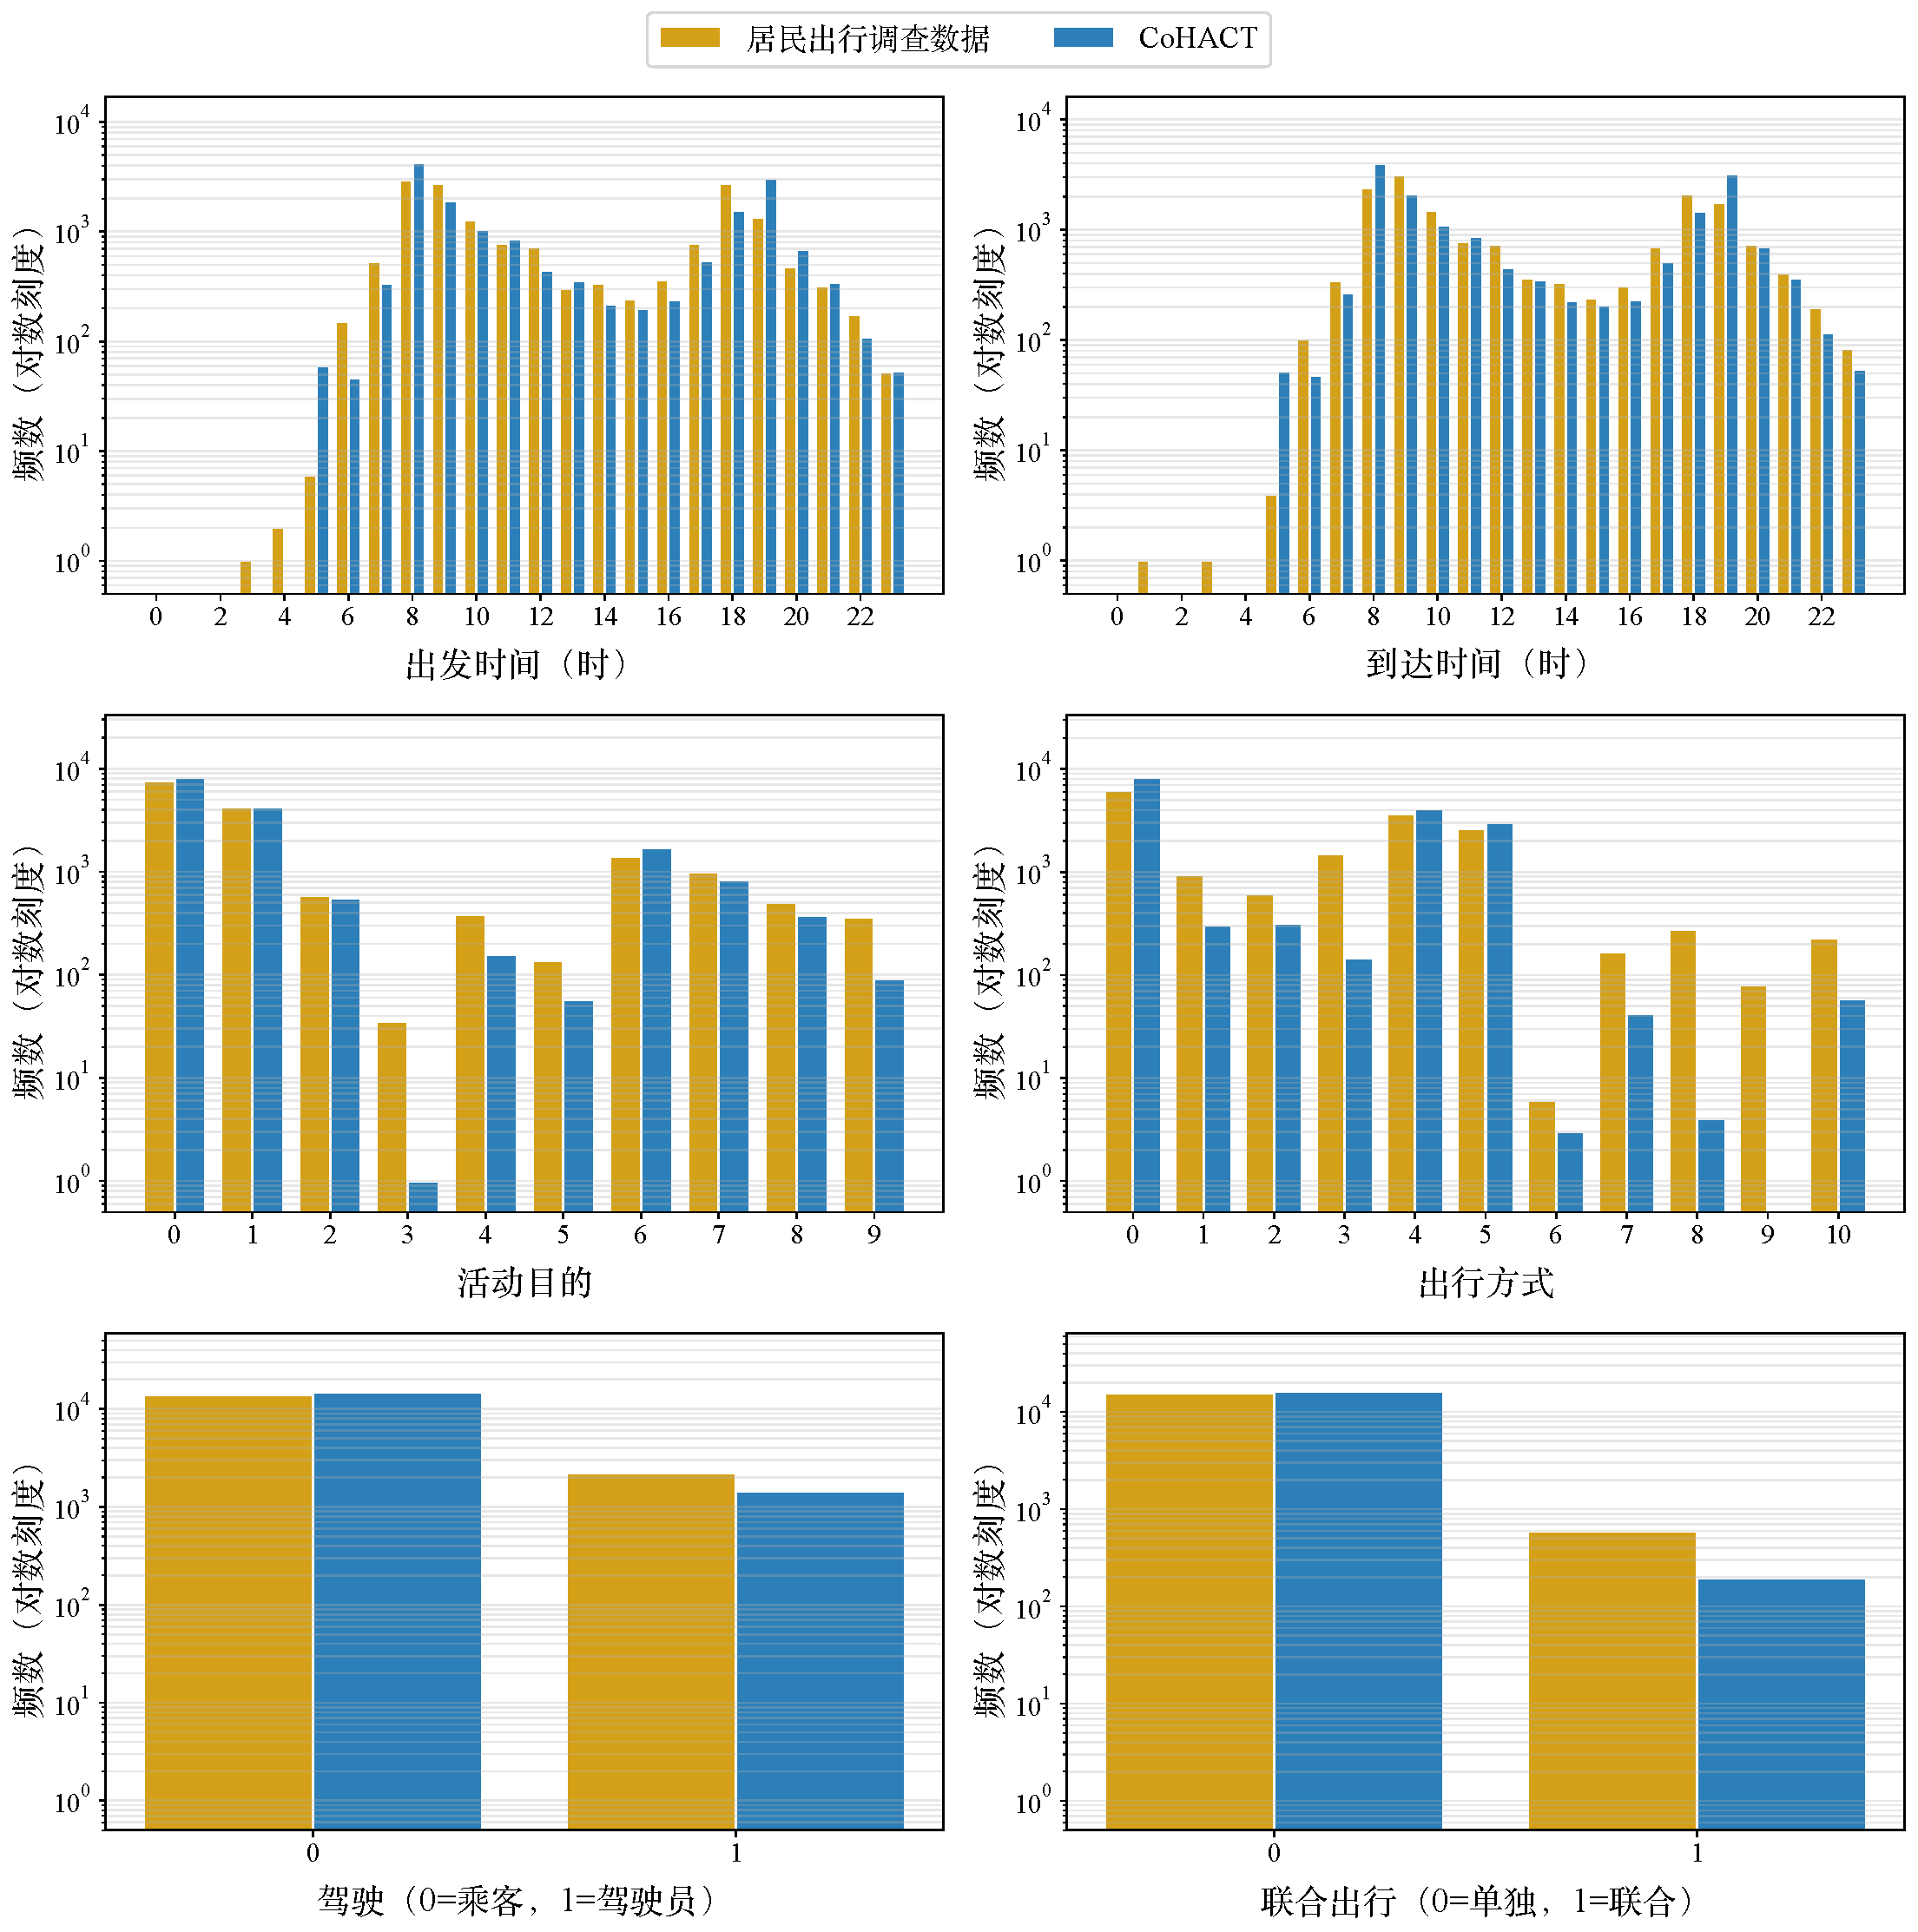
\includegraphics[width=\textwidth]{figures/ch4/marginals_6attr_cn.pdf}
  \bicaption{CoHACT 生成的活动计划与实际活动计划的一维边际分布对比}{Comparison of one-dimensional marginal distributions between activity chains generated by CoHACT and observed activity chains.}
  \label{fig.cohact.marginals}
\end{figure}

图~\ref{fig.cohact.marginals} 的六个子图表明，生成活动计划与实际的活动计划在在这六个属性的边际分布上高度吻合。在时间属性上，出发时间与到达时间子图显示 CoHACT 准确再现了居民的一日的出行节律，尤其是早高峰与晚高峰构成的双峰形态。在活动目的、出行方式、是否为驾驶员与是否为联合出行四个类别属性上，CoHACT模型生成的活动计划能够复现实际活动计划的主要类别分布。以活动目的为例，最为频繁出现的类别分布匹配情况良好，第二频繁出现类别的计数完全一致，但在部分少数类别上的拟合效果欠佳。其成因同样在于数据分布的不平衡，即，主导类别样本数量更多，模型在优化总体损失时更侧重对其拟合，尽管\ref{sec.cohact.loss}节已引入焦点损失以提升出现频次较低的类别的权重，但稀有活动类型、出行方式等稀疏类别的再现仍是活动生成中的公认难题。总体而言，尽管CoHACT生成的样本在部分稀有属性上的拟合效果欠佳，但仍能较好地再现个体级活动计划的属性的整体分布。

在出行距离与活动时长方面，生成的活动计划与实际活动计划的分布拟合情况也比较良好。图~\ref{fig.cohact.triplength} 显示生成的活动计划再现了真实出行距离分布的右偏形态与长尾特征，二者整体贴合，说明模型能够刻画出行距离短途为主、长途偶发的一般规律。两分布的主要差异在于极短距离处模型将过多出行集中于 1\,km 以下，这与目的地选择中地理阻抗惩罚有关，即，阻抗惩罚在抑制不合理的长距离出行的同时，也使生成的目的地略向出发地的邻近区域集中，从而导致模型在一定程度上倾向于生成极短距离的出行。

\begin{figure}[H]
  \centering
  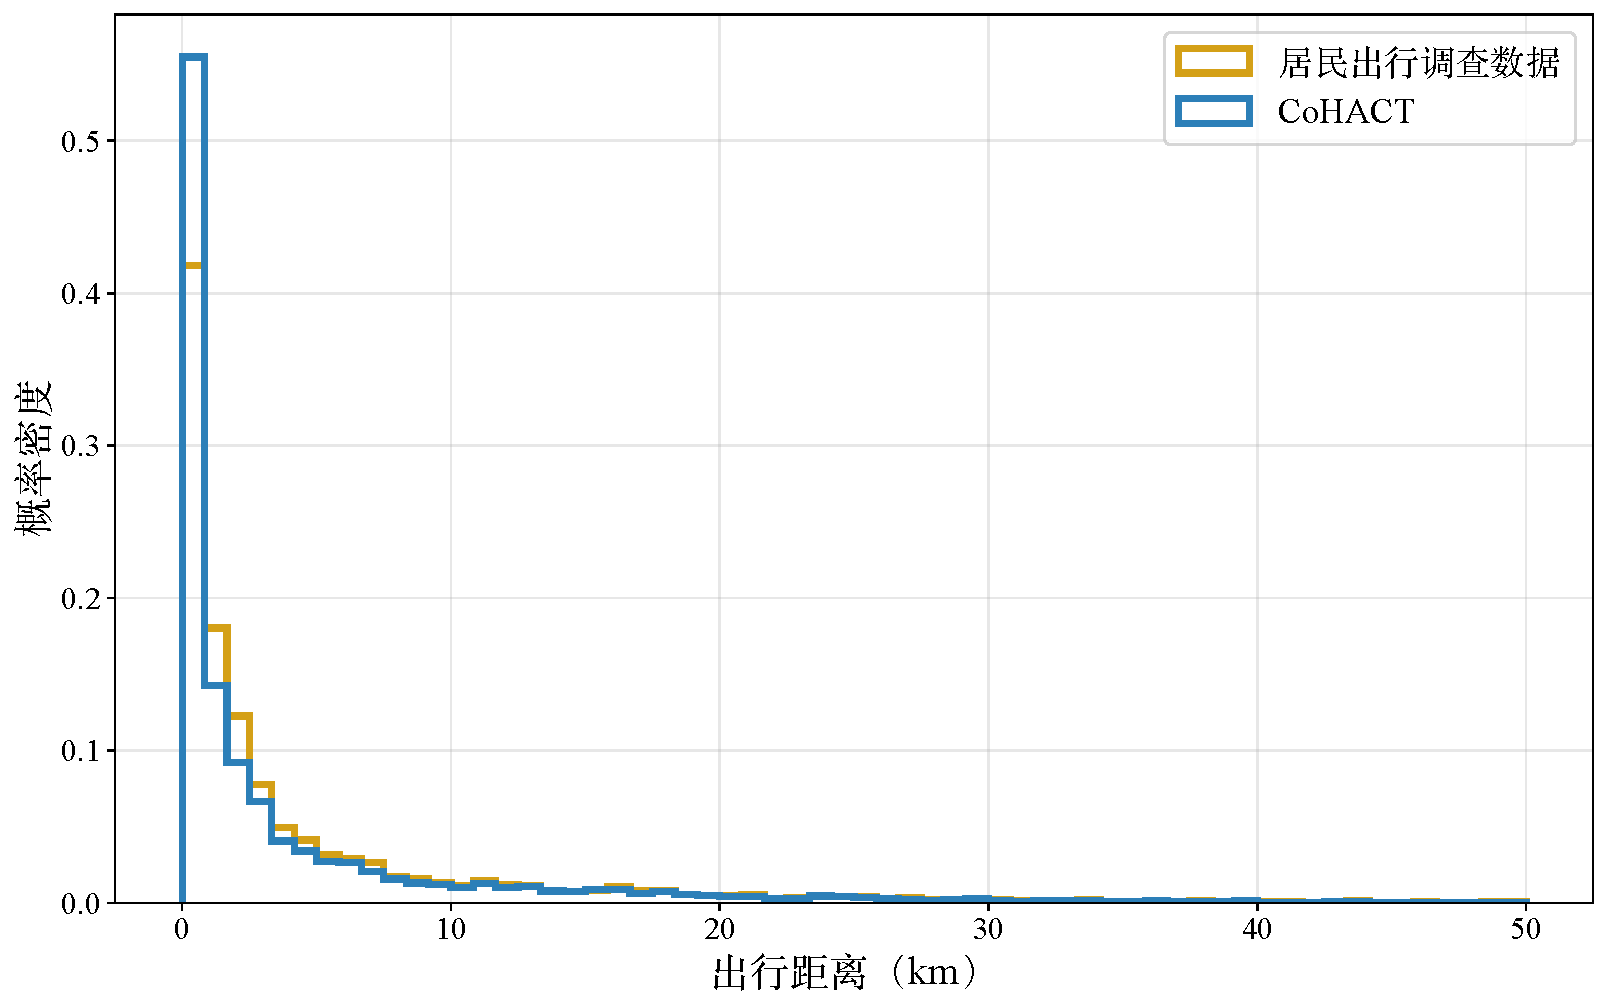
\includegraphics[width=0.85\textwidth]{figures/ch4/trip_length_cn.pdf}
  \bicaption{真实调查与 CoHACT 生成样本的出行距离分布}{Comparison of trip-distance distributions between household travel survey data and samples generated by CoHACT.}
  \label{fig.cohact.triplength}
\end{figure}

在活动时长方面，图~\ref{fig.cohact.duration} 显示 CoHACT 生成的活动计划再现了真实分布的总体形态，如约1小时左右的较短的活动时长峰值、接近工作时长的较长活动时长峰值。需要注意的是，生成分布的长活动峰约后移 1 小时且更为集中，即，模型峰值约在 11 小时，而真实分布峰值约在 9\,\textasciitilde\,10 小时。这一偏移与出发时间、到达时间子图中略微右偏的晚高峰相互呼应。较晚的返回时刻意味着更长的在外活动时长，二者在逻辑上自洽，说明该偏差并非随机噪声，而是源于时间属性生成上的轻微后移。除这一偏移外，两个分布在活动时长分布上整体贴合良好。

\begin{figure}[H]
  \centering
  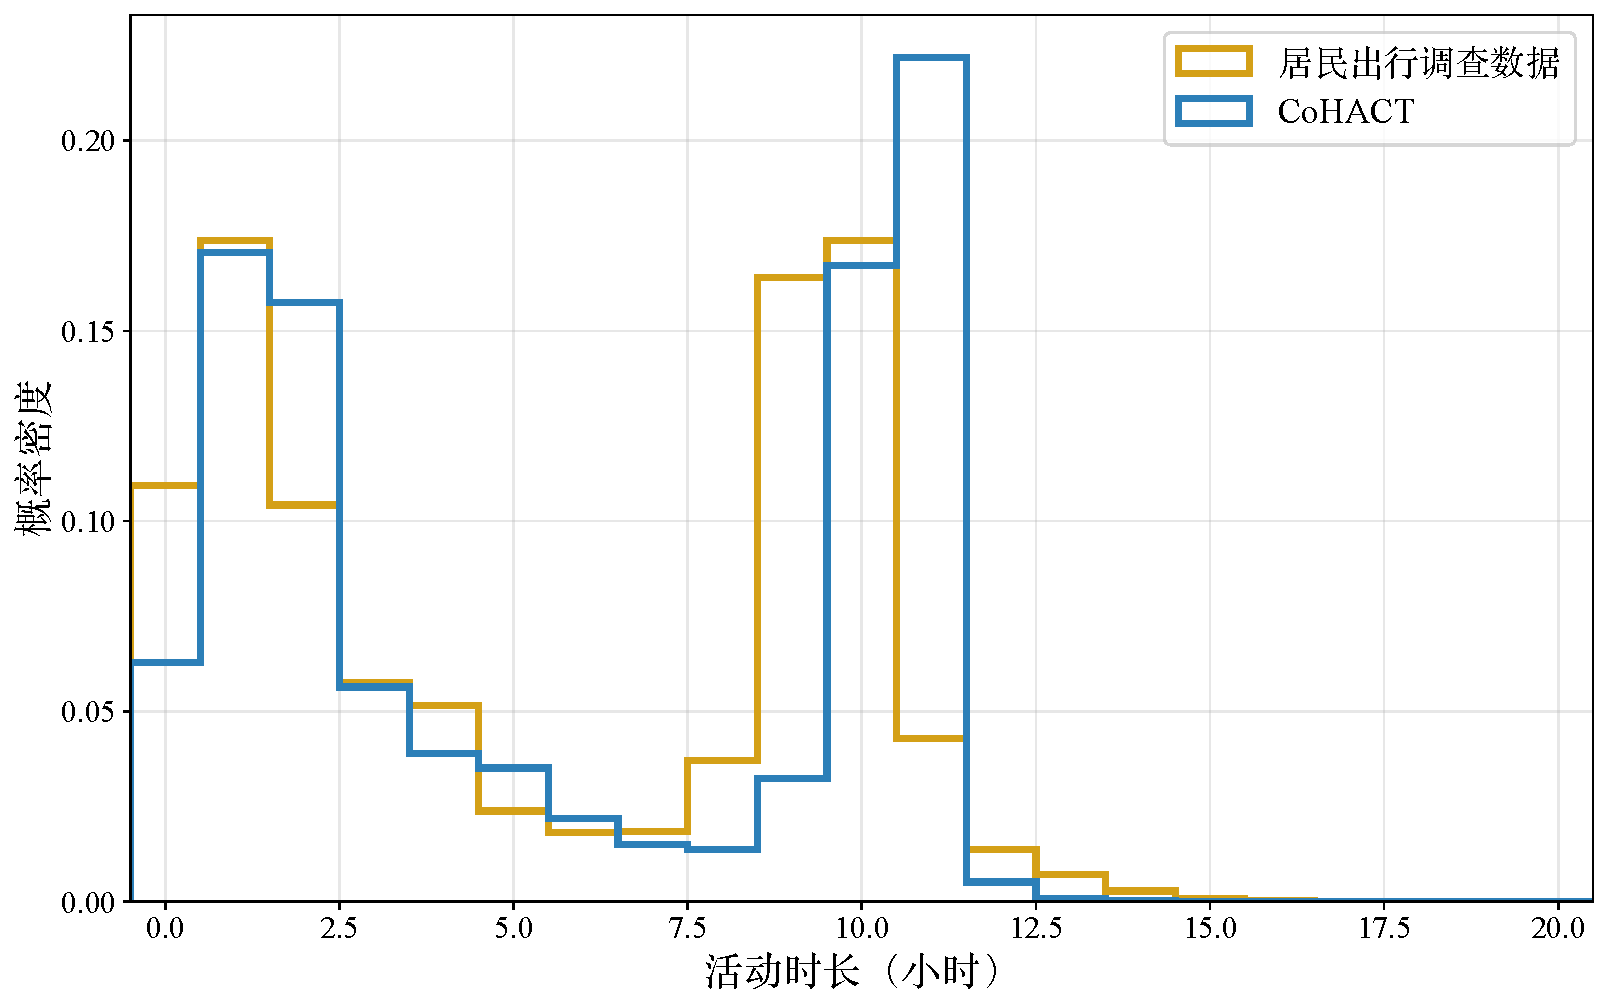
\includegraphics[width=0.85\textwidth]{figures/ch4/duration_cn.pdf}
  \bicaption{真实调查与 CoHACT 生成样本的活动时长分布}{Comparison of activity-duration distributions between household travel survey data and samples generated by CoHACT.}
  \label{fig.cohact.duration}
\end{figure}

综合图~\ref{fig.cohact.marginals}、图~\ref{fig.cohact.triplength} 与图~\ref{fig.cohact.duration} 的对比可见，CoHACT 在保证家庭级活动计划合理性的同时并未牺牲生成的活动计划在个体属性与真实分布的拟合度，说明模型在家庭级与个体级两个层面均能生成较为真实的活动计划。

\subsection{目的地空间分布}\label{subsec.cohact.experiment.spatial}

基准模型的效果对比侧面说明了CoHACT模型在目的地选择上具有显著优势，但并未直接验证CoHACT生成的目的地分布到底是否与实际的目的地分布相符。为检验 CoHACT 中目的地注意力层的有效性，进一步检验生成目的地的空间精度。为此，在全市的 2006 个交通小区上将生成样本的目的地分布与真实数据的目的地分布进行比较。首先，绘制两者的空间分布图，并计算二者的频率之差，结果如图~\ref{fig.cohact.choropleth} 所示。

\begin{figure}[H]
  \centering
  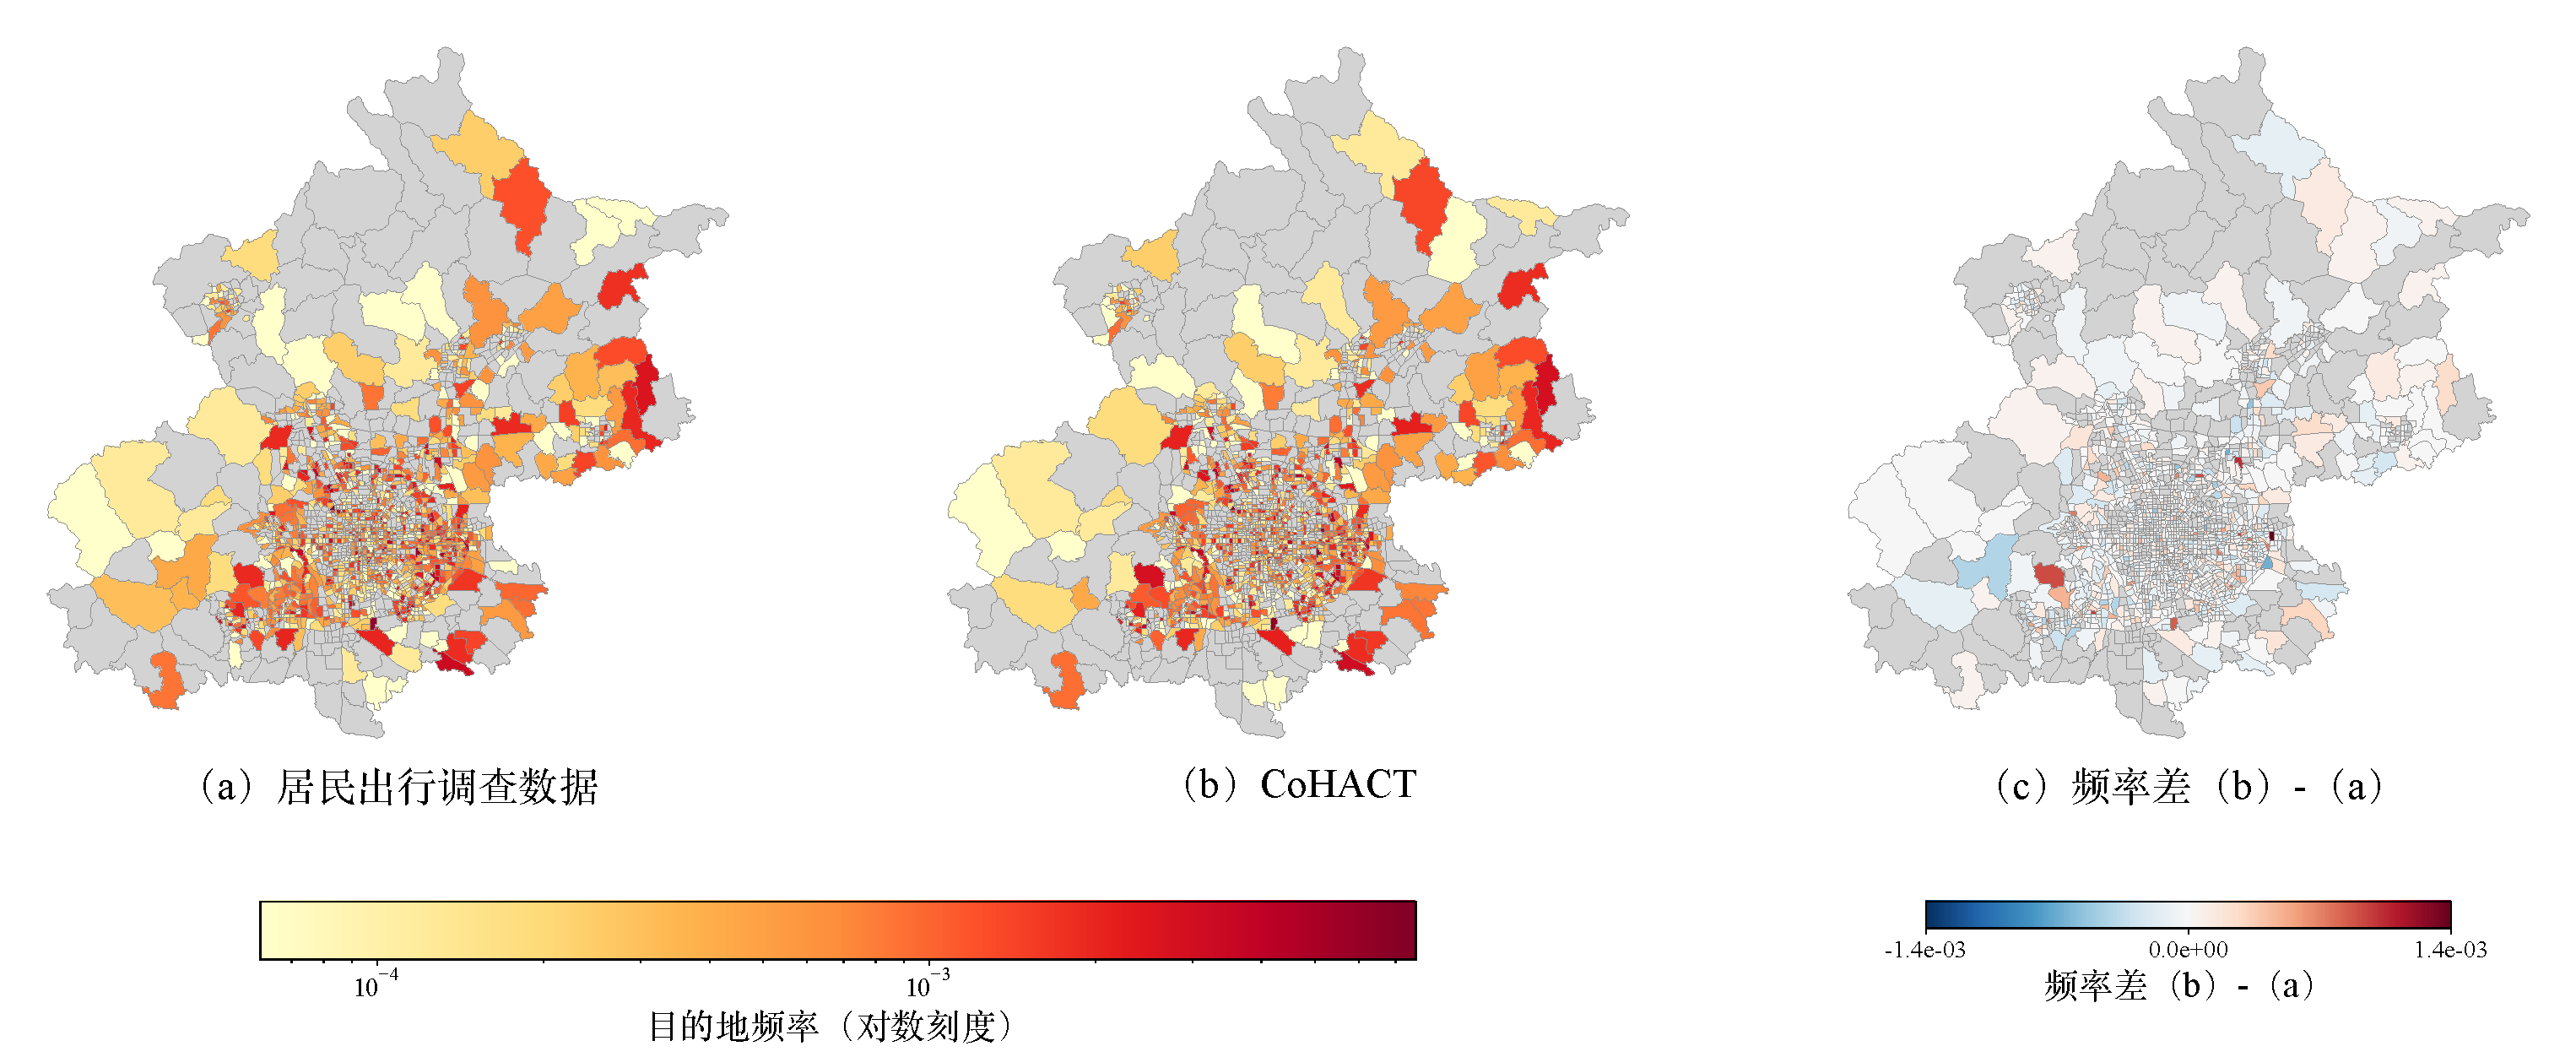
\includegraphics[width=\textwidth]{figures/ch4/destination_choropleth_cn.pdf}
  \bicaption{目的地空间分布对比}{Comparison of destination spatial distributions.}
  \label{fig.cohact.choropleth}
\end{figure}
并从两个互补的角度加以评估：一是整体空间格局是否吻合，借助图~\ref{fig.cohact.choropleth} 的空间分布与两分布间的 Jensen-Shannon（JS）散度度量；二是区域覆盖是否完整，借助图~\ref{fig.cohact.coverage} 的长尾覆盖加以检验。

图~\ref{fig.cohact.choropleth} 表明，在总体空间格局方面，CoHACT生成的目的地分布在全市尺度上与真实数据的目的地分布高度相似，二者均反映了城市中心处的高密度核心与外围的热点分布，且二者的频率之差几乎为零。计算两分布间的Jensen-Shannon（JS）散度结果表明，两分布见的JS散度仅为0.0132，极接近于零，说明生成的目的地分布与真实的目的地分布在全市尺度上几乎相同。这一高空间保真度得益于本文提出的考虑空间异质性的目的地注意力层，该层将可学习的目的地嵌入、用地主题与目的吸引力（式\refeq{eq.cohact.zonekey}）同地理阻抗惩罚（式\refeq{eq.cohact.destlogit}）相结合，使模型在为各候选小区评分时既考虑其对特定活动目的的吸引力、又顾及由出发地到该小区的出行阻抗，从而在城市尺度的大候选集上准确还原目的地需求的空间分布。

然而，生成样本中仍存在少量缺失小区。如图~\ref{fig.cohact.coverage} 所示，生成样本再现了真实数据中被访问的 1370 个目的地小区中的 1230 个，覆盖率为 89.8\%；而 140 个未被覆盖的小区均为真实数据中至多被访问十次的小区，合计仅占真实出行总量的极小部分。换句话说，被访问次数较多的目的地小区均被生成样本覆盖，模型仅在访问极其稀疏的长尾小区上存在遗漏。这一现象与前文类别属性中稀有类别被低估的机理一致。在以 Softmax 对全候选集评分的目的地预测中，访问次数极少的小区难以积累足够的训练信号，加之地理阻抗与吸引力机制本就倾向于将选择概率集中于地理邻近且具吸引力的小区。考虑到被遗漏的小区被访问次数极少，其缺失对全市目的地分布的整体保真度影响较小。

\begin{figure}[H]
  \centering
  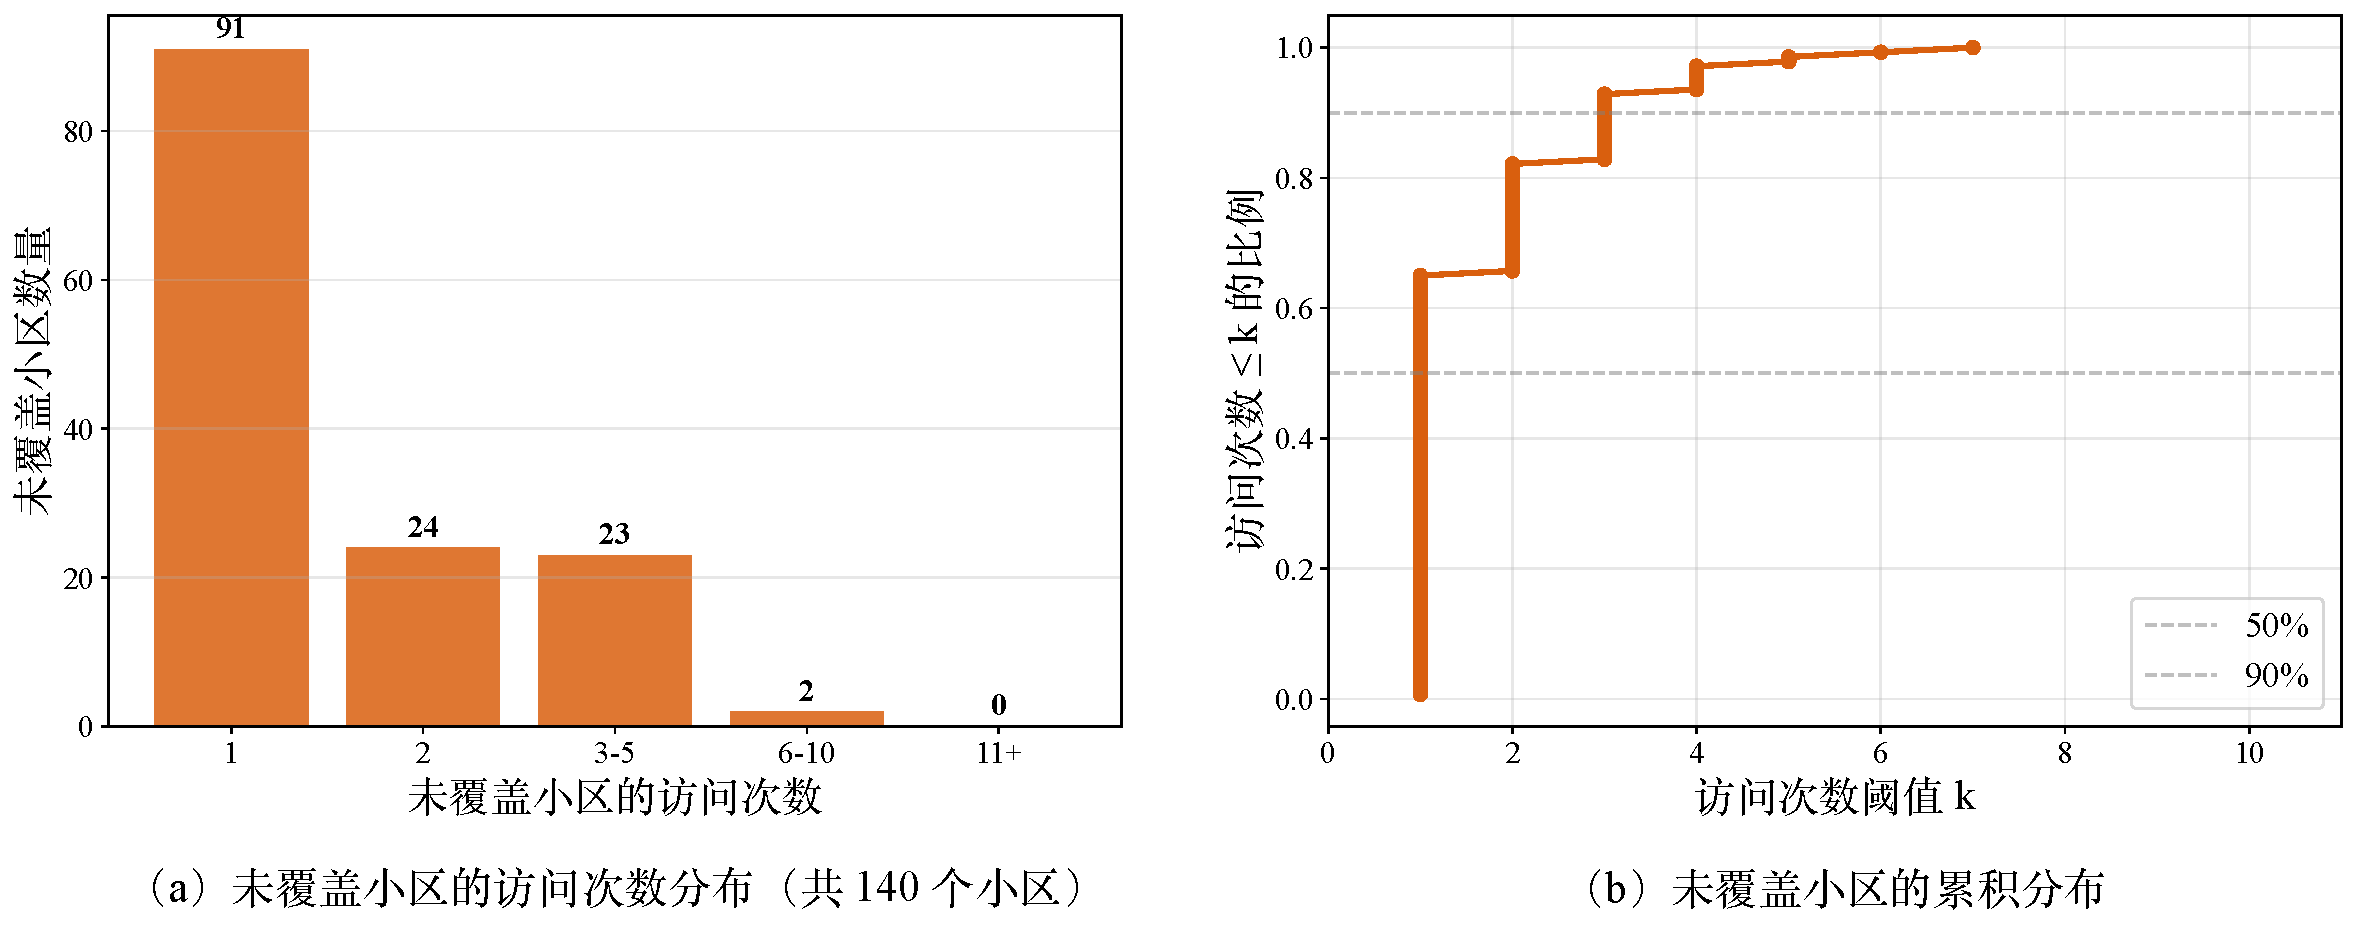
\includegraphics[width=\textwidth]{figures/ch4/coverage_longtail_cn.pdf}
  \bicaption{目的地区域覆盖的长尾验证}{Long-tail validation of destination-zone coverage.}
  \label{fig.cohact.coverage}
\end{figure}

综上，针对目的地空间分布的分析表明，CoHACT 能够在城市尺度的大候选集上高保真地再现真实的目的地选择结果，仅在极少数被访问次数较低的小区上存在遗漏，验证了本章提出的考虑空间异质性的目的地注意力层在城市级目的地选择上的有效性。

%==================================================================
\section{大规模算例实验}\label{sec.cohact.cityexp}

\ref{sec.cohact.experiment}节的小规模算例实验已在测试集上验证了CoHACT的生成精度、家庭协调性与目的地空间保真度。虽然各项实验表明CoHACT在个体级与家庭级均能生成较为真实的活动计划，但其验证尺度（3219户测试家庭）过小，难以为MaaS推广策略仿真优化提供覆盖全市人口的微观行为基础。因此，本节与第\ref{chap.popsyn}章合成的城市级别虚拟人口相衔接，进一步开展大规模算例实验。通过该实验可检验CoHACT在城市尺度下的计算可扩展性、个体级属性分布的真实性以及目的地空间分布的合理性，从而为MaaS推广策略仿真优化提供可靠的微观行为基础。

考虑到CoHACT模型的效果已通过测试集进行了全面的检验，本节仅将其应用于第\ref{chap.popsyn}章合成的全市家庭级虚拟人口，随后依次从生成规模与计算效率（\ref{subsec.cohact.cityexp.scale}小节）、个体级活动计划合理性（\ref{subsec.cohact.cityexp.dist}小节）与目的地空间分布合理性（\ref{subsec.cohact.cityexp.spatial}小节）三个方面展开验证。

\subsection{算例设置}\label{subsec.cohact.cityexp.setup}

\textbf{（1）虚拟人口输入}

大规模算例的生成对象为第\ref{chap.popsyn}章HiDiT模型合成的家庭级虚拟人口，覆盖北京市16个辖区、约1400万户家庭共31582283名虚拟居民，其家庭级与个人级社会经济属性的类别均与本章训练数据相同。与小规模算例的3219户测试家庭相比，本算例的生成对象在规模上扩大了三个数量级以上，且虚拟人口不携带任何真实的活动-出行记录，因而对CoHACT的工程可扩展性与泛化能力构成双重检验。

\textbf{（2）工作地与上学地指派}

CoHACT的生成过程除家庭与成员的社会经济属性外，还须以每位成员的居住小区及其工作地或上学地锚点小区作为空间条件输入；而第\ref{chap.popsyn}章的虚拟人口仅具有1\,km栅格粒度的居住位置，且不含就业地与就学地信息。其中，居住地小区可通过栅格质心和交通小区的空间包含关系直接指派，但工作地与上学地的锚点小区则需通过目的地选择模型进行推断。基于2023年北京市居民出行调查，分别为就业者与学生标定工作地选择与上学地选择两个多项Logit目的地选择模型，再据两模型输出的选择概率为每位虚拟就业者与虚拟学生抽样锚点所在的交通小区。

两模型的备选集均为全市2006个交通小区，效用函数由四类核心变量构成，即居住小区与备选小区间的质心直线距离、备选小区的就业/上学吸引度（基于特征价格模型与地理加权回归度量的就业与学校设施价值）、小区规模与本区虚拟变量，并将收入、车辆拥有情况、年龄、学历与教育阶段等属性同小区间距离及就业/上学吸引度作交互，以刻画目的地选择的群体异质性。模型以居民出行调查中有效的45047名就业者与6546名学生为样本标定，其效用函数设定、估计方法、估计结果与就业/上学吸引度变量的构建流程详见附录~C。

从标定与验证结果看，两模型核心系数的符号均与出行行为直觉一致（距离项显著为负，就业/就学吸引度、小区规模与在本区就业/就学哑元变量显著为正），交互项亦揭示出收入越高的就业者对长距离通勤容忍度越强、学段越高通学范围越大等合理的群体异质性。测试集验证结果表明，模型预测的期望通勤/通学距离与实测均值基本一致（预测期望通勤距离5.63\,km对实际平均通勤距离5.57\,km，预测期望通学距离4.65\,km对实际平均通学距离4.38\,km），具备为虚拟人口指派工作地/就学地的精度基础。据此将两模型应用于全体虚拟人口（其中就业者2458.3万人、学生105.6万人）。

\textbf{（3）验证方式}

与小规模算例不同，第\ref{chap.popsyn}章生成的虚拟居民不存在真实的活动计划，故无法采用将生成的活动计划与真实活动计划对比的方式进行验证。因此，本节转而在分布层面将全市生成结果与居民出行调查数据的全体活动计划进行比较。

\subsection{生成规模与计算效率}\label{subsec.cohact.cityexp.scale}

首先对生成城市级活动计划的可行性进行分析。表~\ref{tab.cohact.cityexp.scale}汇总了北京市16个行政区的活动计划生成规模与耗时。CoHACT共为31582283名虚拟居民生成65190504次出行，人均出行2.064次，较训练数据的2.133次仅低约3.2\%；分区来看，各辖区人均出行介于2.028\,\textasciitilde\,2.099次之间，未随辖区人口规模出现系统性漂移。计算效率方面，在单机单卡环境下生成全市虚拟人口的活动计划累计耗时37.3小时，平均每小时产出约85万名居民的完整活动计划。上述结果表明，CoHACT的生成流程具备扩展至城市级人口的可行性。

{
\small
\begin{longtable}{@{}L{2.0cm}*{4}{C{2.6cm}}@{}}
\bicaption{大规模算例的分区生成规模与耗时}{Generation scale and runtime by district in the large-scale case study.}\label{tab.cohact.cityexp.scale} \\
\toprule
行政区 & 虚拟人口（人） & 出行数（次） & 人均出行（次） & 耗时（小时） \\
\midrule
\endfirsthead
\multicolumn{5}{l}{\small（续表~\ref{tab.cohact.cityexp.scale}）}\\
\toprule
行政区 & 虚拟人口（人） & 出行数（次） & 人均出行（次） & 耗时（小时） \\
\midrule
\endhead
\midrule
\multicolumn{5}{r}{\small 续下页}\\
\endfoot
\bottomrule
\endlastfoot

朝阳区 & 5623754 & 11712852 & 2.083 & 5.2 \\
海淀区 & 5333017 & 10972250 & 2.057  & 4.8 \\
丰台区 & 3632221 & 7498486 & 2.064  & 7.3 \\
昌平区 & 2709519 & 5573239 & 2.057  & 2.5 \\
西城区 & 2302741 & 4762294 & 2.068 & 2.1 \\
大兴区 & 2085396 & 4377605 & 2.099 & 3.8 \\
通州区 & 1684398 & 3435647 & 2.040 & 1.8 \\
东城区 & 1650724 & 3348462 & 2.028 & 3.2 \\
顺义区 & 1493523 & 3059621 & 2.049 & 1.5 \\
房山区 & 1400939 & 2916978 & 2.082 & 1.5 \\
石景山区 & 1079065 & 2189187 & 2.029 & 0.9 \\
密云区 & 666405 & 1372204 & 2.059 & 0.7 \\
平谷区 & 617825 & 1260286 & 2.040 & 0.6 \\
怀柔区 & 515737 & 1081304 & 2.097 & 0.6 \\
延庆区 & 419452 & 872465 & 2.080 & 0.5 \\
门头沟区 & 367567 & 757624 & 2.061 & 0.4 \\
\midrule
合计 & 31582283 & 65190504 & 2.064 & 37.3 \\
\end{longtable}
}

\subsection{个体级活动计划属性分布}\label{subsec.cohact.cityexp.dist}

考虑到\ref{sec.cohact.experiment}节已对CoHACT模型展开了较为全面的验证，本节仅在分布层面对大规模生成的活动计划进行验证。沿用\ref{subsec.cohact.experiment.dist}小节的验证方式，将大规模生成的活动计划与居民出行调查数据在六个属性（出发地与目的地除外）的一维边际分布上逐一比较（图~\ref{fig.cohact.cityexp.marginals}）。须说明的是，因对比两侧的样本量相差悬殊（生成侧65190504次出行、居民出行调查侧147322条出行），各图纵轴以设定为对数坐标下的频率。

\begin{figure}[H]
  \centering
  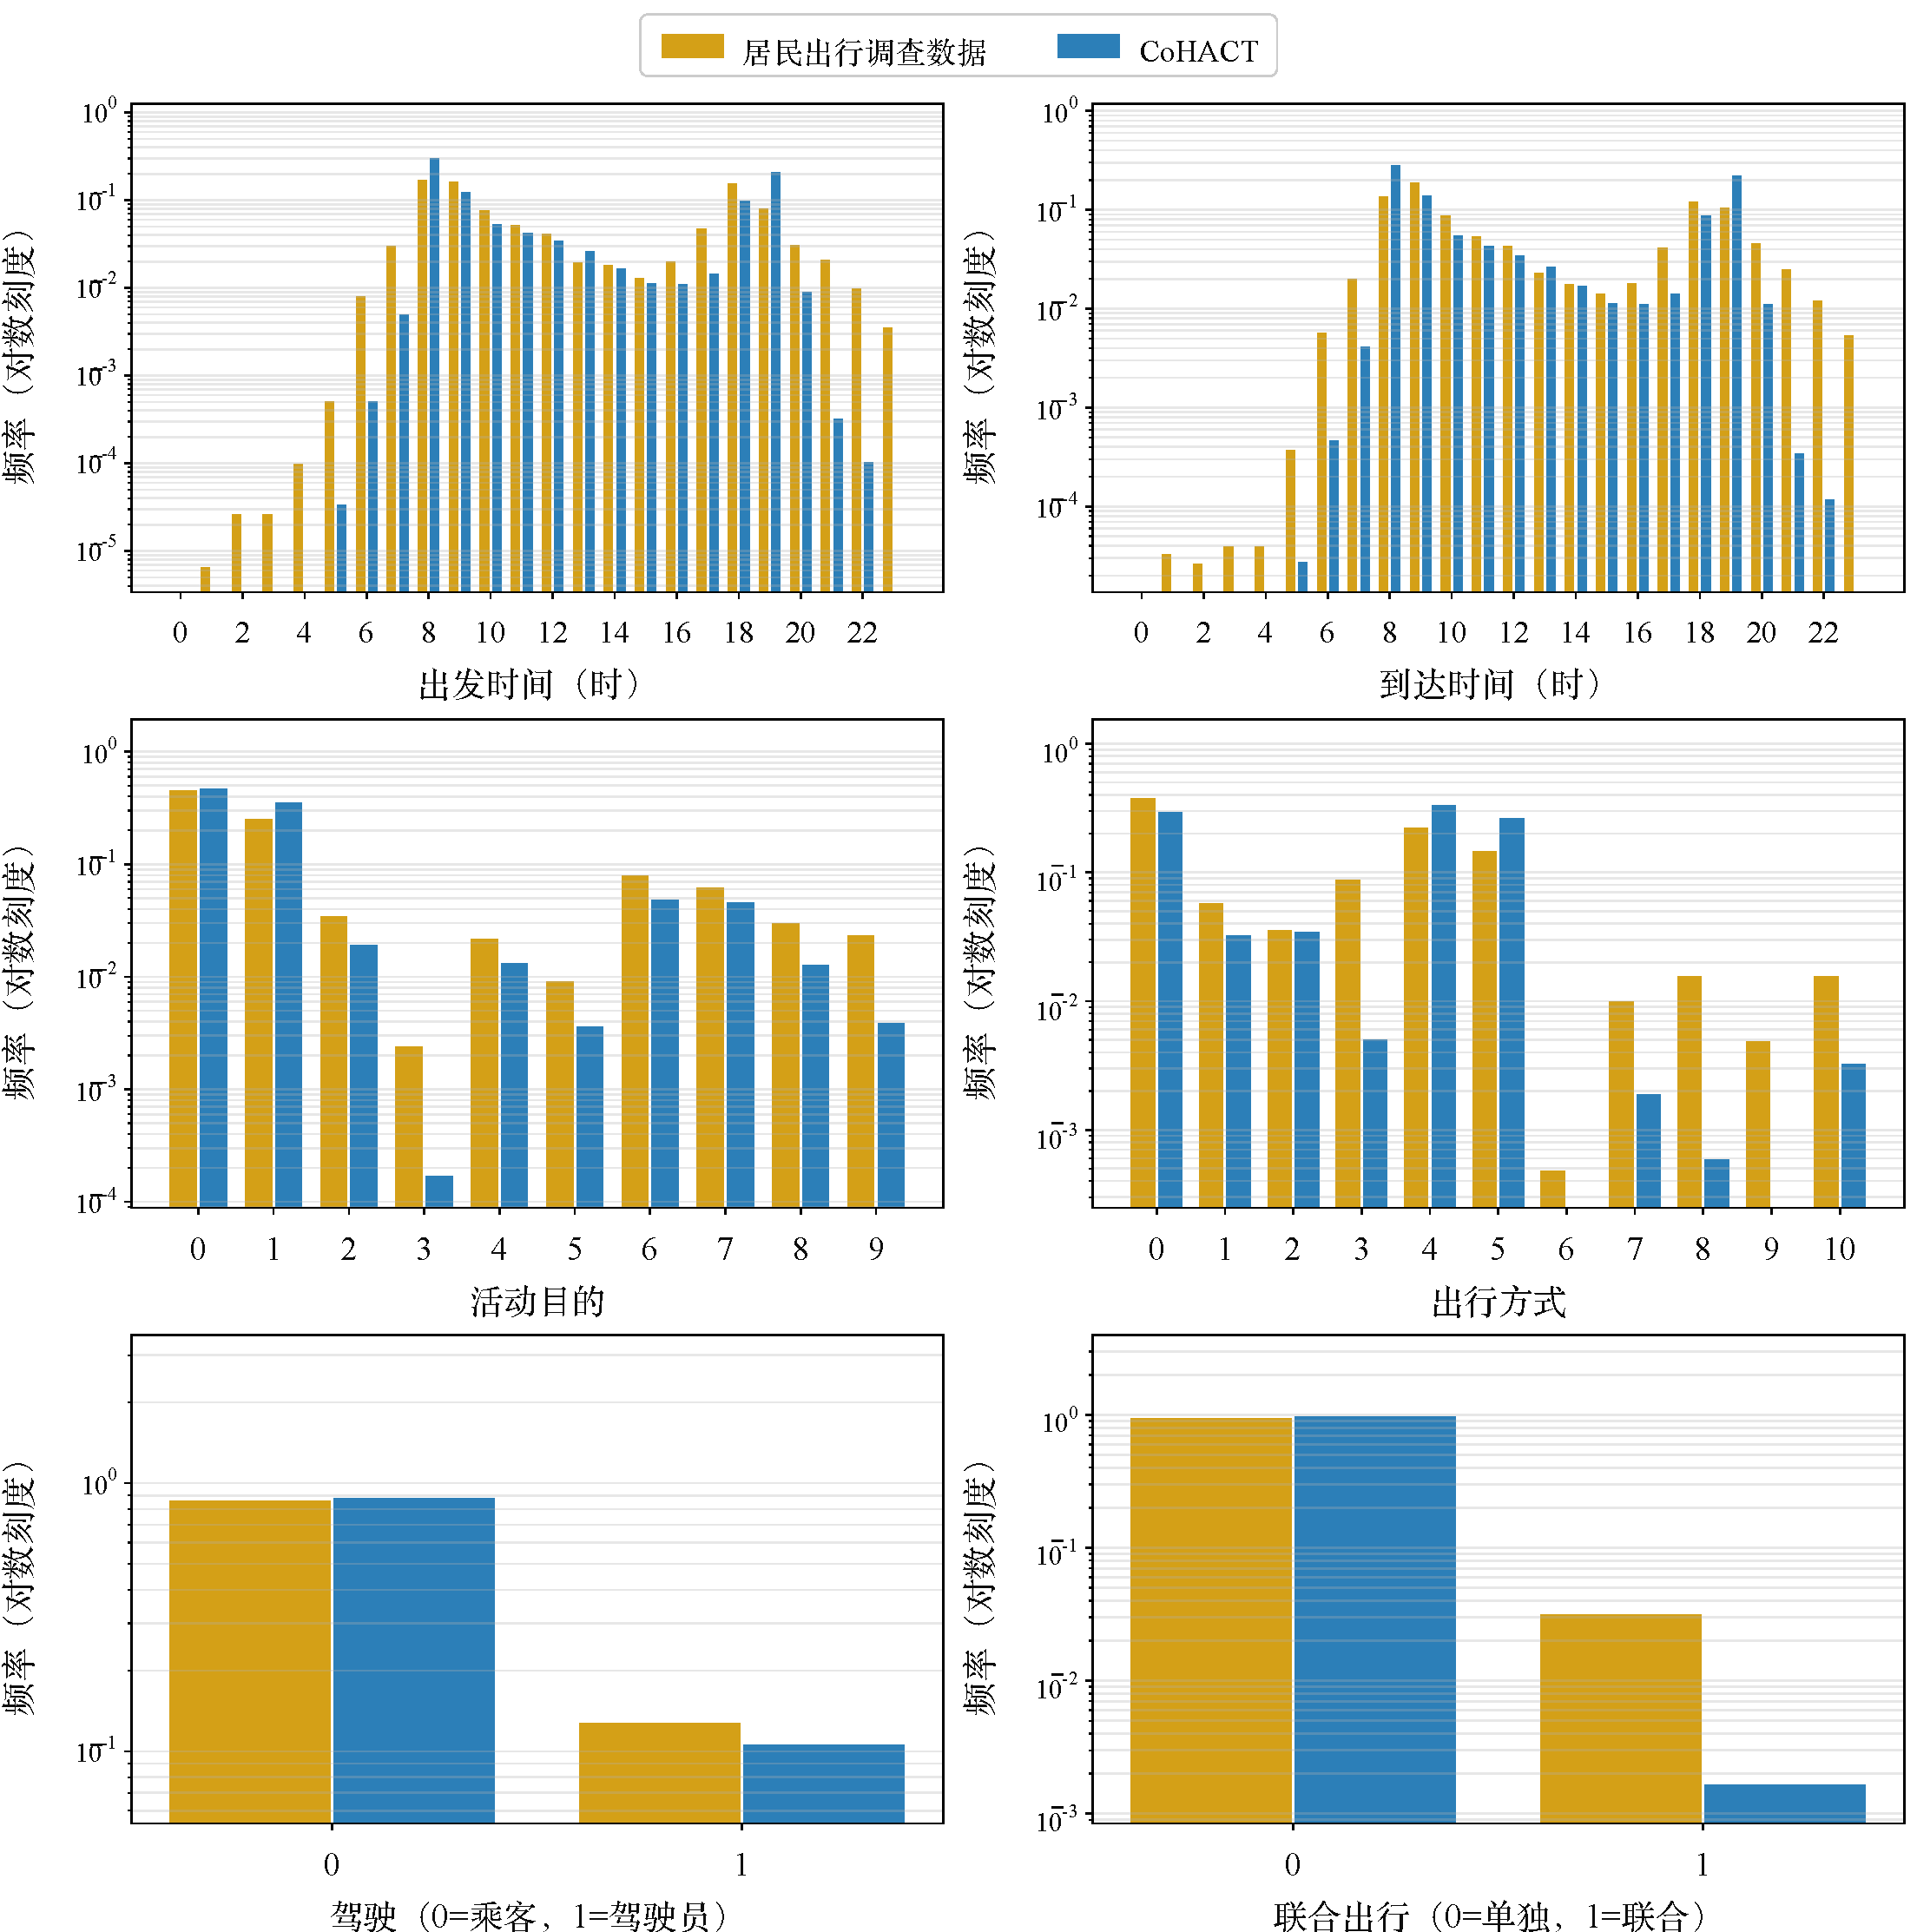
\includegraphics[width=\textwidth]{figures/ch4/city_marginals_6attr_cn.pdf}
  \bicaption{大规模生成活动计划与居民出行调查数据的一维边际分布对比}{Comparison of one-dimensional marginal distributions between activity generated in the large-scale case study and household travel survey data.}
  \label{fig.cohact.cityexp.marginals}
\end{figure}

图~\ref{fig.cohact.cityexp.marginals}表明，大规模生成的活动计划在六个属性的边际分布上均保持了与居民出行调查中的活动计划较为一致的整体形态。在时间属性上，出发时间与到达时间子图显示CoHACT在全市尺度上较为完整地复现了居民一日出行的双峰节律：两侧早高峰均位于8时、晚高峰均位于18\,\textasciitilde\,19时。在活动目的与出行方式两个类别属性上，主导类别及其排序均与居民出行调查一致：回家与工作居活动目的的前两位，步行、电动自行车与小汽车为份额最高的三种出行方式，地铁份额与居民出行调查数据几乎持平。偏差的方向则与小规模算例中已识别的生成精度特征一致，即高估电动自行车与小汽车所占份额，低估步行、自行车与公交的所占份额。在两个家庭协调相关属性上，驾驶标识的边际分布与参照接近；联合出行标识则被部分低估。

以上对比结果表明，在城市级居民活动计划任务中，CoHACT在个体级活动计划属性分布上仍保持了与居民出行调查数据的整体一致性，且偏差的方向与小规模算例中量化的生成精度特征一致。换言之，CoHACT无需任何重新训练，即可在城市级人口上保持其在小规模算例中已验证的生成精度特征。

\subsection{目的地空间分布}\label{subsec.cohact.cityexp.spatial}

上一节针对CoHACT模型在个体级活动计划属性分布上的真实性进行了验证，本节进一步考察大规模生成的活动计划在目的地空间分布上的合理性。沿用\ref{subsec.cohact.experiment.spatial}小节的验证方式，在全市2006个交通小区上将大规模生成样本的目的地分布与居民出行调查的目的地分布进行比较：绘制两者的空间分布并计算频率之差（图~\ref{fig.cohact.cityexp.choropleth}），进而计算两分布间的JS散度与热点小区重叠情况。

\begin{figure}[H]
  \centering
  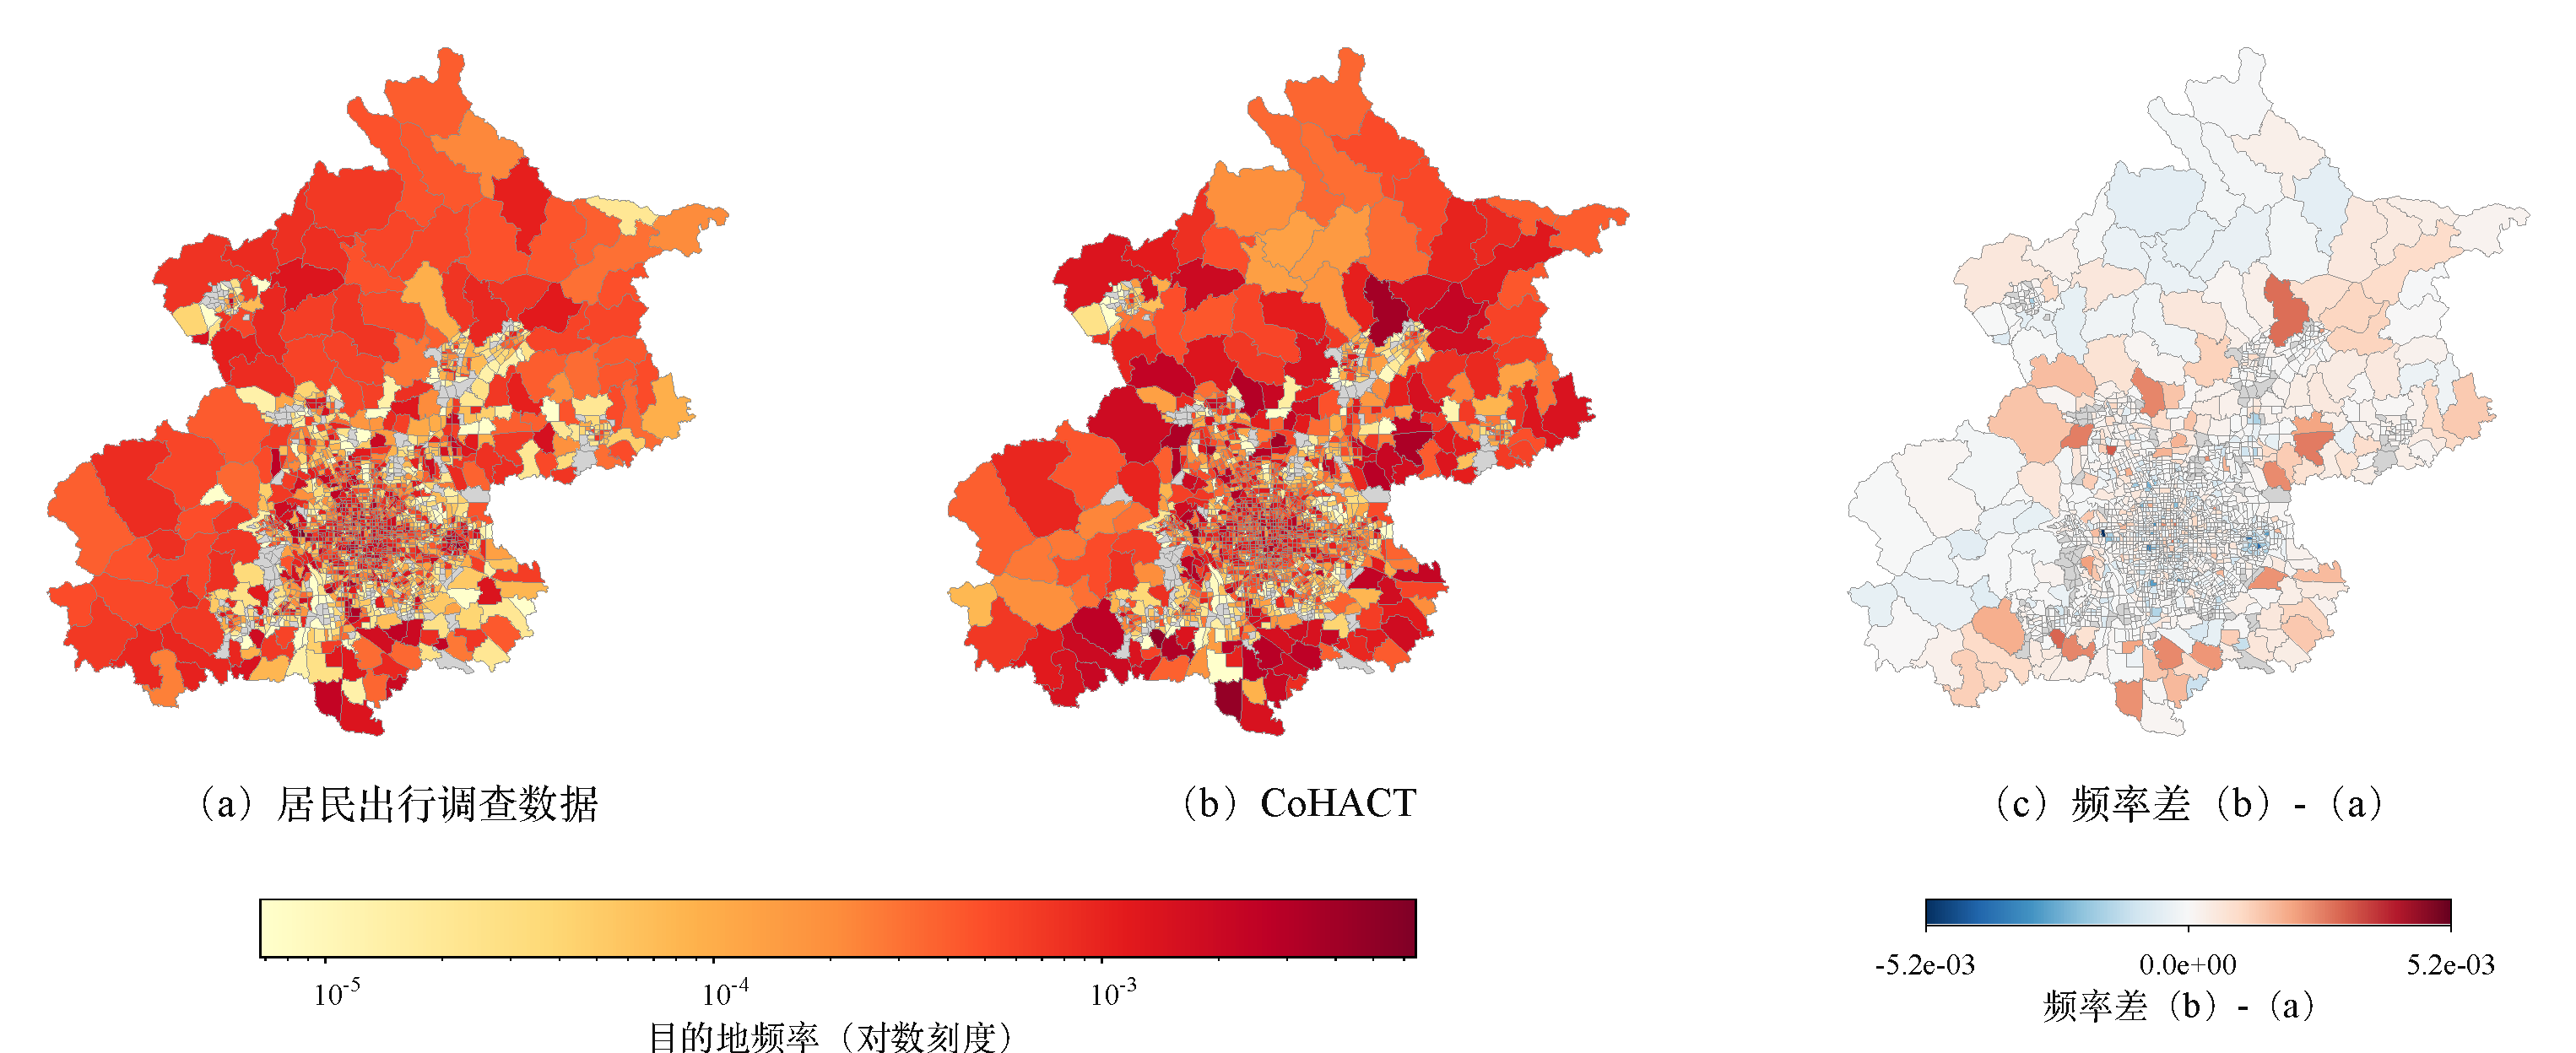
\includegraphics[width=\textwidth]{figures/ch4/city_destination_choropleth_cn.pdf}
  \bicaption{目的地空间分布对比}{Comparison of destination spatial distributions.}
  \label{fig.cohact.cityexp.choropleth}
\end{figure}

图~\ref{fig.cohact.cityexp.choropleth}表明，在总体空间格局上，大规模生成的目的地分布与居民出行调查高度相似，即二者的目的地分布均集中于中心城区与外围部分交通小区，二者的空间分布在对数尺度下也呈现出一致空间分布模式（JS散度为0.0730）。具体而言，绝大多数小区目的地分布的频率之差接近零（差值绝对值不超过$5.2\times10^{-3}$）。CoHACT生成的样本共覆盖1808个目的地小区（占全部2006个小区的90.1\%），与居民出行调查包含的1808个小区几乎重合（共同的交通小区有1802个），未被覆盖的小区仍集中于访问极稀疏的长尾低吸引小区。

综上，CoHACT在城市级人口上生成的活动计划在目的地空间分布上仍保持了与居民出行调查数据的整体一致性。

%==================================================================
\section{本章小结}\label{sec.cohact.summary}

本章针对MaaS推广策略仿真所需的高保真活动计划输入，研究了考虑家庭联合活动的家庭级活动计划生成问题。既有研究多以个体为基本生成单元，将居民视作彼此独立的样本，难以再现联合出行、车辆共享与接送等家庭联合活动行为，致使生成的活动计划在联合出行、接送与车辆分配等家庭级统计上产生偏差。围绕家庭与成员多层级信息的统一感知、多成员活动计划的协调生成以及城市级目的地选择的建模三方面困难，本章以第\ref{chap.popsyn}章合成的家庭级虚拟人口为输入，提出了协调式家庭活动计划生成框架（CoHACT），并以北京市为算例，依次开展了基于居民出行调查数据的小规模算例实验与面向全市虚拟人口的大规模算例实验。本章的主要工作与结论如下。

其一，针对家庭与成员多层级信息的统一感知，构建了融合家庭-成员特征的多任务编码器。该编码器以渐进分层提取结构为主体，将家庭表征与成员表征的提取建模为多任务学习问题，通过定制化门控机制显式分离共享专家与任务专属专家，缓解两类特征间的负迁移；其专家以诱导集合注意力块实现，使家庭成员表征对家庭内成员的次序保持置换等变、适应可变的家庭规模，并在聚合中令各成员蕴含家庭层面的共享信息。在此基础上，进一步由独立训练并冻结权重的活动模式识别模型构建家庭级与个人级活动模式先验，缓解由属性到活动链的``一对多''映射、压缩生成空间。

其二，针对家庭内多成员活动计划的协调生成，设计了考虑家庭联合活动的多任务学习解码器。该解码器先经任务特定注意力与跨角色注意力使各成员在生成前相互感知、形成蕴含家庭情境的协调成员特征，再以多任务注意力网络逐属性、自回归地同时生成全体成员的活动计划，并经自适应层归一化将活动模式先验注入生成过程。算例表明，CoHACT在个体与家庭两个层面、全部属性组合维度下均显著优于GAN、VAE及其条件版本等六个基准模型：最严格的8维联合分布下SRMSE低至1.95，约为最优基准（CGAN，30.06）的1/15；且生成误差几乎不随属性维度恶化（由4维的1.69仅微增至8维的1.95），表明逐属性、自回归的联合建模有效保持了高维属性间的依赖。

其三，针对家庭内部车辆共享、联合出行与接送等耦合关系硬约束的限制，提出了基于纳什议价的家庭活动计划协调层。该层将家庭活动计划协调建模为纳什议价问题，以解码器输出为分歧点，求解一个帕累托有效、个体理性且在成员间均衡分配效用增益的可行解，并经``序列二次规划求可行解、可微二次规划回传梯度''的两阶段算法实现与编码器、解码器的端到端联合训练，在严格满足车辆可用性等硬约束的同时最大化家庭整体效用。消融实验表明，移除该层后家庭层面的Household-SRMSE由1.48升至2.18、6维子集的SRMSE由4.31升至5.62；家庭级协调性分析进一步表明，CoHACT生成的全部3219户家庭活动计划均不存在车辆超配，与真实调查完全一致，而移除该层后车辆超配家庭占比升至17.3\%，凸显了该层在保证家庭级可行性上的关键作用。

其四，针对城市级目的地选择的建模，设计了考虑空间异质性的目的地注意力层。该层以可学习的目的地嵌入、用地主题向量与目的吸引力向量异质地表征候选小区，并在注意力评分中融入地理阻抗惩罚与目的吸引力加成，在数千个候选交通小区构成的大候选集上刻画情境依赖、空间异质的目的地选择，同时以距离感知的出行方式预测头耦合目的地与出行方式预测。算例表明，CoHACT生成的目的地分布与真实分布的JS散度仅为0.0132、二者在全市尺度上几乎一致，并完整覆盖了被访问次数较多的交通小区（覆盖率89.8\%，仅遗漏了至多被访问十次的长尾低访问需求小区）；消融实验中移除该层将导致所有含出发地与目的地预测的子集精度显著变差，从正反两方面验证了该层在城市级目的地选择上的有效性。

其五，为检验方法在城市级应用中的可扩展性与泛化能力，开展了面向全市虚拟人口的大规模算例实验。经居住小区匹配与基于新标定目的地选择模型的工作地/就学地指派等前期数据处理工作，将训练完成的CoHACT不经任何重新训练直接应用于第\ref{chap.popsyn}章合成的约1400万户虚拟家庭，在单机环境下以37.3小时为31582283名虚拟居民生成了由65190504次出行构成的活动计划，人均出行次数（2.064次）与居民出行调查基本一致。分布层面的对比验证表明，生成结果在时间节律、类别构成、目的地空间分布上均保持了与真实出行行为一致的总体结构，偏差方向与机理均与小规模算例一致。

综上，本章提出的CoHACT框架能够在严格满足家庭资源约束与联合活动约束的前提下，生成个体属性真实、家庭内部活动协调且目的地空间精度高的家庭级活动计划。所生成的活动计划完整刻画了每位居民一日之内的活动-出行序列及其家庭协调关系。大规模算例产出的覆盖全市的活动计划可直接作为第\ref{chap.optimization}章推广策略仿真优化中智能体现有的出行模式，为MaaS推广策略仿真界定了各智能体向MaaS转移的具体情境，与\ref{chap.popsyn}章合成的虚拟人口共同构成了仿真的微观行为基础。
